\documentclass[
  normalmargins,
  10pt,
  openany,
  onehalfspacing,
]{my-format}
% packages
\usepackage[colorlinks]{hyperref} % for links
\usepackage[dvipsnames]{xcolor}
\usepackage{acro}
\usepackage{fancyhdr} 
\pagestyle{fancy}

\DeclareAcronym{CC}{
  short=CC,
  long=Cross-Correlation,
    }
\DeclareAcronym{CP-OTDR}{
  short=CP-OTDR,
  long=Chirped Pulse OTDR,
    }
\DeclareAcronym{DFB}{
  short=DFB,
  long=Distributed Feedback,
    }
\DeclareAcronym{EDFA}{
  short=EDFA,
  long=Erbium Doped Fiber Amplifier,
    }
\DeclareAcronym{FBG}{
  short=FBG ,
  long=Fiber Bragg Grating,
    }
\DeclareAcronym{FFT}{
  short=FFT,
  long=Fast Fourier Transform,
    }
\DeclareAcronym{FP}{
  short=FP,
  long=Fabry-Pérot,
    }
\DeclareAcronym{FUT}{
  short=FUT,
  long=Fiber Under Test,
    }
\DeclareAcronym{FWHM}{
  short=FWHM,
  long=Full Width at Half Maximum,
    }
\DeclareAcronym{MWE}{
  short=MWE,
  long=Maxwell's Equations,
    }
\DeclareAcronym{NIR}{
  short=NIR,
  long=Near-Infrared,
    }
\DeclareAcronym{NLSE}{
  short=NLSE,
  long=Nonlinear Schrodinger equation,
    }
\DeclareAcronym{OFDR}{
  short=OFDR,
  long=Optical Frequency Domain Reflectometry,
    }
\DeclareAcronym{OPD}{
  short=OPD,
  long=Optical Path Difference,
    }
\DeclareAcronym{OTDR}{
  short=OTDR,
  long=Optical Time Domain Reflectometry,
    }
\DeclareAcronym{P-OTDR}{
  short=P-OTDR,
  long=Polarization OTDR,
    }
\DeclareAcronym{PIC}{
  short=PIC,
  long=Photonic Integrated Circuit,
    }
\DeclareAcronym{RFGA}{
  short=RFGA,
  long=Random Fiber Grating Array,
    }
\DeclareAcronym{SOA}{
  short=SOA,
  long=Solid State Optical Amplifier,
    }
\DeclareAcronym{SOP}{
  short=SOP,
  long=State of Polarization,
    }
\DeclareAcronym{SOTA}{
  short=SOTA,
  long=State of the Art,
    }
\DeclareAcronym{SSFM}{
  short=SSFM,
  long=Split-Step Fourier Method,
    }
\DeclareAcronym{TDR}{
  short=TDR,
  long=Time Doman Reflectometry,
    }
\DeclareAcronym{UV}{
  short=UV,
  long=Ultraviolet,
    }
\DeclareAcronym{WSS}{
  short=WSS,
  long=Wavelength Selective Switch,
    }
    
    
    
    
\usepackage[many]{tcolorbox}    	% for COLORED BOXES (tikz and xcolor included)
\newtcolorbox{boxA}{
    fontupper = \bf,
    boxrule = 1.5pt,
    colframe = black % frame color
}
\newcommand{\A}{\textcolor{red}{A}} 
\newcommand{\E}{\textcolor{red}{E}} 
\newcommand{\greencheck}{\textcolor{green}{\checkmark}}
\newcommand{\redcross}{\textcolor{red}{x}}


\newcommand{\betag}{\textcolor{ForestGreen}{\beta}} 
\newcommand{\CITE}{\textcolor{magenta}{CITE?!?!?!?!?!}} 
\newcommand{\real}{\mathfrak{Re}}
\newcommand{\FT}{\mathfrak{F}}
\newcommand{\IFT}{\mathfrak{F}^{-1}}



\usepackage{amsmath}
\usepackage{amsfonts}
\usepackage{graphicx} % for embedding graphics
\usepackage{booktabs} % for pretty tables
\usepackage{pgfplots}
\pgfplotsset{compat=1.18,width=11cm}
\usetikzlibrary{math}
\usepackage[all]{nowidow}
\usepackage{pdflscape}
\usepackage[final]{pdfpages}
\usepackage{afterpage}
\usepackage[nottoc]{tocbibind}
\usepackage{amssymb}
\usepackage{changepage}

\newcommand{\degs}{^{\circ}}
\newcommand{\inv}{$^{-1}$}


% author data
\author{Ole Krarup}
\title{\Large A primer on the Nonlinear Schr{\"o}dinger Equation }

% reference database



\begin{document}
 
  \frontmatter    
        
    \maketitle
    \addtocounter{page}{1}
    
   
   
    \addcontentsline{toc}{chapter}{Table of Contents}
    \tableofcontents
    
    \listoffigures
    \listoftables
    
    %
\color{white}
    \begin{tiny}
        \ac{CC}
        \ac{CP-OTDR}
        \ac{DFB}
        \ac{EDFA}
        \ac{FBG}
        \ac{FFT}
        \ac{FP}
        \ac{FUT}
        \ac{FWHM}
        \ac{MWE}
        %\ac{NIR}
        \ac{NLSE}
        \ac{OFDR}
        \ac{OPD}
        \ac{OTDR}
        \ac{P-OTDR}
        %\ac{PIC}
        \ac{RFGA}
        \ac{SOA}
        \ac{SOP}
        \ac{SOTA}
        \ac{SSFM}
        \ac{TDR}
        %\ac{UV}
        %\ac{WSS}
        
    \end{tiny}
\color{black}
    %\printacronyms
    %\addcontentsline{toc}{chapter}{List of Acronyms}
    
    \mainmatter
    
    \pagestyle{plain}
    \chapter{介绍}
\label{ch:Introduction}
广义标量形式的非线性薛定谔方程(NLSE)描述了复电场的归一化包络 \(\A = \A(z,T)\) 如何随传播介质中的传播而演变。在该介质中存在损耗(α)、色散(β)和 \(\chi^{3}\) 非线性(γ)。复电场的形式为 \(\E = \E(z,T) = \E_0 \cdot \exp(-i(\betag(\omega_0)z - \omega_0 T))\),其振荡频率为载波角频率 \(\omega_0\),载波空间频率为 \(\betag(\omega_0)\)。广义非线性薛定谔方程的数学表达式如下:
\begin{align}
    \label{eq:GNLSE}
    \partial_z \A = \frac{\alpha}{2}\A+i \sum_{n=2}^{\infty}i^n \frac{\betag_n}{n!}\partial_T^n\A  + i\gamma\left(1+\frac{i}{\omega_0}\partial_T  \right)\left( 
\A \int_{0}^{\infty} R(T_{delay})|\A(z,T-T_{delay})|^2 dT_{delay} \right),
\end{align}
其中,\(\alpha\) 是功率衰减/增益系数,\(\betag_n = \partial_\omega^n \betag(\omega)|_{\omega = \omega_0}\) 是在 \(\omega = \omega_0\) 处计算的空间频率泰勒展开系数,\(\gamma\) 是非线性系数,\(R(T_{delay})\) 是在当前时刻 \(T\) 之前 \(T_{delay}\) 时间延迟处的非线性时间响应函数。通过求解方程 Eq.~\ref{eq:GNLSE},可以描述超连续谱生成~\cite{supercontinuum_original_paper,NLSE_original}、孤子~\cite{soliton_first_theory,Soliton_experimental_first}、光纤通信系统中的非线性噪声~\cite{poggiolini2014detailedanalyticalderivationgn} 以及其他具有广泛科学和工业应用的奇异光学现象。
\section{目标}
本入门指南旨在以直观的方式探讨方程 Eq.~\ref{eq:GNLSE} 的组成项及其相互作用,旨在帮助读者理解背后的数学和物理基础。为了实现这一目标,本指南舍弃了更复杂的效应讨论,例如涉及光的偏振的影响,而更注重纯粹标量效应的详细推导和示例。希望这种方法能够为读者提供分析非线性光学中常见实验结果的基本工具,同时也为深入研究相关主题的资源、论文和教科书打下基础。

\section{可获取性}
本入门指南可在 \href{https://github.com/OleKrarup123/NLSE-primer}{GitHub} 免费获取,作者会根据读者的反馈不断更新。鼓励读者提交问题、建议和意见至 \href{yourfavouriteta@gmail.com}{YourFavouriteTA@gmail.com}。

\section{引用政策}
本指南引用了所探讨主题的原创学术研究成果,并提供了一些链接,例如 YouTube 视频、个人网页、在线百科全书条目、互动工具等,这些内容由业余爱好者和专业研究人员共同创作。目的在于为读者提供一个全面回顾正式文献的起点,以便他们可以独立撰写关于非线性光学的论文或学位论文,同时也帮助他们深入理解该主题的高质量、易于理解的解释材料。

\subsection{关于引用本入门指南}
本指南并不包含关于 NLSE 的原创研究,应被视为详细笔记的集合。在撰写新的 NLSE 研究论文或学位论文时,不应将本指南作为引用来源。相反,请引用相关主题的最早期的原创文献,例如孤子研究时可引用~\cite{soliton_first_theory} 和~\cite{Soliton_experimental_first}。然而,如果目的是帮助读者熟悉 NLSE 以便更好地理解原创研究,则可以使用以下 BibTeX 格式引用本指南~\cite{NLSE_primer}:

\begin{boxA}
@misc\{NLSE\_primer,  \\  
author = "O. Krarup", \\  
title = "\{A Primer on the Nonlinear Schrödinger Equation\}", \\  
note = "Commit SHA: 9f1b93a", \\  
url = \{https://github.com/OleKrarup123/NLSE-primer/blob/main/NLSE\_primer.pdf\}\}  
\end{boxA}

请注意,由于本指南在 GitHub 上可自由获取且会持续更新,URL 应链接到最新版本,而 "Commit SHA" 应为引用时最新的提交版本号。    
    \chapter{数学和理论}
\label{ch:MathAndTheory}

本章介绍描述电磁波和理解方程~\ref{eq:GNLSE} 所需的基本数学工具。

\section{实数场和复数场}
%Explain that the real field is what determines how an electron moves and that the complex one is only used for mathematical convenience when dealing with phase shifts.
带电荷$q$、质量$m$的粒子在电场 $\Bar{\E}_r = \E_r \hat{x}$ 作用下的加速度为
\begin{align}
    \Bar{a} &=  \frac{q\E_r}{m}\hat{x}.
\end{align}
电场下标$r$表示这是“实”电场,它决定了带电粒子的加速度。而“复”电场则是一种数学工具,使得涉及电磁波的计算更为简便,并且可以始终从中恢复出实电场。例如,传播在体介质中的实电场波,其空间角频率 $\betag$ 依赖于时间角频率 $\omega$,可以表示为:\begin{align}
\label{eq:real_field}
    \E_r(z,t) &= |\E_0|\cos\left(\betag(\omega)z-\omega t+\phi\right) \\\nonumber 
     &=|\E_0| \real\left\{  \exp\left( i\betag(\omega)z-i\omega t+i\phi \right) \right\} \\ \nonumber 
     &= \real\left\{ \E_0 \exp\left( i\betag(\omega)z-i\omega t\right) \right\}  \\ \nonumber
     &= \real\left\{ \E(z,t) \right\}  \\ \nonumber
     &=  \frac{1}{2}\left( \E(z,t) + \E^*(z,t) \right).   
\end{align}
关于方程 \ref{eq:real_field} 的说明,请参见 \href{https://www.desmos.com/calculator/fgvozursrl}{此交互式图表}。
使用复电场在模拟相位变化和干涉效应时非常方便。例如,要在实际电场中引入相位移 $\phi_0$,必须通过以下方式“手动插入”:\begin{align}
\label{eq:insert_phase}
    \E_r(z,t) &= |\E_0|\cos\left(\betag(\omega)z-\omega t+\phi\right) \Rightarrow \\ \nonumber \E_r'(z,t) &= |\E_0|\cos\left(\betag(\omega)z-\omega t+\phi+\phi_0^{\textcolor{Red}{\swarrow}}\right).   
\end{align}
使用复电场,相同的操作可以通过复数乘法来完成,因为
\begin{align}
\label{eq:insert_phase_complex}
    \E(z,t) &=\E_0 \exp\left( i\betag(\omega)z-i\omega t+ i\phi\right)\Rightarrow \\ \nonumber \E'(z,t) &=  \E_0 \exp\left( i\betag(\omega)z-i\omega t +i\phi\right)\exp\left( i\phi_0\right) \\ \nonumber
    &=\E_0 \exp\left( i\betag(\omega)z-i\omega t +i\phi+ i\phi_0\right) \\ \nonumber
    \E_r'(z,t) &= \real\left\{  \E'(z,t)   \right\}. 
\end{align}

此外,由于振荡的实电场的瞬时功率与其平方成正比,平均功率可以通过积分计算或通过复电场绝对值平方的一半来计算,
\begin{align}
\label{eq:average_power}
    \langle \E_r^2 \rangle_T&= \frac{1}{T}\int_{0}^{T} \E_r^2 dt = \langle\real\left\{\E\right\}^2\rangle_T =\frac{1}{4}\langle\left(\E+\E^*\right)^2\rangle_T\\ \nonumber
&=\frac{1}{4}\langle \E^2+\E^{*2}+2|\E|^2 \rangle_T=\frac{1}{2} \langle|\E|^2\rangle_T=\frac{1}{2}|\E|^2.
\end{align}
使用复电场替代“手动插入”和积分的便利性足以使得采用复电场进行计算并仅在必要时提取实电场变得值得。因此,本简介主要利用复电场,但强调这些仅是有用的数学抽象,而实电场具有物理意义,因为它们直接决定了电荷的加速。
\subsection{实际电场和电场包络}
无线电信号用于Wi-Fi的载波频率约为5 GHz,而最先进的示波器可以测量频率高达100 GHz的电场。相比之下,激光脉冲的电场通常在100 THz以上的载波频率下振荡。因此,以实际复电场 \(\E(z,t) = \E_0 \exp\left( i\betag(\omega_0)z - i\omega_0 t\right)\) 进行计算和表达结果往往不够方便,因为以 \(\omega_0/2\pi\) 次每秒发生的快速电场振荡实际上是无法检测到的。相反,我们可以将复电场的包络定义为
\begin{align}
\label{eq:envelope}
    \A(z,t) &=a\cdot\E(z,t)\cdot e^{-i(\betag(\omega_0)z-\omega_0t)},
\end{align}
并用它进行计算。在这里,\( a = \sqrt{0.5 \epsilon_0 n c A_{eff}} \),其中 \(\epsilon_0\) 是真空的介电常数,\( n \) 是介质的折射率,\( c \) 是光速,\( A_{eff} \) 是光场横截面的有效面积,是一个归一化常数。将 \(\E\) 按 \( a \) 缩放确保 \(\A\) 具有 \(\sqrt{W}\) 的单位,因此 \( |\A|^2 \) 具有 \( W \) 的单位。通过“提取”快速且不可检测但又是\emph{可预测的}时间和空间振荡,确定电场由于线性和非线性效应而\emph{变化}的方式变得更加简单。有关 \(\E\) 和 \(\A\) 之间差异的示例,请参见此 \href{https://www.desmos.com/calculator/rsw2fn5af6}{交互式图表}。


\section{傅立叶变换}
%Define the Fourier Transform so going from time to frequency and back is well-behaved. 

在本教程中,傅里叶变换及其逆变换被定义为:
\begin{align}
    \Tilde{\E}(z,\omega) &= \FT\left\{\E(z,t)\right\} = \int_{-\infty}^{\infty} \E(z,t) e^{i\omega t} dt, \\ \nonumber
    \E(z,t) &= \IFT\left\{\Tilde{\E}(z,\omega)\right\} = \frac{1}{2\pi} \int_{-\infty}^{\infty} \Tilde{\E}(z,\omega) e^{-i\omega t} d\omega.
\end{align}
使用 $\exp(i\omega t)$ 的傅里叶变换约定,而不是 $\exp(-i\omega t)$,是因为沿着正 z 方向传播的复平面波由 $\exp(i\betag(\omega_0)z-i\omega_0 t)$ 描述。因此,计算,

\begin{align}
    \FT\left\{\exp(i\betag(\omega_0)z-i\omega_0 t)\right\} &= \int_{-\infty}^{\infty} e^{i\betag(\omega_0)z-i\omega_0 t} e^{i\omega t} dt, \\ \nonumber
      &= \int_{-\infty}^{\infty} e^{i\betag(\omega_0)z-i(\omega_0-\omega) t} dt \\ \nonumber
      &= e^{i\betag(\omega_0)z}\delta(\omega-\omega_0),
\end{align} 
显示复平面波的傅里叶变换产生一个以正载波角频率 $\omega$ 为中心的 δ 函数。如果在傅里叶变换中使用 $\exp(-i\omega t)$ 并将其应用于沿正 z 方向传播的复平面波,结果将包含 $\delta(\omega_0+\omega)$,这意味着 δ 函数是以负载波角频率为中心的。后一种方法使得在涉及沿 z 方向传播的复平面波的傅里叶变换的计算中更复杂,因此采用前一种约定。

\section{脉冲}
在介质中具有有限持续时间的电磁脉冲可以视为一组不同的复平面波的无限和,如下所示:
\begin{align}
    \label{eq:pulse}
    \E(z,t) &= \frac{1}{2\pi}\int_{-\infty}^{\infty} |\Tilde{\E}(z,\omega)| e^{i\betag(z,\omega)z-i\omega t+i\phi(z,\omega)} d\omega \\ \nonumber
    \E(z,t) &= \frac{1}{2\pi}\int_{-\infty}^{\infty} \Tilde{\E}(z,\omega) e^{i\betag(z,\omega)z-i\omega t} d\omega.
\end{align}
方程~\ref{eq:pulse} 提供的关键见解是,光信号的强度、形状和颜色的任何变化都必须源于改变一组时间频率分量的幅度 $|\Tilde{\E}(z,\omega)|$、相位 $\phi(z,\omega)$ 或空间频率 $\betag(z,\omega)$。即使是非线性效应,这些效应可以以令人惊讶的方式改变激光脉冲,本质上也只不过是改变这三个参数。


\section{啁啾和延迟}
%Highlight that how the phase changes with time determines instantaneous frequency, which is super important for understanding pulse evolution. Explain that the change in phase w.r.t. frequency determines the time shift for each frequency.
考虑在 $z=0$ 处给出的复电场

\begin{align}
\label{eq:chirp_example}
    a\E(t) &= \A(t)\exp\left(  -i\left(\omega_0 +\frac{C}{2}T \right)T   \right).
\end{align}

如果 $C=0$,电场的相位线性变化,这意味着它以固定的载波频率 $\omega_0$ 振荡。如果 $C>0$,方程~\ref{eq:chirp_example} 表明载波频率会随时间增加,而 $C<0$ 则意味着载波频率会降低。请参见 \href{https://www.desmos.com/calculator/gd7s8nhfdn}{这个互动图} 以获取说明。电场的“瞬时角频率”定义为

\begin{align}
\label{eq:chirp_definition}
    \delta\omega(T) &= -\partial_T\phi(T),
\end{align}

其中 $\phi(T)$ 是电场的相位随时间的函数。负号在时间导数前面是为了确保沿 z 方向传播的复平面波的瞬时角频率被正确计算为 $+\omega_0$,其表达式为 $\exp(i\beta(\omega_0)z-i\omega_0 t)$。

瞬时频率随时间变化的电场被称为“啁啾”。在频率低于(高于)其载波频率的时间段称为“红啁啾”(“蓝啁啾”)。从“红色”变为“蓝色”的啁啾称为“增加”,而从“蓝色”变为“红色”的啁啾称为“减少”。

理解已知电场的不同持续时间可以具有不同的瞬时频率,并且这些频率可以通过计算相位的负导数从方程~\ref{eq:chirp_definition} 中获得,对于理解许多线性和非线性效应至关重要。例如,如果某一介质中的光速使得高频(即“更蓝”的频率)比低频(即“更红”的频率)传播得更快,那么通过这种材料传播的光脉冲将在前面形成蓝啁啾,而在后面形成红啁啾。

正如对时间相位的导数可以提供有关瞬时频率的信息一样,可以对光谱相位关于频率的导数进行计算,以确定特定频率的时间延迟。考虑在 $z=0$ 处给出的复电场包络的光谱

\begin{align}
\label{eq:spectrum_time_example}
    \Tilde{\A}(\omega) &= \Tilde{\A}_0(\omega)\exp\left( i\left(\frac{B}{2}(\omega-\omega_0)^2 \right)   \right).
\end{align}

假设 $B>0$,方程~\ref{eq:spectrum_time_example} 表明围绕载波角频率 $\omega_0$ 的频率分量的相位随着与载波的距离增加而以二次形式增加。或者,可以将方程~\ref{eq:spectrum_time_example} 解释为:对于 $\omega_0$ 以下的角频率,相位 \emph{减少},而对于 $\omega_0$ 以上的角频率,相位 \emph{增加}。受方程~\ref{eq:chirp_definition} 启发,我们可以计算

\begin{align}
\label{eq:delay_definition}
    \delta t(\omega) &= \partial_\omega\phi(\omega),
\end{align}

对于方程~\ref{eq:spectrum_time_example},得出

\begin{align}
    \delta t(\omega) &=  B(\omega-\omega_0),
\end{align}

这表明 $\omega_0$ 以下的角频率经历负时间延迟(使其更早到达),而 $\omega_0$ 以上的角频率经历正时间延迟(相当于延迟)。请注意,在方程~\ref{eq:delay_definition} 中没有需要改变符号的要求以保持一致。

与方程~\ref{eq:chirp_definition} 相比,方程~\ref{eq:delay_definition} 对于计算的实用性较差,但有关相位随角频率的降低意味着提前到达时间,而相位随角频率的增加意味着延迟到达的见解在分析第~\ref{ch:Dispersion} 章中色散的影响时是有帮助的。有关改变光谱相位与时间延迟之间关系的说明,请参见 \href{https://youtu.be/E3S0BQiy3p8}{此视频教程}。






    \chapter{Attenuation and Gain}
\label{ch:attenuation}


Light propagating through a glass medium will naturally experience attenuation as impurities or lattice defects can scatter part of the electromagnetic field away from the original direction of propagation. Because nonlinear optical effects become less significant if the intensity of the light is low, understanding the impact of attenuation is important for understanding Eq.~\ref{eq:GNLSE}.


\section{Physical origins of attenuation}
When light propagates in a waveguide, such as an optical fiber, attenuation can occur due to chemical impurities in the glass, crystal defects in the lattice or tight bends in the waveguide. Additionally, if the carrier frequency of the light matches the vibration frequency of a chemical bond in the crystal lattice, light can be converted directly into heat. See \href{https://www.youtube.com/watch?v=QCX62YJCmGk&list=PLZHQObOWTQDMKqfyUvG2kTlYt-QQ2x-ui}{this video series} for an intuitive picture of how light propagates through an ideal medium. 


\section{Describing attenuation}

Consider Eq.~\ref{eq:GNLSE} where all parameters except for $\alpha$ is equal to zero. In that case,

\begin{align}
    \label{eq:attenuation}
    \partial_z\A &= \frac{\alpha}{2} \A \\ \nonumber
    \A(z,T)&=\A(0,T)\exp\left( \frac{\alpha}{2}z \right). 
\end{align}
When $\alpha<0$, Eq.~\ref{eq:attenuation} implies that the field will attenuate with distance, while $\alpha>0$ implies that the field experiences gain. Note that the power of the field is proportional to the absolute square of the field, so
\begin{align}
    \label{eq:attenuation_power}
    P(z,t)=|\A(z,t)|^2&=|\A(0,t)|^2 \exp\left( \alpha z \right). 
\end{align}
In Eq.~\ref{eq:GNLSE}, Eq.~\ref{eq:attenuation} and Eq.~\ref{eq:attenuation_power}, $\alpha$ is the "power attenuation coefficient", which determines by how many factors of $e$ the \emph{power} of the field has changed after propagating a certain distance. Other authors define $\alpha$ to be the "field attenuation coefficient", which determines by how many factors of $e$ the \emph{field} has changed after propagating a certain distance, in which case Eq.~\ref{eq:attenuation_power} would contain $2\alpha z$ in the exponential instead of $\alpha z$. 

\section{The dB scale}
\begin{table}[]
    \centering
    \begin{tabular}{ c|c|c|c|c|c|c|c|c|c|c|c|c|c|c|c|c|c }
\label{tab:dB}
 Scaling factor &0.01&0.05 & 0.1 &0.125 &0.25&0.4 &0.5 & 0.8&1&1.25 &2 &2.5 &4 &8 &10 &20 & \\  \hline
 dB change & -20 &-13 &-10 & -9&  -6&-4& -3&-1&0&1 &3 &4 &6 &9 & 10&13 
\end{tabular}
    \caption{Examples of scaling factors and corresponding changes measured in dB.}
    \label{tab:dB}
\end{table}
In practical applications, it's common to report attenuation or gain in units of "Decibels" (dB). For example, if a signal initially has 60~mW of power and only, 130~$\mu$W after propagating through a medium, its power has changed by
\begin{align}
    \Delta P [dB] &= 10 \log_{10}\left(\frac{P_{final}}{P_{initial}} \right)= 10 \log_{10}\left(\frac{0.130 mW}{60 mW} \right) = -26.64 dB.
\end{align}
Conversely, if the power is then boosted by 15dB, the new power is
\begin{align}
\label{eq:boost}
    P_{final}&=P_{initial}\cdot10^{\frac{\Delta dB}{10}}=0.13mW\cdot10^{\frac{15}{10}} = 4.11 mW.
\end{align}


Note that $10\log_{10}(10)=10$~dB, $10\log_{10}(0.1)=-10$~dB, $10\log_{10}(2)\approx3$~dB and $10\log_{10}(0.5)\approx-3$~dB. Thus, if the power is scaled up by a factor of $20=10\cdot 2$, this corresponds to an increase of $10\log_{10}(10\cdot 2) = 10\log_{10}(10)+10\log_{10}(2) = 13$dB. See Tab.~\ref{tab:dB} for more examples. 

The attenuation coefficient, $\alpha$ is often reported in dB/km. For example, single-mode optical fibers for telecommunications  have typical attenuation coefficients of $-0.22$dB/km near 193~THz (corresponding to approximately 1550~nm). This implies that a 100km long fiber will change the optical power by $-22$~dB, which corresponds to a reduction by a factor of approximately 158.5. If $\alpha=-0.22$dB/km, the appropriate value of $\alpha$ measured in "factors of e per km" to use in Eq.~\ref{eq:GNLSE} (assuming that $z$ is measured in units of km) can be calculated from
\begin{align}
    \exp\left(\alpha_{\text{Factors of $e$ per km}}z\right) &= 10^{ \frac{\alpha_{dB/km}}{10}z} \\ \nonumber
    \alpha_{\text{Factors of $e$ per km}}z &= \ln\left(10^{ \frac{\alpha_{dB/km}}{10}z} \right)\\ \nonumber
    &= \frac{\alpha_{dB/km}}{10}z \ln(10)\\ \nonumber
    \alpha_{\text{Factors of $e$ per km}} &= 0.23\cdot \alpha_{dB/km}\\ \nonumber
    \alpha_{\text{Factors of $e$ per km}}\cdot4.343&=\alpha_{dB/km}.
\end{align}


\section{Measuring power in dBm}
The powers of optical signals are often reported in units of "dBm", which represents the power in decibels relative to "mW". For example, 40~mW corresponds to
\begin{align}
    P [dBm] &= 10\cdot\log_{10}\left(\frac{40mW}{1mW} \right)=16dBm,
\end{align}
and conversely,
\begin{align}
    \label{eq:dBm_rev}
    P [mW] &= 10^{\frac{16dBm}{10}}mW=40mW.
\end{align}


Using "dBm" is convenient as weak signals that are nevertheless detectable can be a few nW, while the peak powers of pulses that have undergone, for example, \href{https://youtu.be/Eh5CHRWFT-M}{chirped pulse amplification} can reach MW or even GW~\cite{Chirp_STRICKLAND_Nobel_prize}. It also makes accounting for the impact of attenuation and gain easier than using Eq.~\ref{eq:boost} because a signal with an initial power of $0.13$~mW=$-8.86$~dBm, which gets amplified by 15~dB will have a final power of $-8.86~dBm+15~dB=6.13$~dBm.    


\section{Common dB and dBm mistakes}

\begin{enumerate}
    \item \textbf{Adding dBm to dBm}: Alice wants to determine the total power of two lasers in dBm. She measures the power of the first laser to be 3dBm and the power of the second laser to be 6dBm.  
    \begin{itemize}
    \item[\redcross] Alice calculates $P_{tot} [dBm] = 3dBm + 6dBm = 9dBm$. This is wrong because 3~dBm = 2~mW and 6~dBm=4~mW, but 9~dBm = 8~mW and because adding dBm values directly corresponds to multiplying the powers measured in linear units: $2~mW\cdot4~mW = 8~mW^2$!
    \item[\greencheck] Alice first converts the two measurements to linear units (3~dBm=2~mW, 6~dBm = 4~mW). She then adds the linear values to obtain a total power of 6~mW and finally converts this result to dBm: $10\cdot\log_{10}(6mW/1mW)=7.78~dBm$.
    \end{itemize}

    \item \textbf{Confusing dB and dBm}: Bob, wants to know the power of a certain laser in mW. A colleagues of his reports that he has measured the power to be "13~dB".   
    \begin{itemize}
    \item[\redcross] Bob plugs the value of $13~dB$ into Eq.~\ref{eq:dBm_rev} instead of $16~dBm$ and gets the result $20~mW$. This is wrong because "13~dB" is a unitless ratio and not a measure of power!   
    \item[\greencheck] Bob asks his colleague to clarify if he actually meant "13~dBm". The colleague may simply have misspoken, but it's also possible that the display on his power meter actually did say "13~dB" because it was accidentally set to report the current power compared to some previously specified value.
    \end{itemize}

   \item \textbf{More confusion of dB and dBm}: Charlie has measured the power of a laser to be 10~dBm. His colleague asks him to reduce the power by "3~dBm".    
    \begin{itemize}
    \item[\redcross] Charlie adjusts the output power from 10~dBm down to 7~dBm. This is wrong because he has cut the power by 3~dB, while a reduction by "3~dBm" would correspond to 2~mW.  
    \item[\greencheck] Charlie asks his colleague to clarify if she meant 3~dB or actually did request a reduction by 2~mW. The former is the most likely situation as the latter (while strictly speaking not incorrect) would be unconventional and potentially confusing use of terminology.  
    \end{itemize}
    
    \item \textbf{Incorrect averaging}: David wants to determine the average power in dBm of three lasers whose individual powers are -1~dBm, 4~dBm and 6~dBm.     
    \begin{itemize}
    \item[\redcross] David computes $P_{avg}=(-1~dBm+4~dBm+6~dBm)/3=4dBm$. Doing so does not yield the "regular" average, but the \href{https://en.wikipedia.org/wiki/Geometric_mean}{geometric average} of the three values: $(-1~dBm+4~dBm+6~dBm)/3 = (0.79~mW\cdot2.51~mW\cdot7.94~mW)^{1/3}=2.5~mW = 4dBm$. This value can be informative in some situations, but it's not the "regular average" that David is currently interested in! Verifying that power averages are computed consistently is important, for example when a big team is working on characterizing the performance of an optical product they wish to sell!  
    \item[\greencheck] David converts the three powers to linear units, and computes the average as $(0.79~mW+2.51~mW+7.94~mW)/3=3.75~mW=5.74~dBm$.  
    \end{itemize}
    
 
    
\end{enumerate}





    \chapter{色散}
\label{ch:Dispersion}

以下是上述内容的翻译:

在光学中,“色散”指的是光波在诸如玻璃等材料中的传播速度取决于这些波的时间频率。如果包含多种不同时间频率的光束以一定角度进入一块玻璃,则根据斯涅尔定律,这些组成频率将会在空间上分散开来~\cite{Snell}。如果一个具有一定持续时间、包含一系列时间频率的激光脉冲垂直进入同一块玻璃,则由于不同频率的光在传播过程中花费的时间不同,脉冲在另一端出来时可能会变长。本章将从基本原理出发,解释色散对激光脉冲的影响。

\section{脉冲和空间频率}

考虑公式 ~\ref{eq:pulse},假设脉冲在空间均匀介质中传播,因此 $\betag(z,\omega)=\betag(\omega)$,

\begin{align}
\label{eq:spatially_uniform}
    \E(z,t) &= \frac{1}{2\pi}\int_{-\infty}^{\infty} \Tilde{\E}(z,\omega) e^{i\betag(\omega)z-i\omega t} d\omega.
\end{align}

在介质中,$\betag(\omega)=n(\omega)\omega/c$,其中$n(\omega)$是材料的折射率,$c$是光速。对于光纤等波导来说,$\betag(\omega)$ 必须通过求解麦克斯韦方程来确定,如本 \href{https://youtu.be/z7fyT3etgis}{视频教程}中所述。此外,如图~\ref{fig:bandwidth} a)所示,本入门指南中考虑的脉冲包络的持续时间假定远远长于其载波频率下单次振荡的持续时间,即 $\omega_0/2\pi\approx 200$~THz。

\begin{figure}
    \centering
    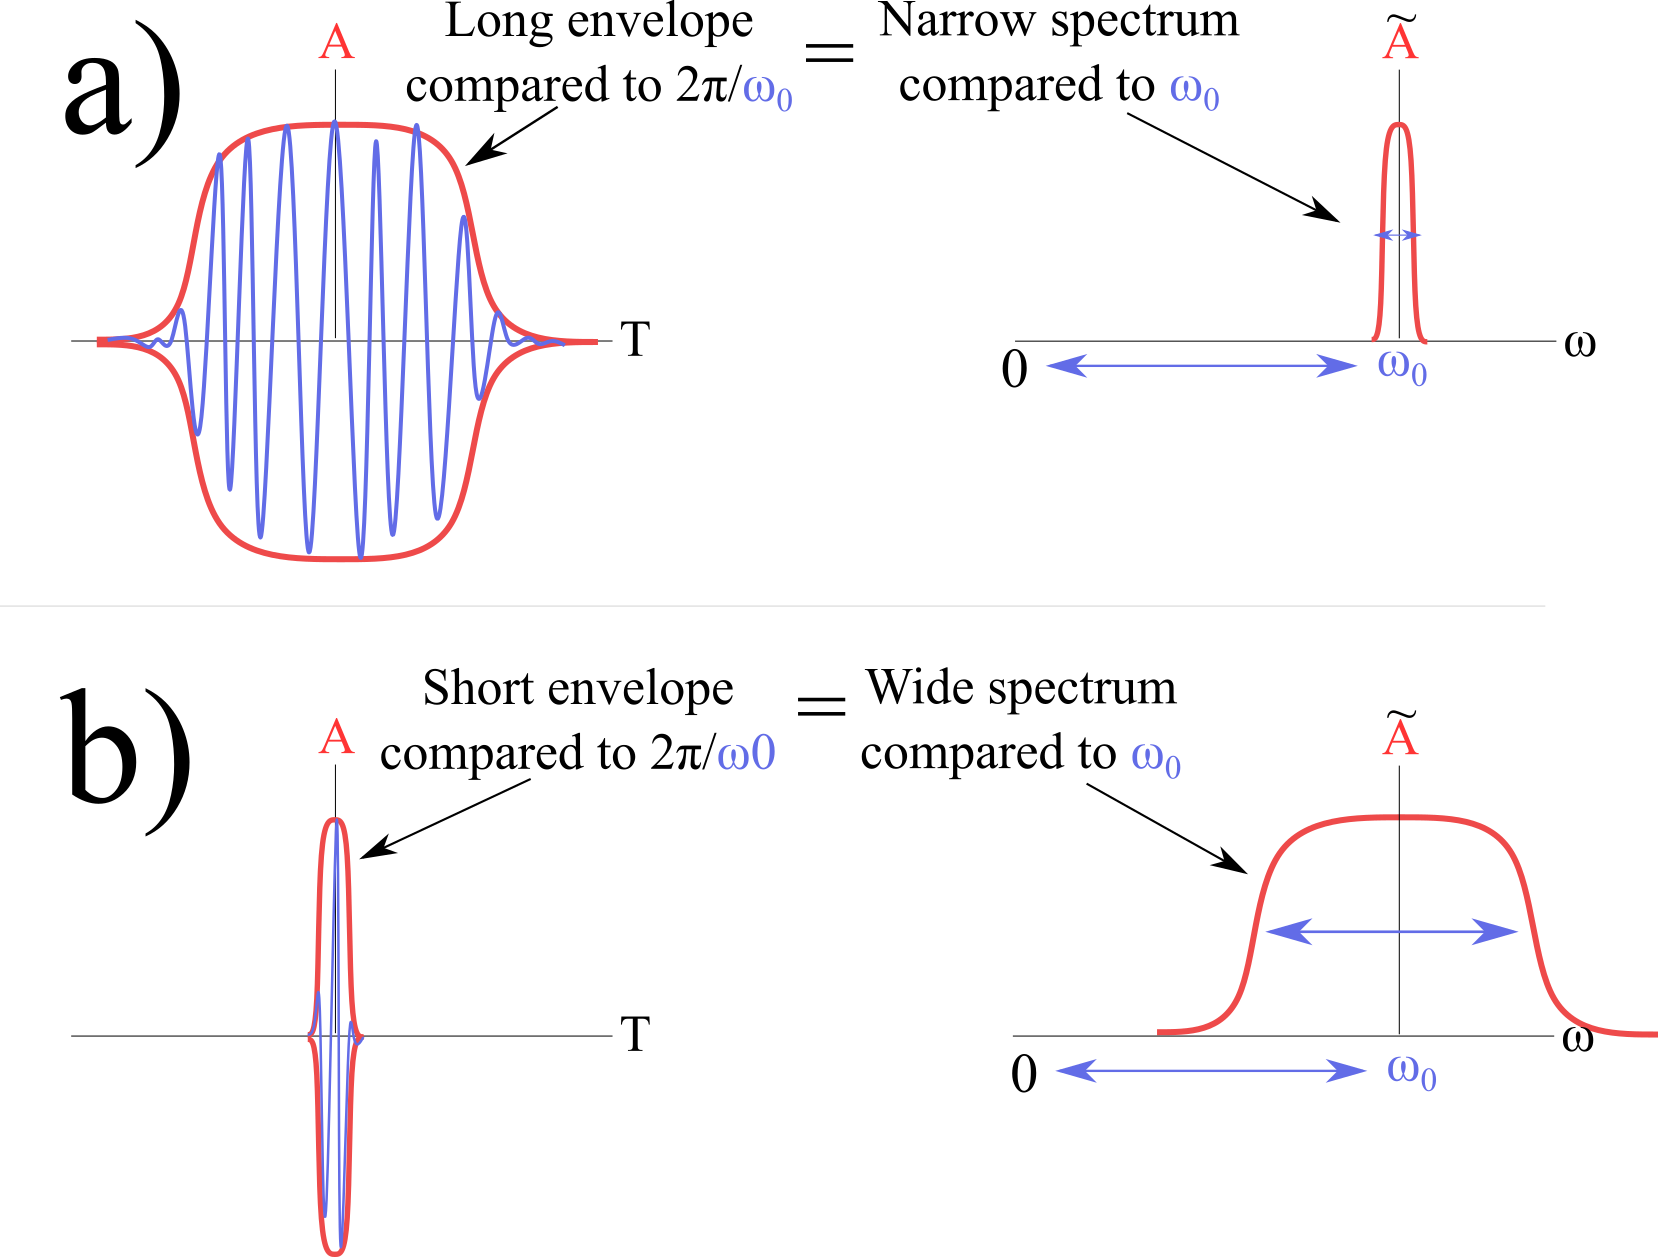
\includegraphics[width=1\linewidth]{figures/bandwidth.png}
    \caption{a) 与载波频率下单次电场振荡的持续时间相比,持续时间长的脉冲频谱较窄。 b)相反,短脉冲的频谱较宽。}
    \label{fig:bandwidth}
\end{figure}

根据这些假设,脉冲的频谱宽度非常窄,以至于 $\betag(\omega)$ 可以围绕载波频率泰勒展开为

\begin{align}
\label{eq:beta_approx}
    \betag(\omega)&\approx \betag(\omega_0)+\partial_\omega\betag|_{\omega_0}(\omega-\omega_0)+\frac{1}{2!}\partial^2_\omega\betag|_{\omega_0}(\omega-\omega_0)^2+
    \frac{1}{3!}\partial^3_\omega\betag|_{\omega_0}(\omega-\omega_0)^3+... \\ \nonumber
    &= \sum_{n=0}^{\infty} \frac{1}{n!}\partial^n_\omega\betag|_{\omega_0}(\omega-\omega_0)^n\\ \nonumber
    &=\sum_{n=0}^{\infty} \frac{1}{n!}\betag_n(\omega-\omega_0)^n.
\end{align}

考虑到这一简化,脉冲在介质中传播的表达式变为

\begin{align}
\label{eq:beta_approx_applied}
    \E(z,t) &= \frac{1}{2\pi}\int_{-\infty}^{\infty} \Tilde{\E}(z,\omega) e^{i(\betag_0+\betag_1(\omega-\omega_0)+\frac{1}{2}\betag_2(\omega-\omega_0)^2+...)z-i\omega t} d\omega.
\end{align}


\section{$\betag_0$ - 载波的延迟程度}

%Because the term containing $\betag_0$ does not depend on $\omega$, it can be moved outside the integral in Eq.~\ref{eq:beta_approx_applied}. Multiplying by $1=\exp(-i\omega_0t)\exp(i\omega_0t)$ yields
由于包含 $\betag_0$ 的项不依赖于 $\omega$,它可以移到公式 ~\ref{eq:beta_approx_applied} 的积分之外。乘以 $1=\exp(-i\omega_0t)\exp(i\omega_0t)$ 得到

\begin{align}
\label{eq:beta_approx_applied}
    \E(z,t) &= \frac{1}{2\pi} e^{i\betag_0z-i\omega_0t}  \int_{-\infty}^{\infty} \Tilde{\E}(z,\omega) e^{i(\betag_1(\omega-\omega_0)+\frac{1}{2}\betag_2(\omega-\omega_0)^2+...)z-i(\omega-\omega_0) t} d\omega.
\end{align}

积分外的指数意味着,如果观察介质中的复数电场,其持续时间为载波的几个周期,那么它看起来就像一个复数平面波,其时间频率为 $\omega_0$,空间频率为 $\betag_0$。关于 $\betag_0$ 对真实平面波在介质中传播的影响,请参见 \href{https://www.desmos.com/calculator/ausd1wnl2j}{此交互式图表}。

\subsection{相速度}
\label{sec:Phase_velocity}

当 $\betag_0z-\omega_0t$ 是 $2\pi$ 的整数倍时,载波将达到峰值。为简单起见,考虑与 $\betag_0z-\omega_0t=0$ 相对应的峰值。如果时间前进了 $0<Delta t$,$z$ 的原始值就不满足 $\betag_0z-\omega_0(t+\Delta t)=0$ 。相反,峰值会出现在某个新的位置 $z+\Delta z$,其中

\begin{align}
    \betag_0(z+\Delta z)-\omega_0(t+\Delta t)=0\\ \nonumber
    \betag_0\Delta z-\omega_0\Delta t=0.
\end{align}

由于峰值在 $\Delta t$ 时间内移动了 $\Delta z$,我们可以将 “相位速度”(或 “载波速度”)定义为

\begin{align}
\label{eq:Phase_velocity}
    v_p &= \frac{\Delta z}{\Delta t} = \frac{\omega_0}{\betag_0}.
\end{align}


\section{$\betag_1$ - 以载波为中心的脉冲包络延迟的程度}

式 ~\ref{eq:beta_approx_applied} 中的积分表示通过介质传播的复电场的包络。对指数项进行重排,可以得到

\begin{align}
\label{eq:envelope_beta1}
    \E(z,t) &= \frac{1}{2\pi} e^{i\betag_0z-i\omega_0t}  \int_{-\infty}^{\infty} \Tilde{\E}(z,\omega) e^{i\betag_1(\omega-\omega_0)z-i(\omega-\omega_0) t} e^{i(\frac{1}{2}\betag_2(\omega-\omega_0)^2+...)z} d\omega.
\end{align}

应用公式 ~\ref{eq:Phase_velocity} 后面的相同分析,我们会发现复电场包络的峰值以所谓的 “群速度”(或 “包络速度”)传播,其值为

\begin{align}
\label{eq:group_velocity}
    v_g &= \frac{(\omega-\omega_0)}{\betag_1\cdot(\omega-\omega_0)} = \frac{1}{\betag_1} = \frac{1}{\partial_\omega\betag}.
\end{align}

关于相位速度和群速度之间的区别,请参见 \href{https://www.desmos.com/calculator/rq2physwac}{此交互式图表}。请注意,公式~\ref{eq:group_velocity}与公式~\ref{eq:delay_definition}的预测一致,即相位相对于 $\omega$ 发生较大的正向变化应导致较大的延迟。




\section{$\betag_2$ - 构成以载波为中心的脉冲包络的频率相对延迟的程度}

\label{sec:GVD}

将公式 ~\ref{eq:envelope}应用于公式 ~\ref{eq:envelope_beta1},可以 “剔除 ”载波快速但可预测的空间和时间振荡,将注意力集中在包络上:

\begin{align}
    \A(z,t)  &= \frac{1}{2\pi}  \int_{-\infty}^{\infty} \Tilde{\A}(z,\omega) e^{i\betag_1(\omega-\omega_0)z-i(\omega-\omega_0) t} e^{i(\frac{1}{2}\betag_2(\omega-\omega_0)^2+...)z} d\omega.
\end{align}

为了进一步简化,我们可以定义 $T=t-\betag_1z$,即 “脉冲包络到达距离 $z$ 时的相对时间”。使用 $T$ 代替 $t$ 是很方便的,因为许多光学实验都需要发送脉冲光穿过固定长度的介质,并跟踪光离开介质后一段时间内测量到的功率:   

\begin{align}
    \A(z,T)  &= \frac{1}{2\pi}  \int_{-\infty}^{\infty} \Tilde{\A}(z,\omega) e^{i\betag_1(\omega-\omega_0)z-i(\omega-\omega_0) (T+\betag_1z)} e^{i(\frac{1}{2}\betag_2(\omega-\omega_0)^2+...)z} d\omega \\ \nonumber
    &= \frac{1}{2\pi}  \int_{-\infty}^{\infty} \Tilde{\A}(z,\omega) e^{i(\frac{1}{2}\betag_2(\omega-\omega_0)^2+...)z-i(\omega-\omega_0)T} d\omega.
\end{align} 

正如公式 ~\ref{eq:spectrum_time_example}所解释的那样,$\betag_2$ 的正值(负值)意味着较低的(较高的)时间频率比较高的(较低的)时间频率传播得更快,从而导致脉冲包络在时域中变宽。或者,我们也可以考虑只包含 $\betag_2$ 项的公式 ~\ref{eq:GNLSE}、

\begin{align}
    \label{eq:heat_equation}
    \partial_z \A = -i  \frac{\betag_2}{2}\partial_T^2\A,
\end{align}

这与所谓的 “热方程 ”相同 ~\cite{Fourier_heat_original,Fourier_heat_english}. 参见 
\href{https://digitalcommons.ursinus.edu/cgi/viewcontent.cgi?article=1008&context=triumphs_differ}{本教程}。为了得到 $\A(z,T)$ 给定的 $\A(z=0,T)$ 以及 $\tilde{A}(z=0,\omega)$ ,首先计算公式的傅立叶变换 ~\ref{eq:heat_equation} 以得到

\begin{align}
    \label{eq:beta2_broadening}
    \partial_z \Tilde{\A} &= -i  \frac{\betag_2}{2} (i(\omega-\omega_0))^2 \Tilde{\A} \\ \nonumber
    &= i  \frac{\betag_2}{2}(\omega-\omega_0)^2\Tilde{\A} \\ \nonumber
    \Tilde{\A}(z,\omega)&=\Tilde{\A}(0,\omega)e^{i\frac{\betag_2}{2}(\omega-\omega_0)^2z} \\ \nonumber
    \A(z,T) &= \IFT\left\{  \Tilde{\A}(z,\omega)   \right\}.
\end{align}

对于高斯脉冲,公式(~\ref{eq:beta2_broadening})可以通过(\href{https://drive.google.com/file/d/17Ab3bg0Hx0x8J-5lR29ejFg0eOlv6Psh/view?usp=sharing}{分析})求解。结果确实意味着脉冲会在时间上变宽,而将公式\ref{eq:chirp_definition}应用于结果则证实,$\betag_2>0$ 意味着低频将比高频更早到达。由于$\betag_2$引起的相位偏移的大小随着给定频率分量与载波之间距离的增加而呈二次增长,因此在相同距离内,频谱宽度较大的短脉冲将比带宽较小的短脉冲在时间上更宽。由 $\betag_2$ 导致的增宽变得显著的特征长度可定义为

\begin{align}
    \label{eq:Dispersion_length}
    L_{2} &= \frac{T_0^2}{|\betag_2|}.
\end{align}

有关色散对高斯脉冲的影响,请参阅 \href{https://www.youtube.com/watch?v=BP6Ra98AEuU}{本视频}。

\subsection{零色散频率}
\label{subsec:ZDF}

对于已知 $\betag(\omega)$ 的给定介质,可以计算出给定载波频率 $\omega_0$ 附近的 $\betag_2$ 值为

\begin{align}
\label{eq:ZDF}
    \betag_2(\omega) &= \betag_2|_{\omega=\omega_0} + \betag_3|_{\omega=\omega_0}\cdot(\omega-\omega_0)+\frac{1}{2}\betag_4|_{\omega=\omega_0}\cdot(\omega-\omega_0)^2 +...,
\end{align}

这样就可以求解特定频率(或者说复数频率!),$\omega_{ZD}$,其中$\betag_2(\omega_{ZD})=0$。这个 “零色散频率 ”非常重要,因为很多非线性机制在 $\omega_{ZD}$ 或接近 $\omega_{ZD}$ 的频率下会更有效,其中 $\betag_2<0$。因此,在进行非线性光学实验时,确定特定介质的 $\omega_{ZD}$ 值至关重要。特定光纤的零色散频率可以使用常见的光学实验室设备进行实验测量~\cite{zero_disp_measurement}。
从历史上看,用于电信的光纤被设计成接近激光的近红外频率($\approx$190-230~THz $\approx$1310-1550~nm),易于产生、调制和检测。这样做的目的是为了防止携带数字信息的脉冲出现时间展宽、重叠和干扰。自 2000 年代中期以来,电子色散补偿技术的进步使这种光纤设计变得过时甚至有害,因为非线性效应会通过改变信号的相位和振幅来扭曲信号,在接近 $\omega_{ZD}$ 时这种效应更为显著。

\section{$\betag_n$ - 高阶延迟}

在理解了$\betag(\omega)$(即$\betag_1$)的斜率决定脉冲包络的传播速度,而$\betag(\omega)$(即$\betag_2$)的曲率决定脉冲的时间展宽之后,这些见解可以得到推广。例如,$\betag_3>0$ 意味着$i\betag_3/6(\omega-\omega_0)^3z$ 项会导致除载波外所有频率的正$\partial_\omega\phi$。因此,对脉冲有贡献的高频和低频都会开始落后于主脉冲,从而导致不对称的时间展宽。此外,$\betag_4>0$意味着$i\betag_4/24(\omega-\omega_0)^4z$会在$\betag_2$引起的时间展宽之外引起额外的对称时间展宽。请参见图 ~\ref{fig:dispersion_combined},了解不同的 $\betag_n$ 项对高斯脉冲时间轮廓的影响。在分析脉冲在介质中传播的演化时,$\betag(\omega)$ 的扩展中包含多少项取决于脉冲的频谱宽度,而频谱宽度与其持续时间成反比。对于 1~ps 以上的脉冲,高于 $\betag_3$ 的阶数很少有贡献。在用持续时间为 10~fs 的脉冲对超连续产生进行数值模拟时,为了稳妥起见,通常会包含高达 $\betag_8$ 的阶次。与公式~\ref{eq:Dispersion_length}类似,高阶色散效应变得显著的特征长度定义为

\begin{align}
\label{eq:dispersion_length_general}
    L_{n} &= \frac{T_0^n}{|\betag_n|}.
\end{align}

有关色散的更多详情,请参阅 \href{https://www.youtube.com/watch?v=E3S0BQiy3p8&ab_channel=YourFavouriteTA}{本视频教程}。


\section{$\alpha(\omega)$ 和 $\betag(\omega)$ 是独立的吗?}
\label{sec:KK_relations}

在公式~\ref{eq:GNLSE}中,$\alpha$被视为常数,因为在典型脉冲的带宽范围内,其频率依赖性通常很弱。然而,原则上我们可以像对待 $\betag(\omega)$ 一样,对 $\alpha(\omega)$ 进行泰勒展开。有趣的是,我们发现对于给定介质来说,函数 $\alpha(\omega)$ 和 $\betag(\omega)$ 是通过所谓的 \href{https://en.wikipedia.org/wiki/Kramers%E2%80%93Kronig_relations#Related_proof_from_the_time_domain}{克莱默斯-克罗尼格关系(Kramers-Kronig Relations)} 相互关联的,知道其中一个就可以计算另一个。因此,$\alpha(\omega)$ 和 $\betag(\omega)$ 不能独立选择。从数学上证明这种联系很困难,但从物理上来说,直觉告诉我们,与频率相关的$\alpha(\omega)$吸收从根本上说正是产生与频率相关的相位延迟$\betag(\omega)$的原因。此外,介质在给定位置对外加电场的响应只能取决于该位置电场的当前和过去的值,这进一步限制了衰减和相位延迟的组合。方便的是,如果将 $\alpha(\omega)=\alpha$ 视为频率常数,那么它的值可以自由改变,而不会影响 $\betag_n$ 的任何值。 

有关克拉默-克罗尼格关系的更多详情,请参见 \href{https://www.youtube.com/watch?v=vzBnsG2rKWs}{视频一 } 和 \href{https://www.youtube.com/watch?v=rFTUTxPHYYw}{视频二}。请参阅 \href{https://www.desmos.com/calculator/1zymtgbbrv}{这个交互图},了解在时域中使用因果关系和克拉默-克罗尼格关系将 $\alpha(\omega)$ 与 $\betag(\omega)$ 联系起来的教程。


\begin{figure}
    \centering
    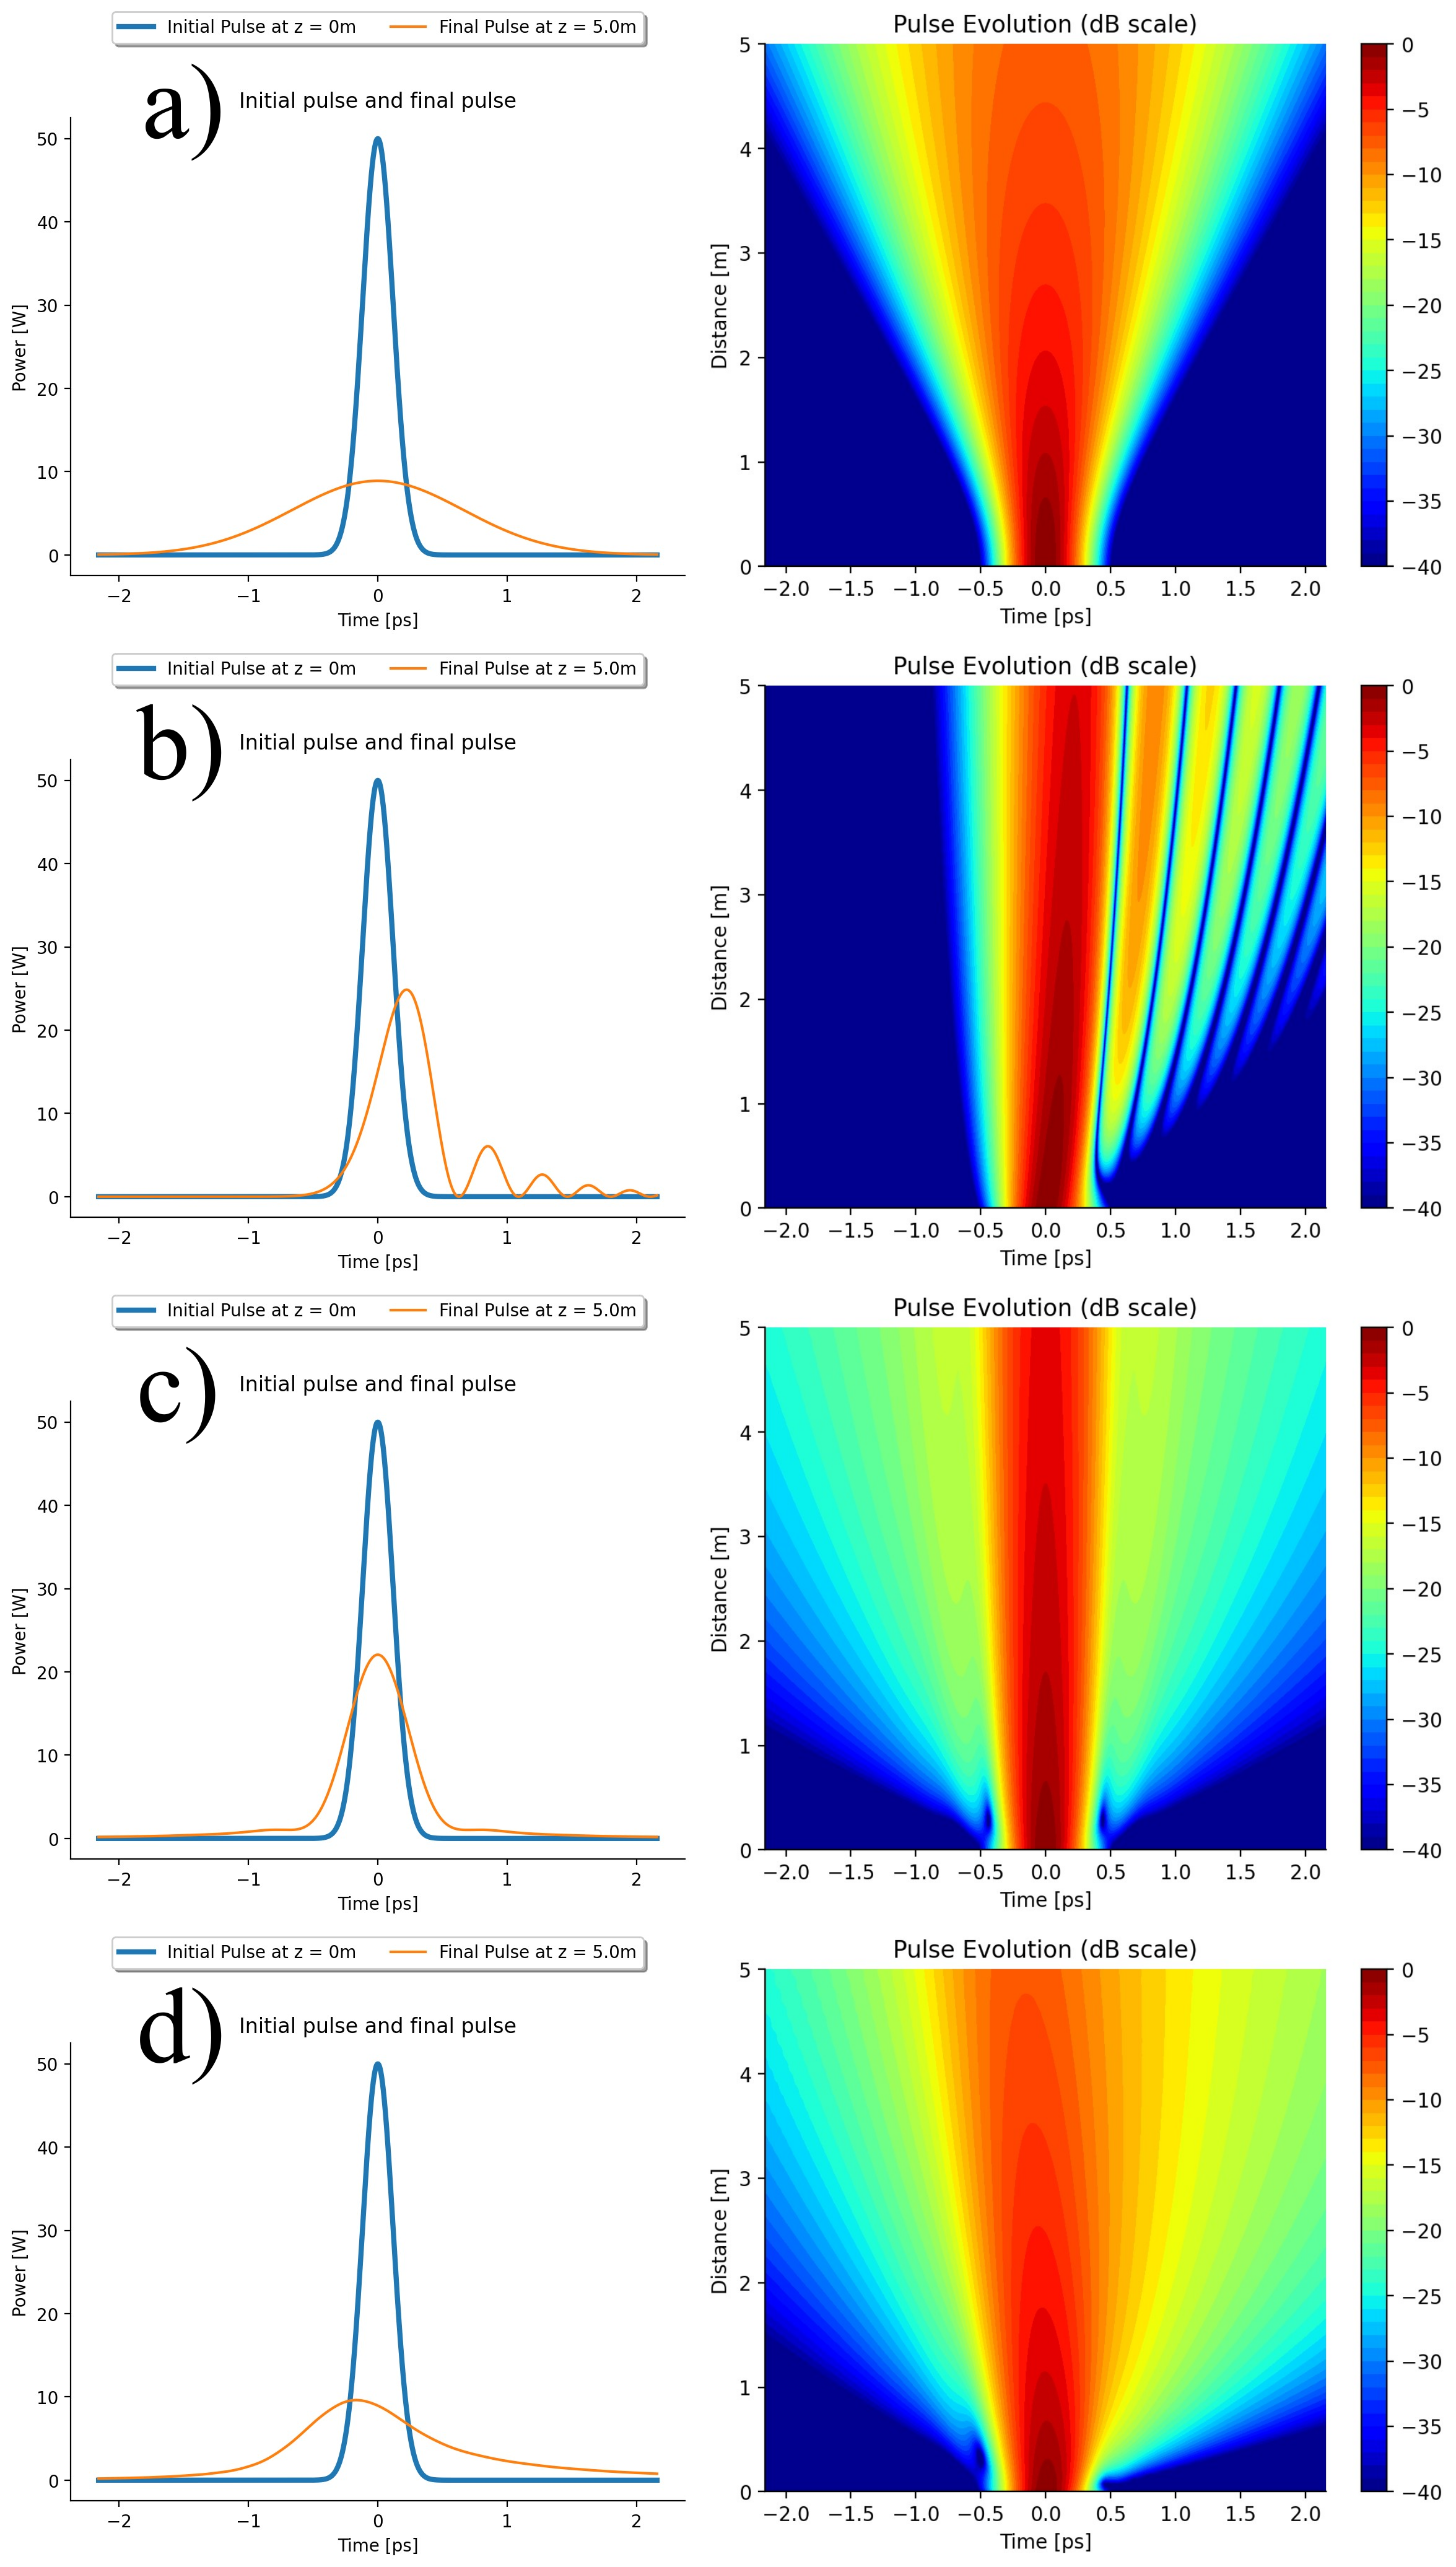
\includegraphics[width=0.75\linewidth]{figures/dispersion_combined.png}
    \caption{时域中不同 $\betag_n$ 项对高斯脉冲的影响说明。左栏显示了脉冲在不同$\betag_n$项介质中传播前后的功率包络对比。右栏显示的是功率包络随距离的变化。  a) $\betag_2<0$ 的介质; b) $\betag_3>0$ 的介质; c) $\betag_4<0$ 的介质; d) 同时存在 $\betag_2<0$ 、 $\betag_3>0$ 和 $\betag_4<0$ 的介质。
    使用 \href{https://colab.research.google.com/drive/1PW9smFA3PECvcXyWpZcW1ogY4W3hEYFt?usp=sharing}{这个可交互notebook} 中的数值模拟生成。我们鼓励读者尝试使用。}
    \label{fig:dispersion_combined}
\end{figure}
    \chapter{自相位调制}
\label{ch:SPM}

在具有三阶非线性的材料中,某一时刻的折射率取决于该时刻的光功率。因此,与低功率但形状相同的脉冲相比,高功率脉冲将经历更大的相位变化。由于非线性介质中可以同时存在不同频率的光,描述非线性对光场的影响可能较为复杂。本章解释了一个简单的情况,即“自相位调制”(SPM),其中仅存在一个以单一载频为中心的脉冲。

\section{脉冲中的相位变化}
从方程~\ref{eq:GNLSE}出发,并假设除$\gamma>0$之外的所有参数都为零,$\omega_0\A\gg\partial_T\A$,且$R(T_{delay})=\delta(T_{delay})$,则广义非线性薛定谔方程简化为
\begin{align}
\label{eq:SPM}
    \partial_z\A &= i\gamma|\A|^2\A.
\end{align}
从数学角度看,方程~\ref{eq:SPM}表明,对于$z$的微小变化,复数$\A$的变化量等于其自身在复平面上旋转90度($i\A$),并根据其自身的平方模($|\A|^2$)以及标量$\gamma$进行缩放。从物理角度看,方程~\ref{eq:SPM}暗示非线性效应会根据功率改变场的瞬时相位,但不会改变该瞬时的功率大小。解方程~\ref{eq:SPM}得到
\begin{align}
    \label{eq:SPM_applied}
    \A(z,T)&= \A(0,T)\exp\left( i\gamma|\A(0,T)|^2z \right).
\end{align}
为了理解方程~\ref{eq:SPM_applied}的含义,可以参考方程~\ref{eq:chirp_definition},该方程指出脉冲的瞬时频率与其相位相对于时间的负导数有关。假设一个高斯脉冲$\A(0,T)=\A_0\exp(-T^2/2T_0^2)$,则该脉冲在通过非线性介质传播距离$z$后的瞬时频率为
\begin{align}
\label{eq:SPM_example}
    \delta\omega(z,T) &= -\gamma |\A_0|^2 z\partial_T \exp\left(-\frac{T^2}{T_0^2}\right)\\ \nonumber
    &= 2\gamma |\A_0|^2 z T/T_0^2 \exp\left(-\frac{T^2}{T_0^2}\right),
\end{align}
这表明脉冲前沿将产生红移,后沿将产生蓝移。参见图~\ref{fig:chirp_profiles}(a)以了解高斯脉冲产生的啁啾可视化,参见图~\ref{fig:chirp_profiles}(b-d)以了解其他脉冲形状产生的啁啾。考虑方程~\ref{eq:SPM_applied}中指数的参数,可定义非线性效应变得显著的特征长度为
\begin{align}
    L_{NL} &= \frac{1}{\gamma P_0} = \frac{1}{\gamma |\A(0,T)|^2},  
\end{align}
其中$P_0$为脉冲的初始峰值功率。

\begin{figure}
    \centering
    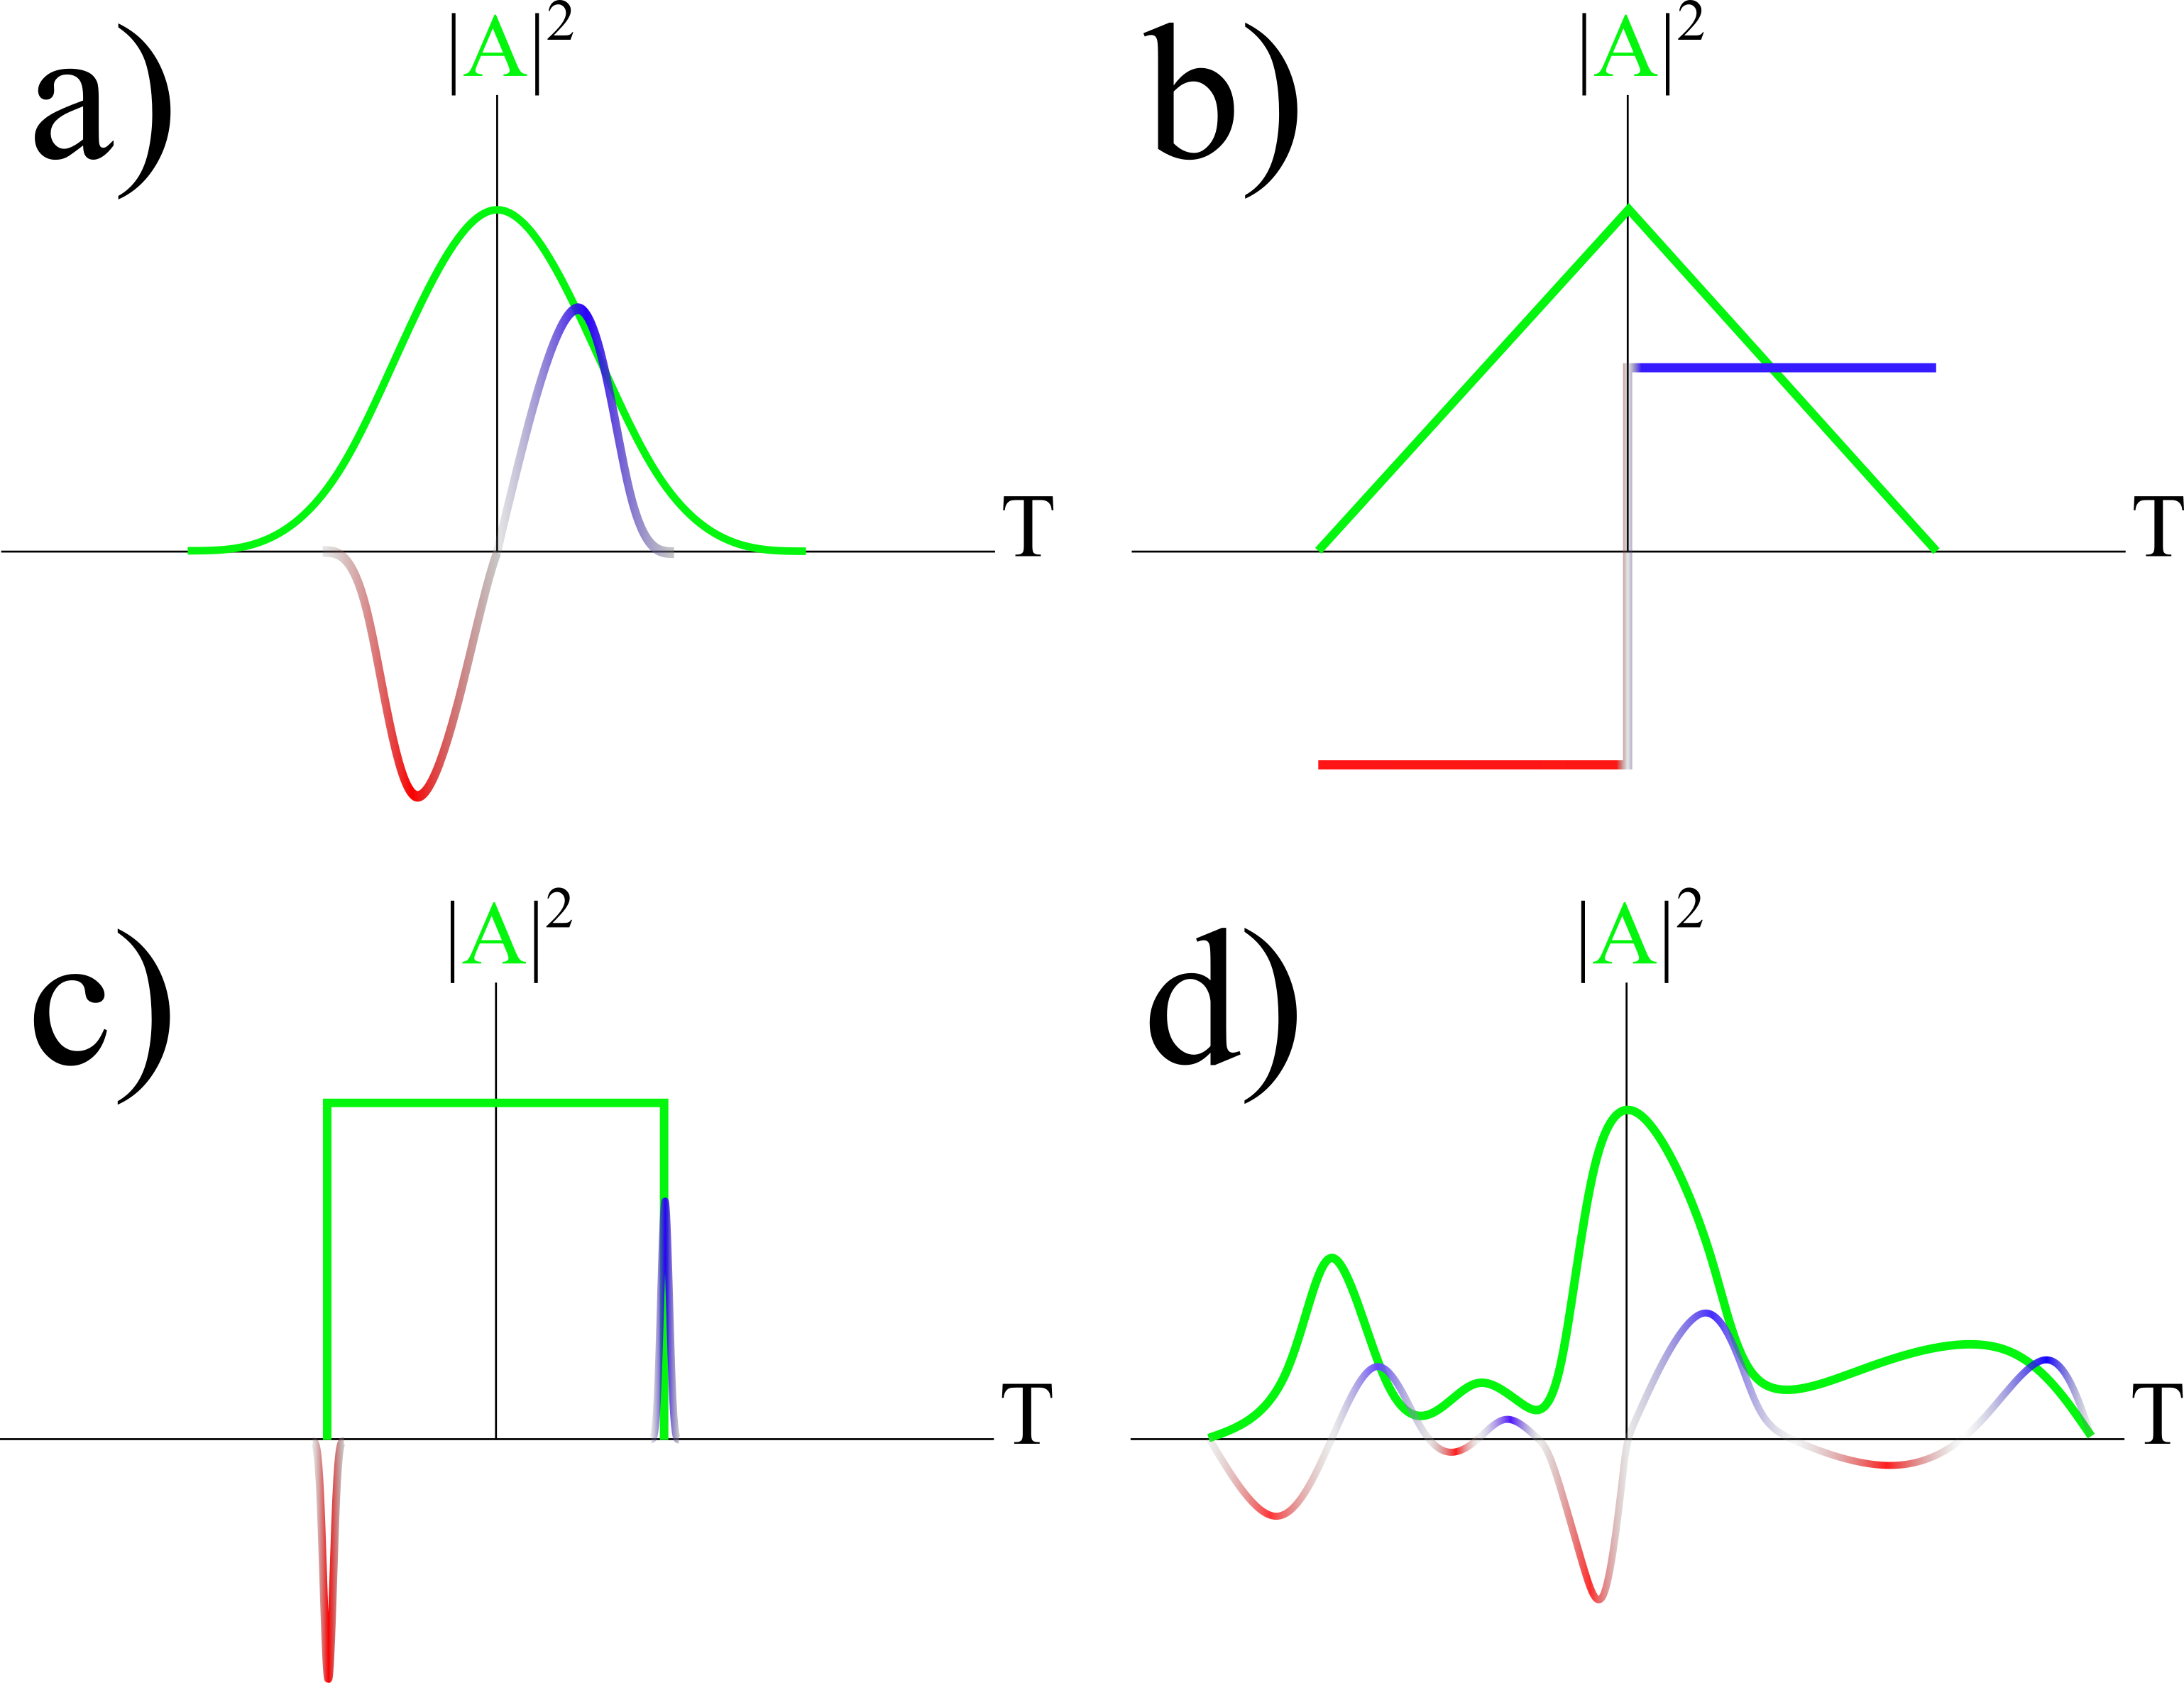
\includegraphics[width=0.75\linewidth]{figures/SPM_chirp.png}
    \caption{SPM对(a)高斯脉冲,(b)三角脉冲,(c)方波脉冲,(d)任意脉冲的影响可视化。一般来说,正斜率会导致红移啁啾,负斜率导致蓝移啁啾,水平斜率则不会产生啁啾。}
    \label{fig:chirp_profiles}
\end{figure}

\section{谱展宽}
对等式~\ref{eq:SPM_example}的分析表明,自相位调制(SPM)会导致脉冲在前导坡度上变得“更红”,在后导坡度上变得“更蓝”。单独考虑时,$\betag_2>0$也会导致类似的行为,但关键区别在于,色散仅改变不同频率分量的相对相位,而SPM还会改变它们的幅度。换句话说,作用在脉冲上的SPM会产生新的颜色,这些颜色在最初并不存在!通过对等式~\ref{eq:SPM}两边进行傅里叶变换可以从数学上看到,这意味着在频谱域中的展宽,因为傅里叶变换在时域中两个函数的乘积等效于频域中的卷积:

\begin{align}
\label{eq:SPM_freq}
    \partial_z\Tilde{\A} &= i\gamma \FT\left\{\A\A^*\A\right\} \\ \nonumber
    &= i\gamma \Tilde{\A}*\Tilde{\A^*}*\Tilde{\A}.
\end{align}

简而言之,等式~\ref{eq:SPM_freq} 表明 $\A$ 的频谱相对于 $z$ 的变化取决于其频谱与自身及其复共轭的卷积。由于卷积两个函数会产生一个比初始函数更宽的函数,等式~\ref{eq:SPM_freq}显示频谱将随距离的增加而展宽,暗示通过将功率从载波向红、蓝端转移而添加新频率。请参见图~\ref{fig:SPM_before_and_after},了解SPM对高斯脉冲的影响示例。

\begin{figure}
    \centering
    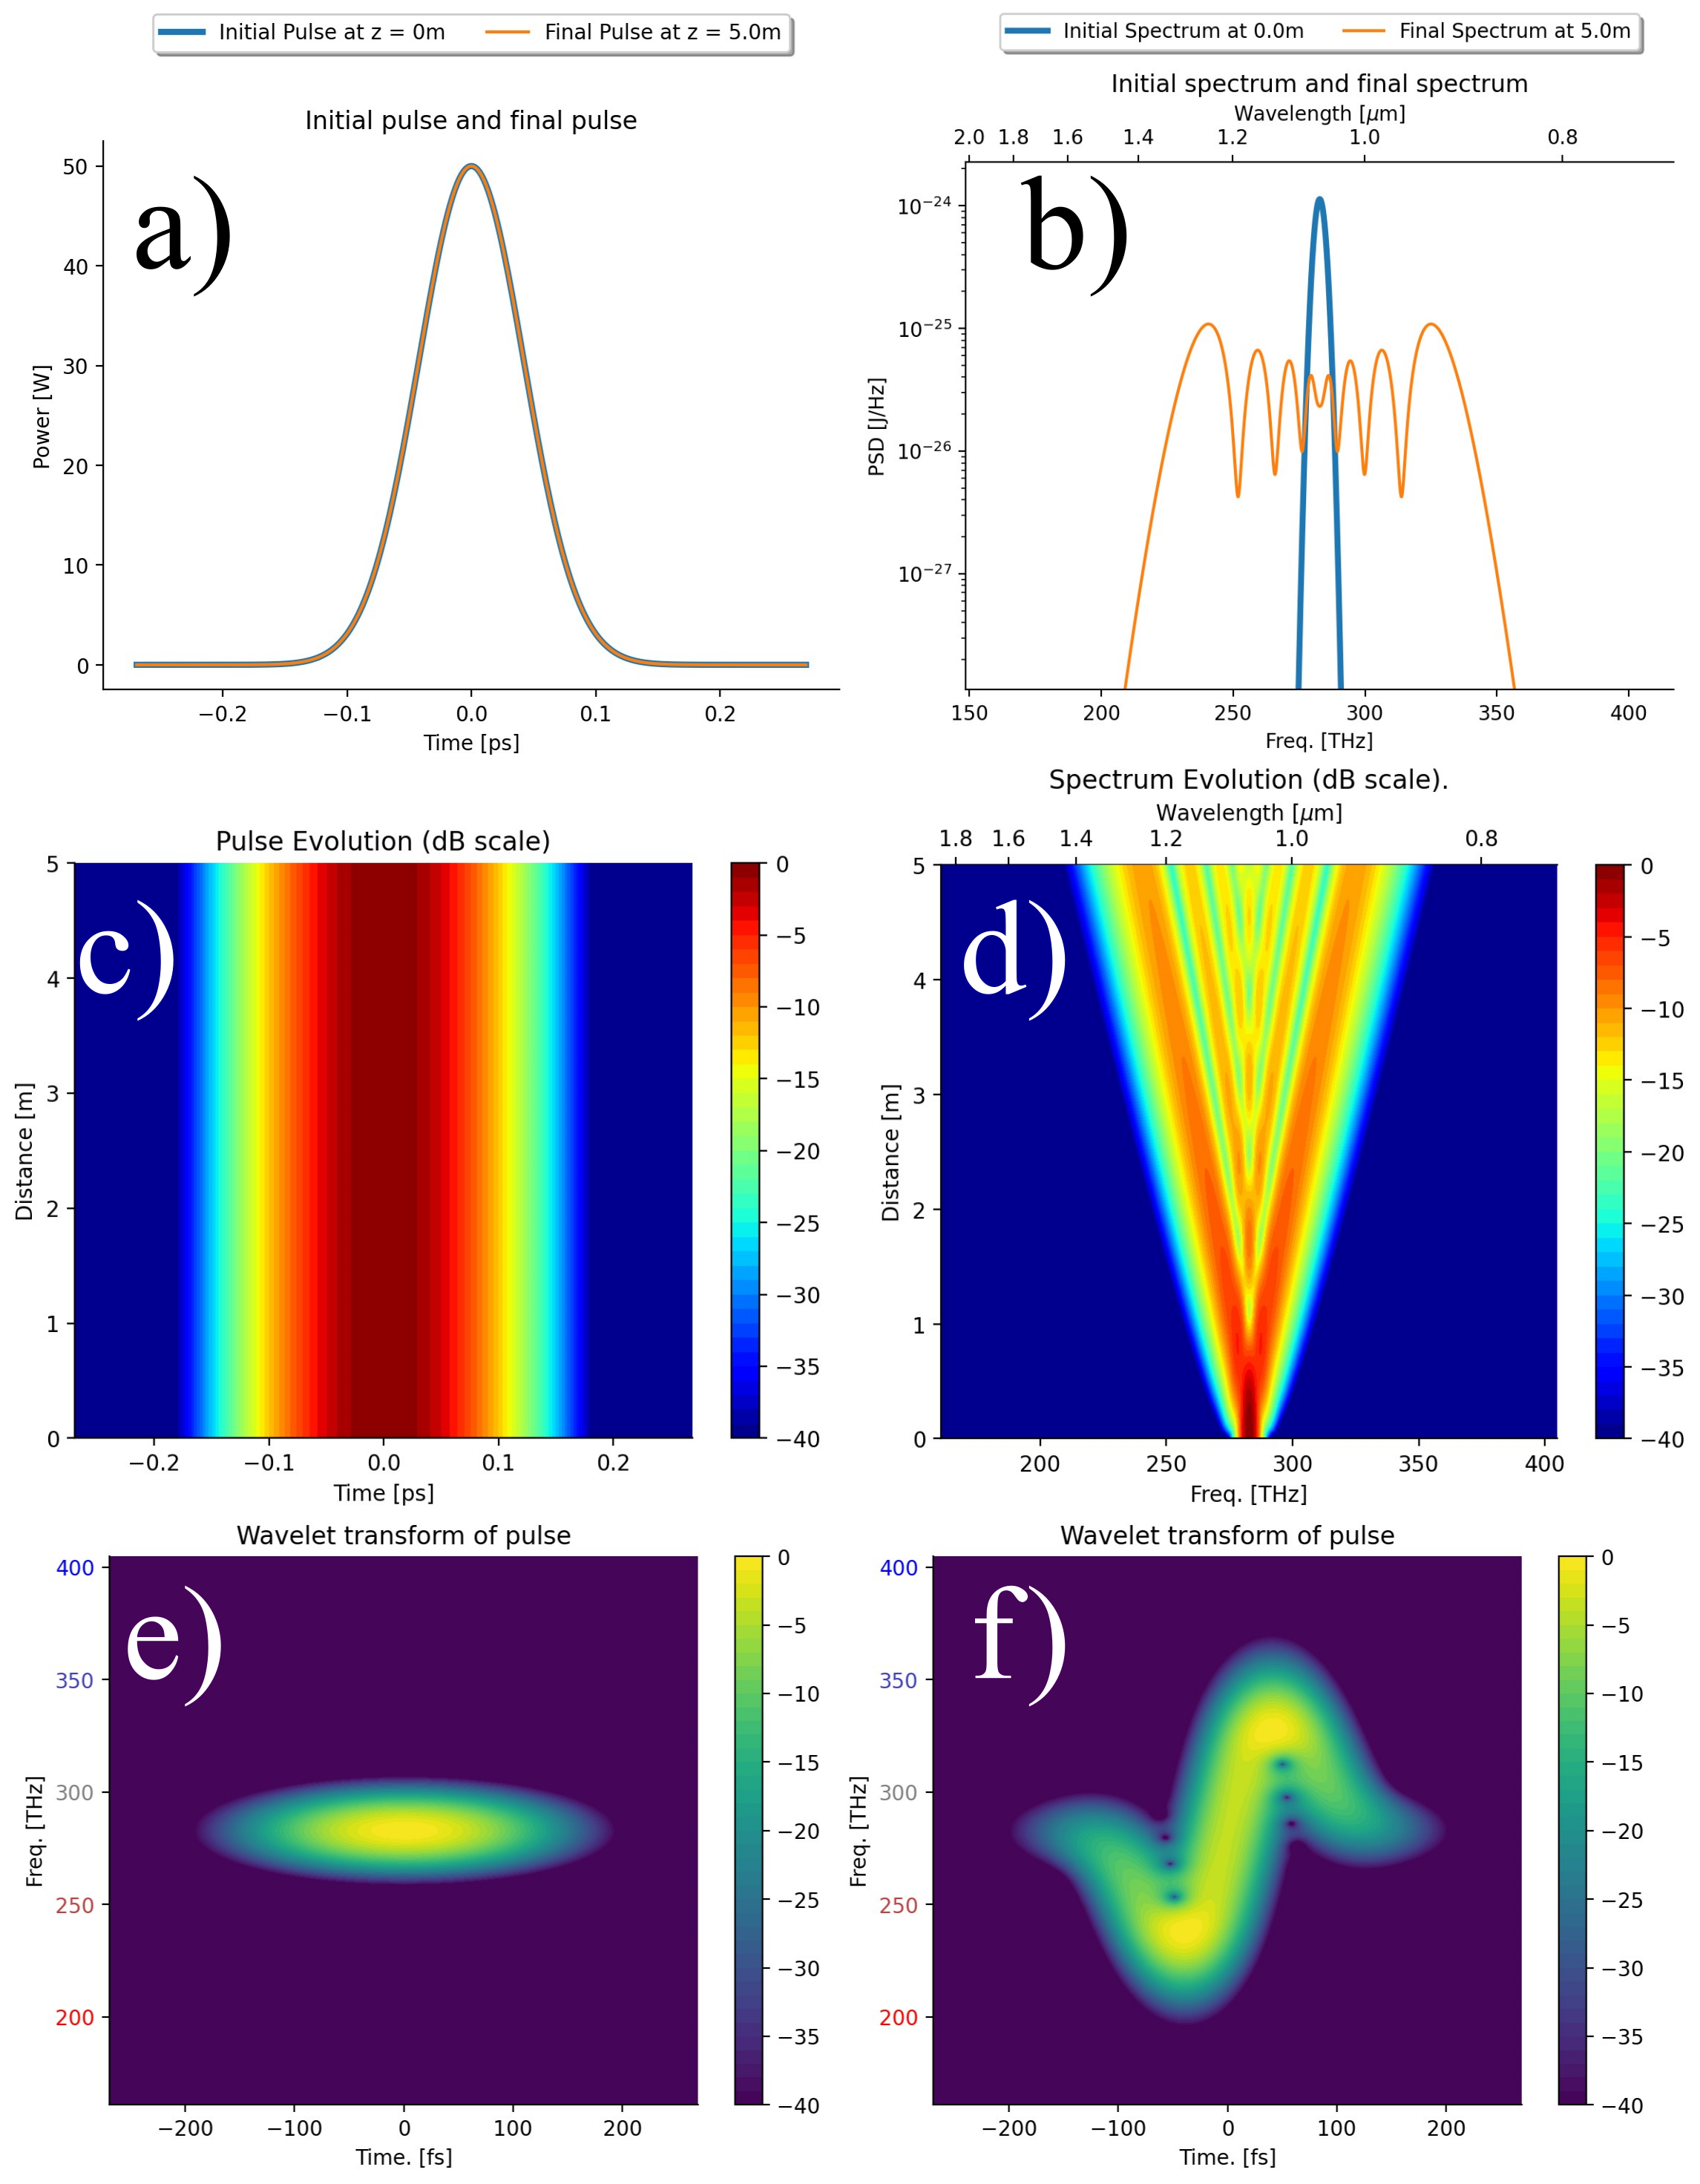
\includegraphics[width=1\linewidth]{figures/SPM_combined.png}
    \caption{ 高斯脉冲在由等式~\ref{eq:SPM}描述的非线性介质中传播的前后对比。
    a) 在时域中,脉冲的功率包络保持不变。 b) 频谱展宽。 c) 时域中功率包络的演化没有变化。 d) 频谱逐渐展宽。 e) 传播前的脉冲频谱图。 f) 传播后的脉冲频谱图。请注意频谱域中的展宽以及时间域中宽度的恒定。使用\href{https://colab.research.google.com/drive/1P41F4hO6Mv12RsEkpogYv5teQyFZ6iW0?usp=sharing}{这个交互notebook}中的数值模拟生成图形,读者可以尝试进行实验。}
    \label{fig:SPM_before_and_after}
\end{figure}


\section{自相位调制、损耗与“有效长度”}
考虑等式~\ref{eq:GNLSE},假设与等式~\ref{eq:SPM}相同,但此时 $\alpha\neq0$。回忆等式~\ref{eq:attenuation_power},其中 $\alpha\neq0$ 会导致脉冲功率随距离呈指数变化。在这种情况下,

\begin{align}
\label{eq:SPM_and_loss}
    \partial_z\A &= \frac{\alpha}{2}\A +i\gamma|\A|^2\A\\ \nonumber
    &=\left(\frac{\alpha}{2} +i\gamma |\A(0,T)|^2 \exp(\alpha z) \right)\A. 
\end{align}

将等式~\ref{eq:SPM_and_loss} 从 $0$ 积分到 $z$ 得到:

\begin{align}
    \label{eq:Leff_derivation}
    \A(z,T)&=\A(0,T) \exp\left( \frac{\alpha}{2}z+i\gamma|\A(0,T)|^2 \int_0^z \exp(\alpha\xi) d\xi  \right) \\ \nonumber
    &=\A(0,T) \exp\left( \frac{\alpha}{2}z+i\gamma|\A(0,T)|^2  \frac{\exp(\alpha z)-1}{\alpha}   \right) \\ \nonumber
    \A(L,T)&=\A(0,T) \exp\left( \frac{\alpha}{2}z+i\gamma|\A(0,T)|^2  L_{eff}   \right),
\end{align}

其中,具有实际长度 $L$ 的介质的“有效长度”定义为:

\begin{align}
\label{eq:L_eff}
    L_{eff}= \frac{\exp(\alpha L)-1}{\alpha}.
\end{align}

等式~\ref{eq:Leff_derivation} 和等式~\ref{eq:L_eff}提供的见解是,尽管通过让光在更长的介质中传播通常会增强非线性效应,但该介质的损耗最终会使光功率降低到所有非线性效应变得可以忽略的程度。例如,对于典型的100公里长单模光纤(损耗系数为$\alpha=-0.22$dB/km),其有效长度约为19.6公里。换句话说,光信号在100公里有损耗光纤中的非线性相移累积量大致等于在19.6公里无损耗光纤中的累积量。请参见\href{https://www.desmos.com/calculator/g6dadbxq33}{这个互动图表}以查看有效长度如何依赖于 $\alpha$。注意,当 $\alpha L\ll 1$ 时,$L_{eff}\approx L$;而在 $\alpha>0$ 的情况下(如在光放大器中),可能出现 $L_{eff}>L$。此外,$\alpha$ 在特殊的非均匀光纤或存在拉曼放大时可能随 $z$ 而变化,此时需要相应修改等式~\ref{eq:attenuation} 和等式~\ref{eq:SPM_and_loss}。

\section{自陡效应}
\label{sec:SS}

在等式~\ref{eq:SPM}中,假设非线性相位偏移与场包络乘以其平均功率成正比,即 $\A|\A|^2$。这种假设可以视为非线性响应的相对于时间的零阶泰勒近似,类似于将 $\exp(x)\approx 1$ 用于非常小的 $x$。若进一步假设场包络的变化率乘以其平均功率 $\partial_T(\A|\A|^2)$ 也有贡献,则得到:

\begin{align}
\label{eq:SS}
    \partial_z\A &= i\gamma\left(1+\frac{i}{\omega_0}\partial_T \right)\A|\A|^2.
\end{align}

在等式~\ref{eq:SS}中的括号内,第一个项是自相位调制(SPM),而第二个项称为“自陡效应”(SS)。物理上,可以理解为非线性效应导致脉冲高功率部分的折射率发生显著变化。较高的折射率意味着光传播速度更慢,因此高功率脉冲的峰值在传播时比较低强度部分减速,从而在后续时间上积累功率,导致坡度陡降。类似地,一辆大且不流线型的卡车在遇到强逆风时会比流线型汽车大幅减速,从而在后方形成堵塞,而前方交通则较稀疏。由于SS效应平坦化了脉冲前端的功率坡度,并使后端变得陡峭,因此优先将脉冲频谱蓝移,因为 $\delta\omega\propto -\partial_T|\A|^2$。请参见图~\ref{fig:SS},了解SS对与图~\ref{fig:SPM_before_and_after}相同高斯脉冲的影响。对于仅受SPM和自陡效应影响的高斯脉冲,\href{https://prefetch.eu/know/concept/self-steepening/}{可以证明}其后坡在距离

\begin{align}
    L_{SS} &= \frac{T_0\omega_0\exp(1/2)}{3\sqrt{2}\gamma P_0}
\end{align}

处变得无限陡。

更多关于SS的信息,请参考\href{https://youtu.be/Fr6yLtGZ2To}{这个视频教程}。

\begin{figure}
    \centering
    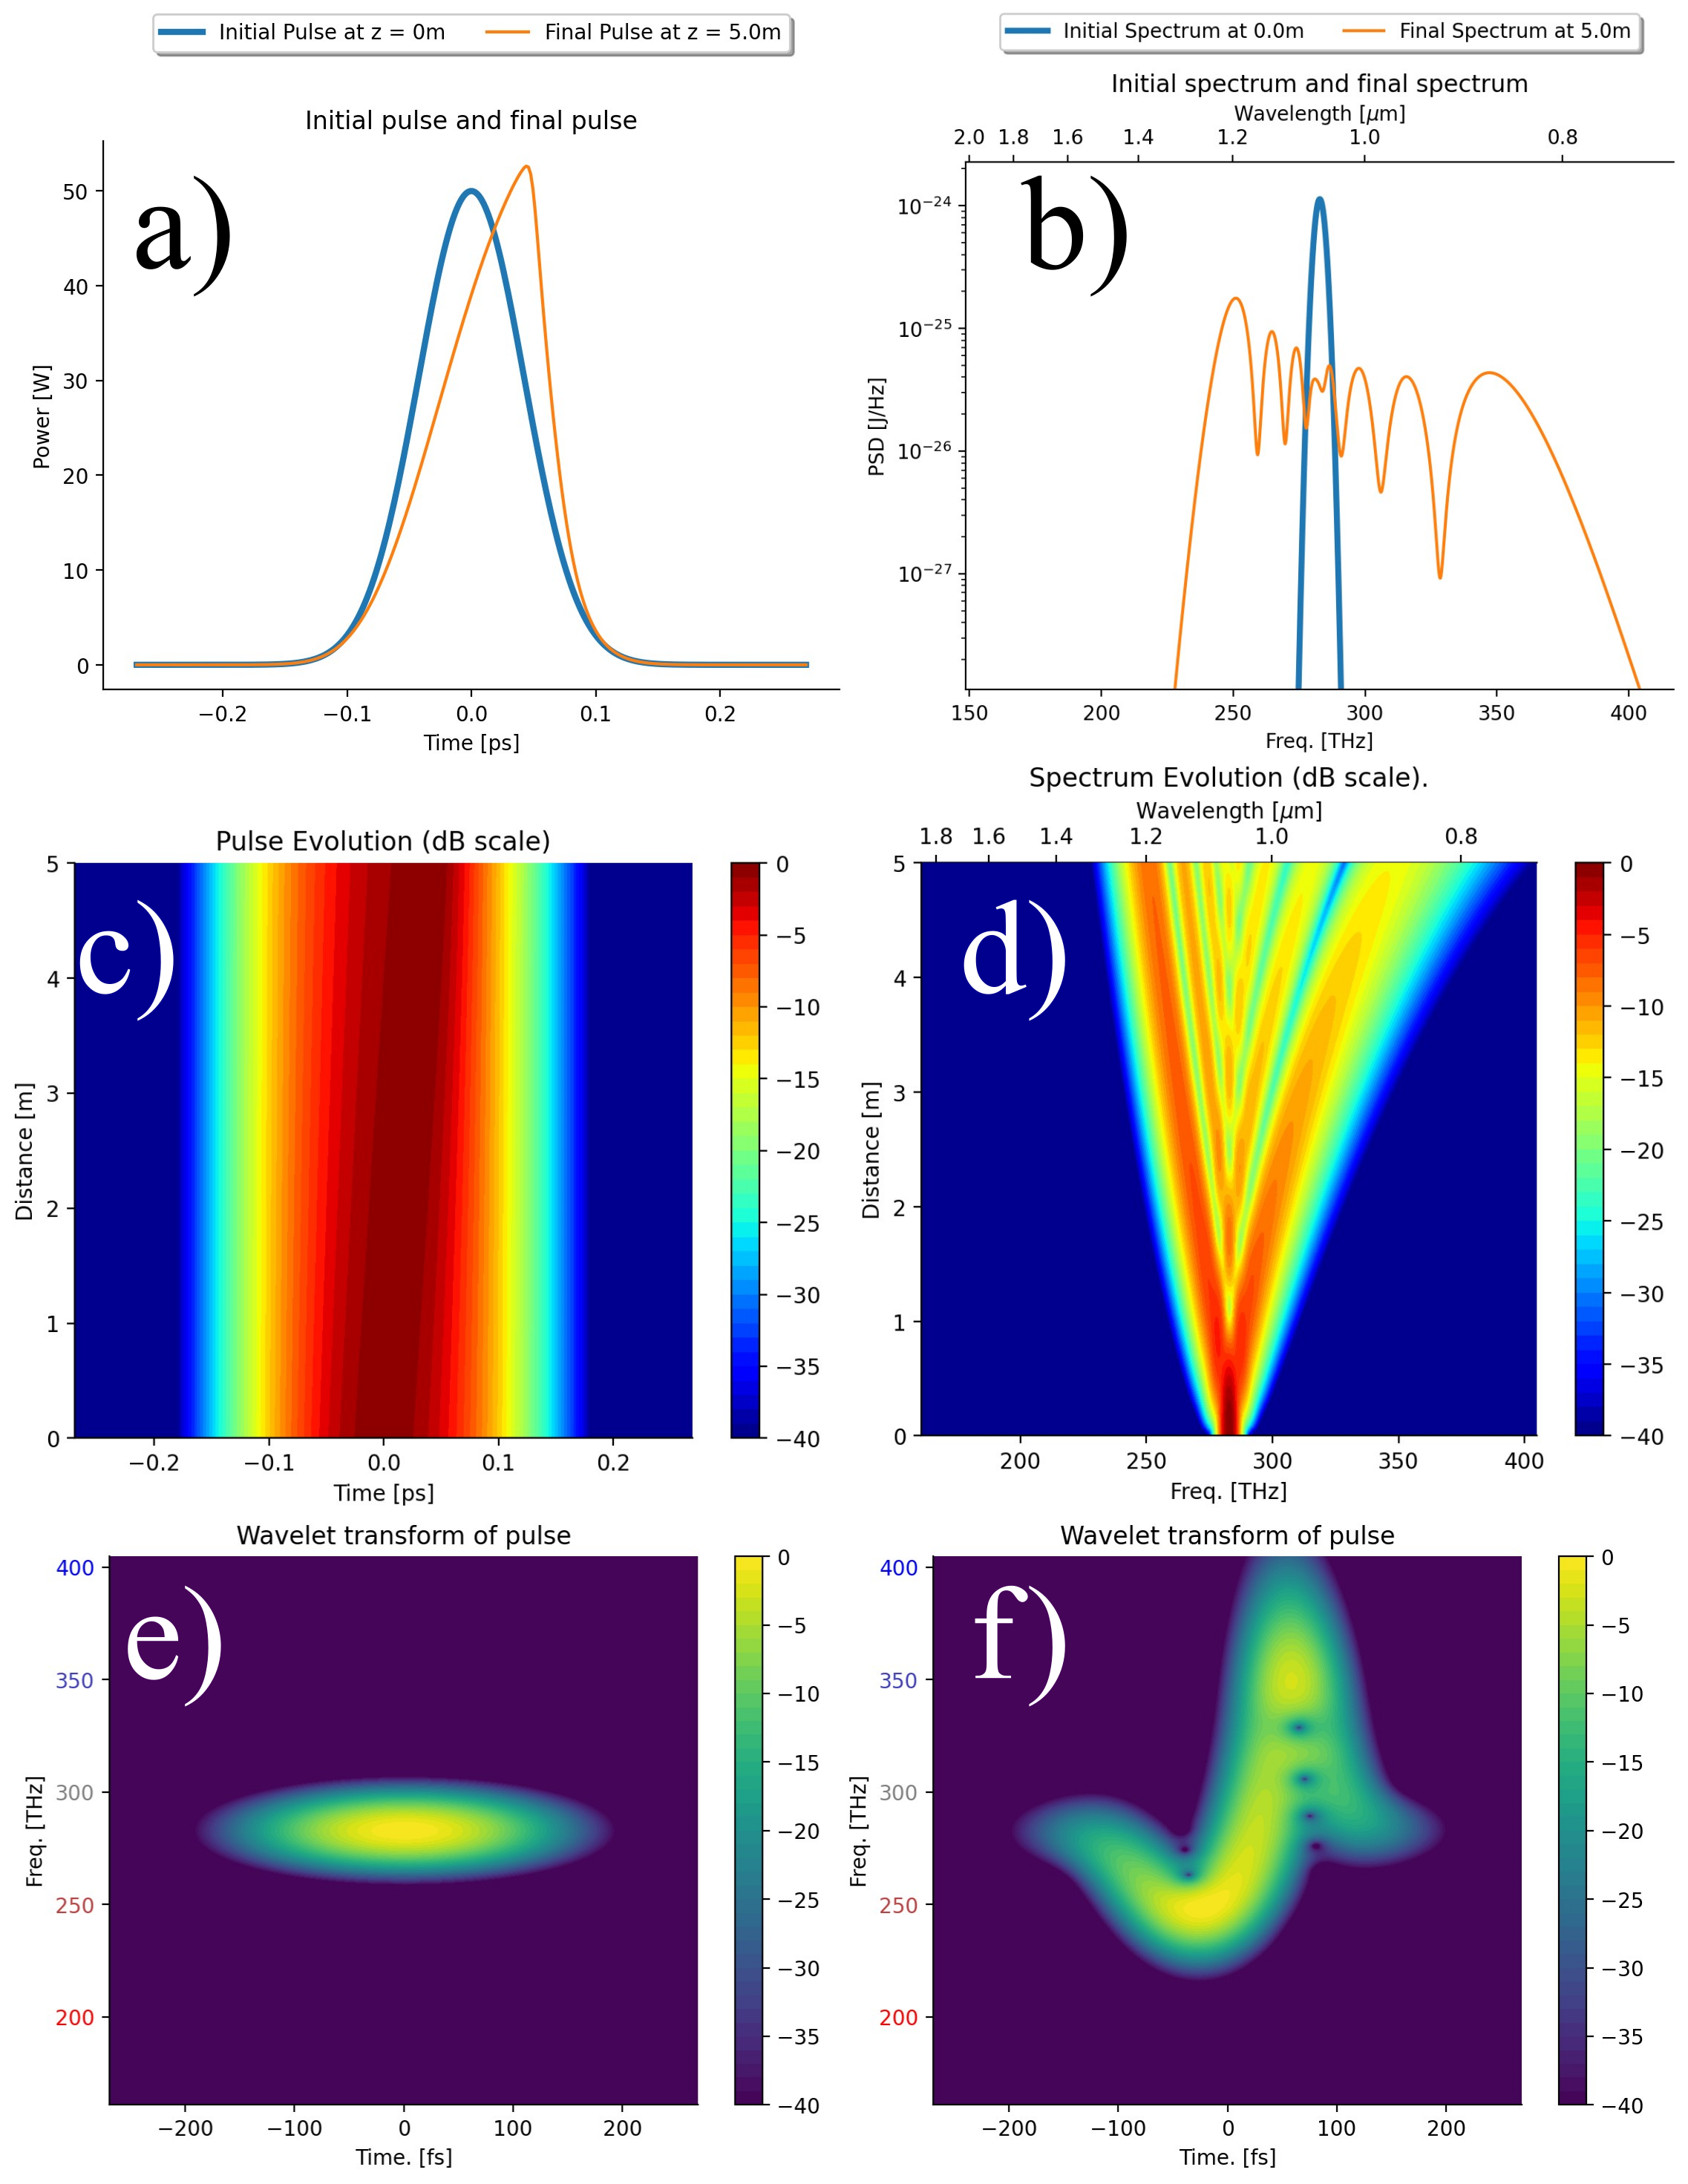
\includegraphics[width=1.0\linewidth]{figures/SPM_and_SS_combined.png}
    \caption{高斯脉冲在由等式~\ref{eq:SS}描述的非线性介质中传播的前后对比。 
    a) 在时域中,脉冲的功率包络在后端变得更陡,因为非线性效应导致脉冲峰值处的折射率较高并减速。 b) 频谱由于后端的陡降坡度向更高频率不对称展宽。 c) 时域中功率包络的演化。 d) 频谱逐渐向高频展宽。 e) 传播前的脉冲频谱图。 f) 传播后的脉冲频谱图。使用\href{https://colab.research.google.com/drive/1P41F4hO6Mv12RsEkpogYv5teQyFZ6iW0?usp=sharing}{这个交互notebook}中的数值模拟生成图形,读者可以尝试进行实验。}
    \label{fig:SS}
\end{figure}

\subsection{适用性}
由于SS的影响与 $\omega_0\approx 2\pi/200~\text{THz} = 2\pi/5$fs 成反比,且对于长脉冲 $\A|\A|^2$ 的时间导数较小,SS效应在脉宽低于100~fs时较为显著,在数百fs量级的脉宽时较为显著,而对于超过几ps的脉宽则可忽略不计。




    \chapter{Four Wave Mixing}
\label{ch:FWM}

The average power of a single frequency of light calculated from Eq.~\ref{eq:average_power} will be constant over time. If two frequencies are present, their interference will cause the average power to vary sinusoidally over time. Since $\gamma\neq0$ implies that the refractive index depends on power, the simultaneous presence of two frequencies of light in a nonlinear medium implies that the phase will be sinusoidally modulated. This effect generates new frequency components and is referred to as "Four Wave Mixing" (FWM).




\section{Electrical phase modulation}
To understand FWM, first consider a continuous wave laser signal launched into a commercially available phase modulator being driven by an sinusoidal electrical signal from a function generator. See Fig.~\ref{fig:PM} for a visualization and \href{https://youtu.be/j8It3to54AQ}{this video} for an experimental demonstration. The signal at the output is given by
\begin{align}
    \label{eq:phase_modulator}
    \E_{out}&=\E_{in}\exp\left(i\Phi\cos(\omega_dT), \right)
\end{align}
where $\Phi$ is the maximum phase shift imparted by the modulator and $\omega_d$ is the modulation frequency. See \href{https://www.desmos.com/calculator/vcreo1gs2q}{this interactive graph} for an illustration of the impact of this modulation on the real part of $\E_{out}$. Using the so-called "Jacobi-Anger Expansion"~\cite{NIST_JA_expansion}, the cosine function inside the complex exponential in Eq.~\ref{eq:phase_modulator} can be written as
\begin{align}
\label{eq:JA}
    \exp\left(i\Phi\cos(\omega_dT)\right) &= \sum_{n=-\infty}^{\infty}i^n J_n(\Phi) \exp\left(in\omega_dT\right),
\end{align}
where $J_n(\Phi)$ is the $n^{th}$ order Bessel function of the 1st kind. In short, Eq.~\ref{eq:JA} shows that sinusoidal phase modulation gives rise to new discrete frequency components spaced $\omega_d$ apart and whose relative powers depend on the modulation amplitude, $\Phi$. Note also that applying Eq.~\ref{eq:chirp_definition} to Eq.~\ref{eq:phase_modulator} shows that the sinusoidal modulation changes the instantaneous frequency over time by $\Phi\omega_d\sin(\omega_dT)$, further suggesting that phase modulation changes the color of the incident light.

\begin{figure}
    \centering
    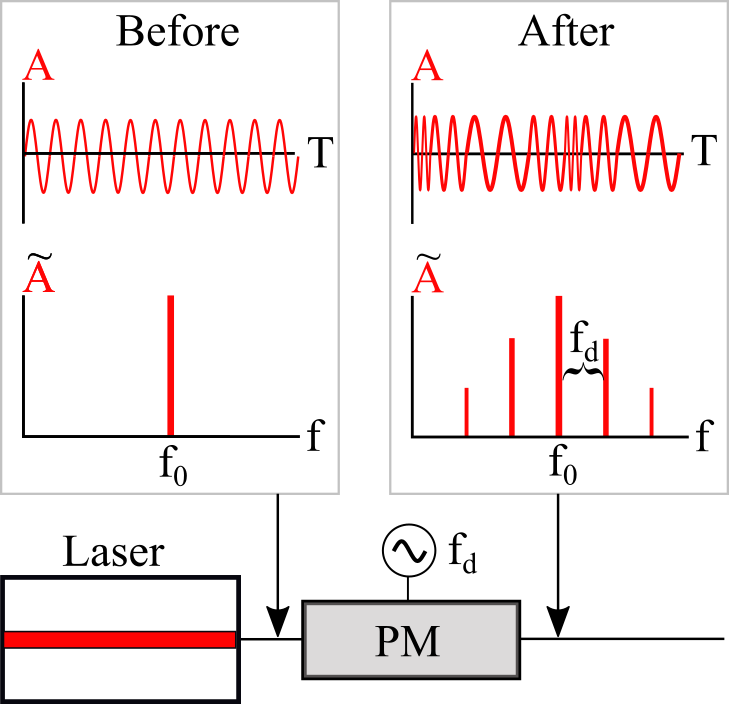
\includegraphics[width=1\linewidth]{figures/PhaseModulator.png}
    \caption{Illustration of the impact of electrical sinusoidal phase modulation of a continuous wave optical signal. Before entering the modulator, only a single laser frequency is present. After the modulator, the alternating advancement and delay of the optical phase in the time domain is equivalent to introducing new frequency components according to Eq.~\ref{eq:JA}.}
    \label{fig:PM}
\end{figure}

\section{Nonlinearity based phase modulation}
\label{sec:sidebands}
The following approach to modelling FWM is inspired by the one originally presented in~\cite{Boskovic_Original_Kerr_Effect}. Consider Eq.~\ref{eq:SPM_applied} and assume that the field, $\A(0,T)$ can be written as the sum of two continuous wave signals with average powers $P_a$ and $P_b$ and a frequency spacing of $\Delta\omega$ according to
\begin{align}
    \label{eq:FWM_input}
    \A(0,T)&= \sqrt{P_a}e^{-i\frac{\Delta\omega}{2}T}+\sqrt{P_b}e^{i\frac{\Delta\omega}{2}T}.
\end{align}
When the signal consists of two pulses with finite durations, the continuous wave assumption is an approximation, which is valid when $\omega_d$ is larger than the bandwidths of the pulses. The field at the end of the nonlinear medium is
\begin{align}
    \A(L,T) &= \A(0,T)\exp\left(i\gamma L [P_a+P_b+2\sqrt{P_aP_b}\cos(\omega_dT)] \right) \\ \nonumber
    &= \A(0,T)\exp\left(i\gamma L [P_a+P_b]\right)\exp\left(i2\gamma L\sqrt{P_aP_b}\cos(\omega_dT) \right)\\ \nonumber
    \A(L,T)Q^{-1}&= \A(0,T)\exp\left(i2\gamma L\sqrt{P_aP_b}\cos(\omega_dT) \right)\\ \nonumber
    \A(L,T)Q^{-1}&= \A(0,T)\exp\left(i\phi_{NL}\cos(\omega_dT) \right),
\end{align}
where the time-independent factor $Q=\exp(i\gamma L [P_a+P_b])$ is temporarily moved to the left hand side of the equality for convenience. Applying Eq.~\ref{eq:JA} yields
\begin{align}
    \A(L,T)Q^{-1}&= \A(0,T)\sum_{n=-\infty}^{\infty}i^nJ_n(\phi_{NL})e^{in\omega_dT} \\ \nonumber
    &=\left(\sqrt{P_a}e^{-i\frac{\Delta\omega}{2}T}+\sqrt{P_b}e^{i\frac{\Delta\omega}{2}T}\right)\sum_{n=-\infty}^{\infty}i^nJ_n(\phi_{NL})e^{in\omega_dT} \\ \nonumber
    &=\sqrt{P_a}\sum_{m=-\infty}^{\infty}i^mJ_m(\phi_{NL})e^{i\left(m-\frac{1}{2}\right)\omega_dT}+...\\ \nonumber & \quad\quad\quad\quad\quad\sqrt{P_b}\sum_{k=-\infty}^{\infty}i^kJ_k(\phi_{NL})e^{i\left(k+\frac{1}{2}\right)\omega_dT}.
\end{align}
Note that the infinite sum initially indexed by $n$ is split into two infinite sums indexed by $m$ and $k$ because the two complex exponentials in $\A(0,T)$ cause the frequency corresponding to $m=1$ in the first sum to be different from the one corresponding to $k=1$ in the second sum. To re-combine the two sums, use $m=k+1$ and obtain
\begin{align}
\label{eq:re_index}
    \A(L,T)Q^{-1}&=\sqrt{P_a}\sum_{k=-\infty}^{\infty}i^{k+1}J_{k+1}(\phi_{NL})e^{i\left(k+\frac{1}{2}\right)\omega_dT}+...\\ \nonumber & \quad\quad\quad\quad\quad\sqrt{P_b}\sum_{k=-\infty}^{\infty}i^kJ_k(\phi_{NL})e^{i\left(k+\frac{1}{2}\right)\omega_dT} \\ \nonumber
    &= \sum_{n=-\infty}^{\infty} i^n\left[i\sqrt{P_a}J_{n+1}\left(\phi_{NL}\right)+\sqrt{P_b}J_n\left(\phi_{NL}\right)\right]e^{i\omega_d\left(n+\frac{1}{2}\right)T}.
\end{align}
Finally, moving $Q$ to the right hand side of Eq.~\ref{eq:re_index} yields
\begin{align}
\label{eq:FWM_general}
    \A(L,T)&=\sum_{n=-\infty}^{\infty} i^n\left[i\sqrt{P_a}J_{n+1}\left(2\gamma L\sqrt{P_aP_b}\right)+\sqrt{P_b}J_n\left(2\gamma L\sqrt{P_aP_b}\right)\right]e^{i\omega_d\left(n+\frac{1}{2}\right)T+i\gamma L[P_a+P_b]}.
\end{align}
In Eq.~\ref{eq:FWM_general}, the frequency component for which $n=-1$ will be at $-\omega_d/2$, while the one for which $n=0$ will be at $+\omega_d/2$, corresponding to the original two frequencies in Eq.~\ref{eq:FWM_input}. The average power of the $n^{th}$ order sideband is
\begin{align}
\label{eq:sideband_power}
    |\A_n(L,T)|^2 &= P_aJ^2_{n+1}\left(2\gamma L \sqrt{P_aP_b}\right)+P_bJ^2_{n}\left(2\gamma L \sqrt{P_aP_b}\right).
\end{align}
See Fig.~\ref{fig:FWM} a) and b) for a numerical simulation of the sideband powers for different values of $2\gamma L \sqrt{P_aP_b}$. See Fig.~\ref{fig:FWM} c) for a comparison of the numerically calculated sideband powers and the ones predicted by Eq.~\ref{eq:sideband_power}. Assuming that $P_a\ll P_b$ and $2\gamma L\sqrt{P_aP_b}<\sqrt{1+n}$ with $n>0$ yields
\begin{align}
\label{eq:sideband_approx}
    |\A_n(L,T)|^2 &\approx P_b\frac{(\gamma^2 L^2P_aP_b)^{n}}{n!^2},
\end{align}
since
\begin{align}
\label{eq:Bessel_approx}
    J_n(x)&\approx \frac{1}{n!}\left(\frac{x}{2}\right)^n
\end{align}
for small arguments in the Bessel function. See Fig.~\ref{fig:FWM} d) for an illustration of the scaling behavior predicted by Eq.~\ref{eq:sideband_approx}. The fact that the power of higher order sidebands is more sensitive to changes in input power than lower order ones is useful for various all-optical signal processing techniques~\cite{my_thesis,BenoitPhD,YangLuPhD}. See \href{https://youtu.be/0SXPvO89jto}{this tutorial video} for a different approach to modelling FWM that takes dispersion into account. See \href{https://youtu.be/gsa9hrCbnqI}{this video} for an experimental demonstration of FWM. 
\begin{figure}
    \centering
    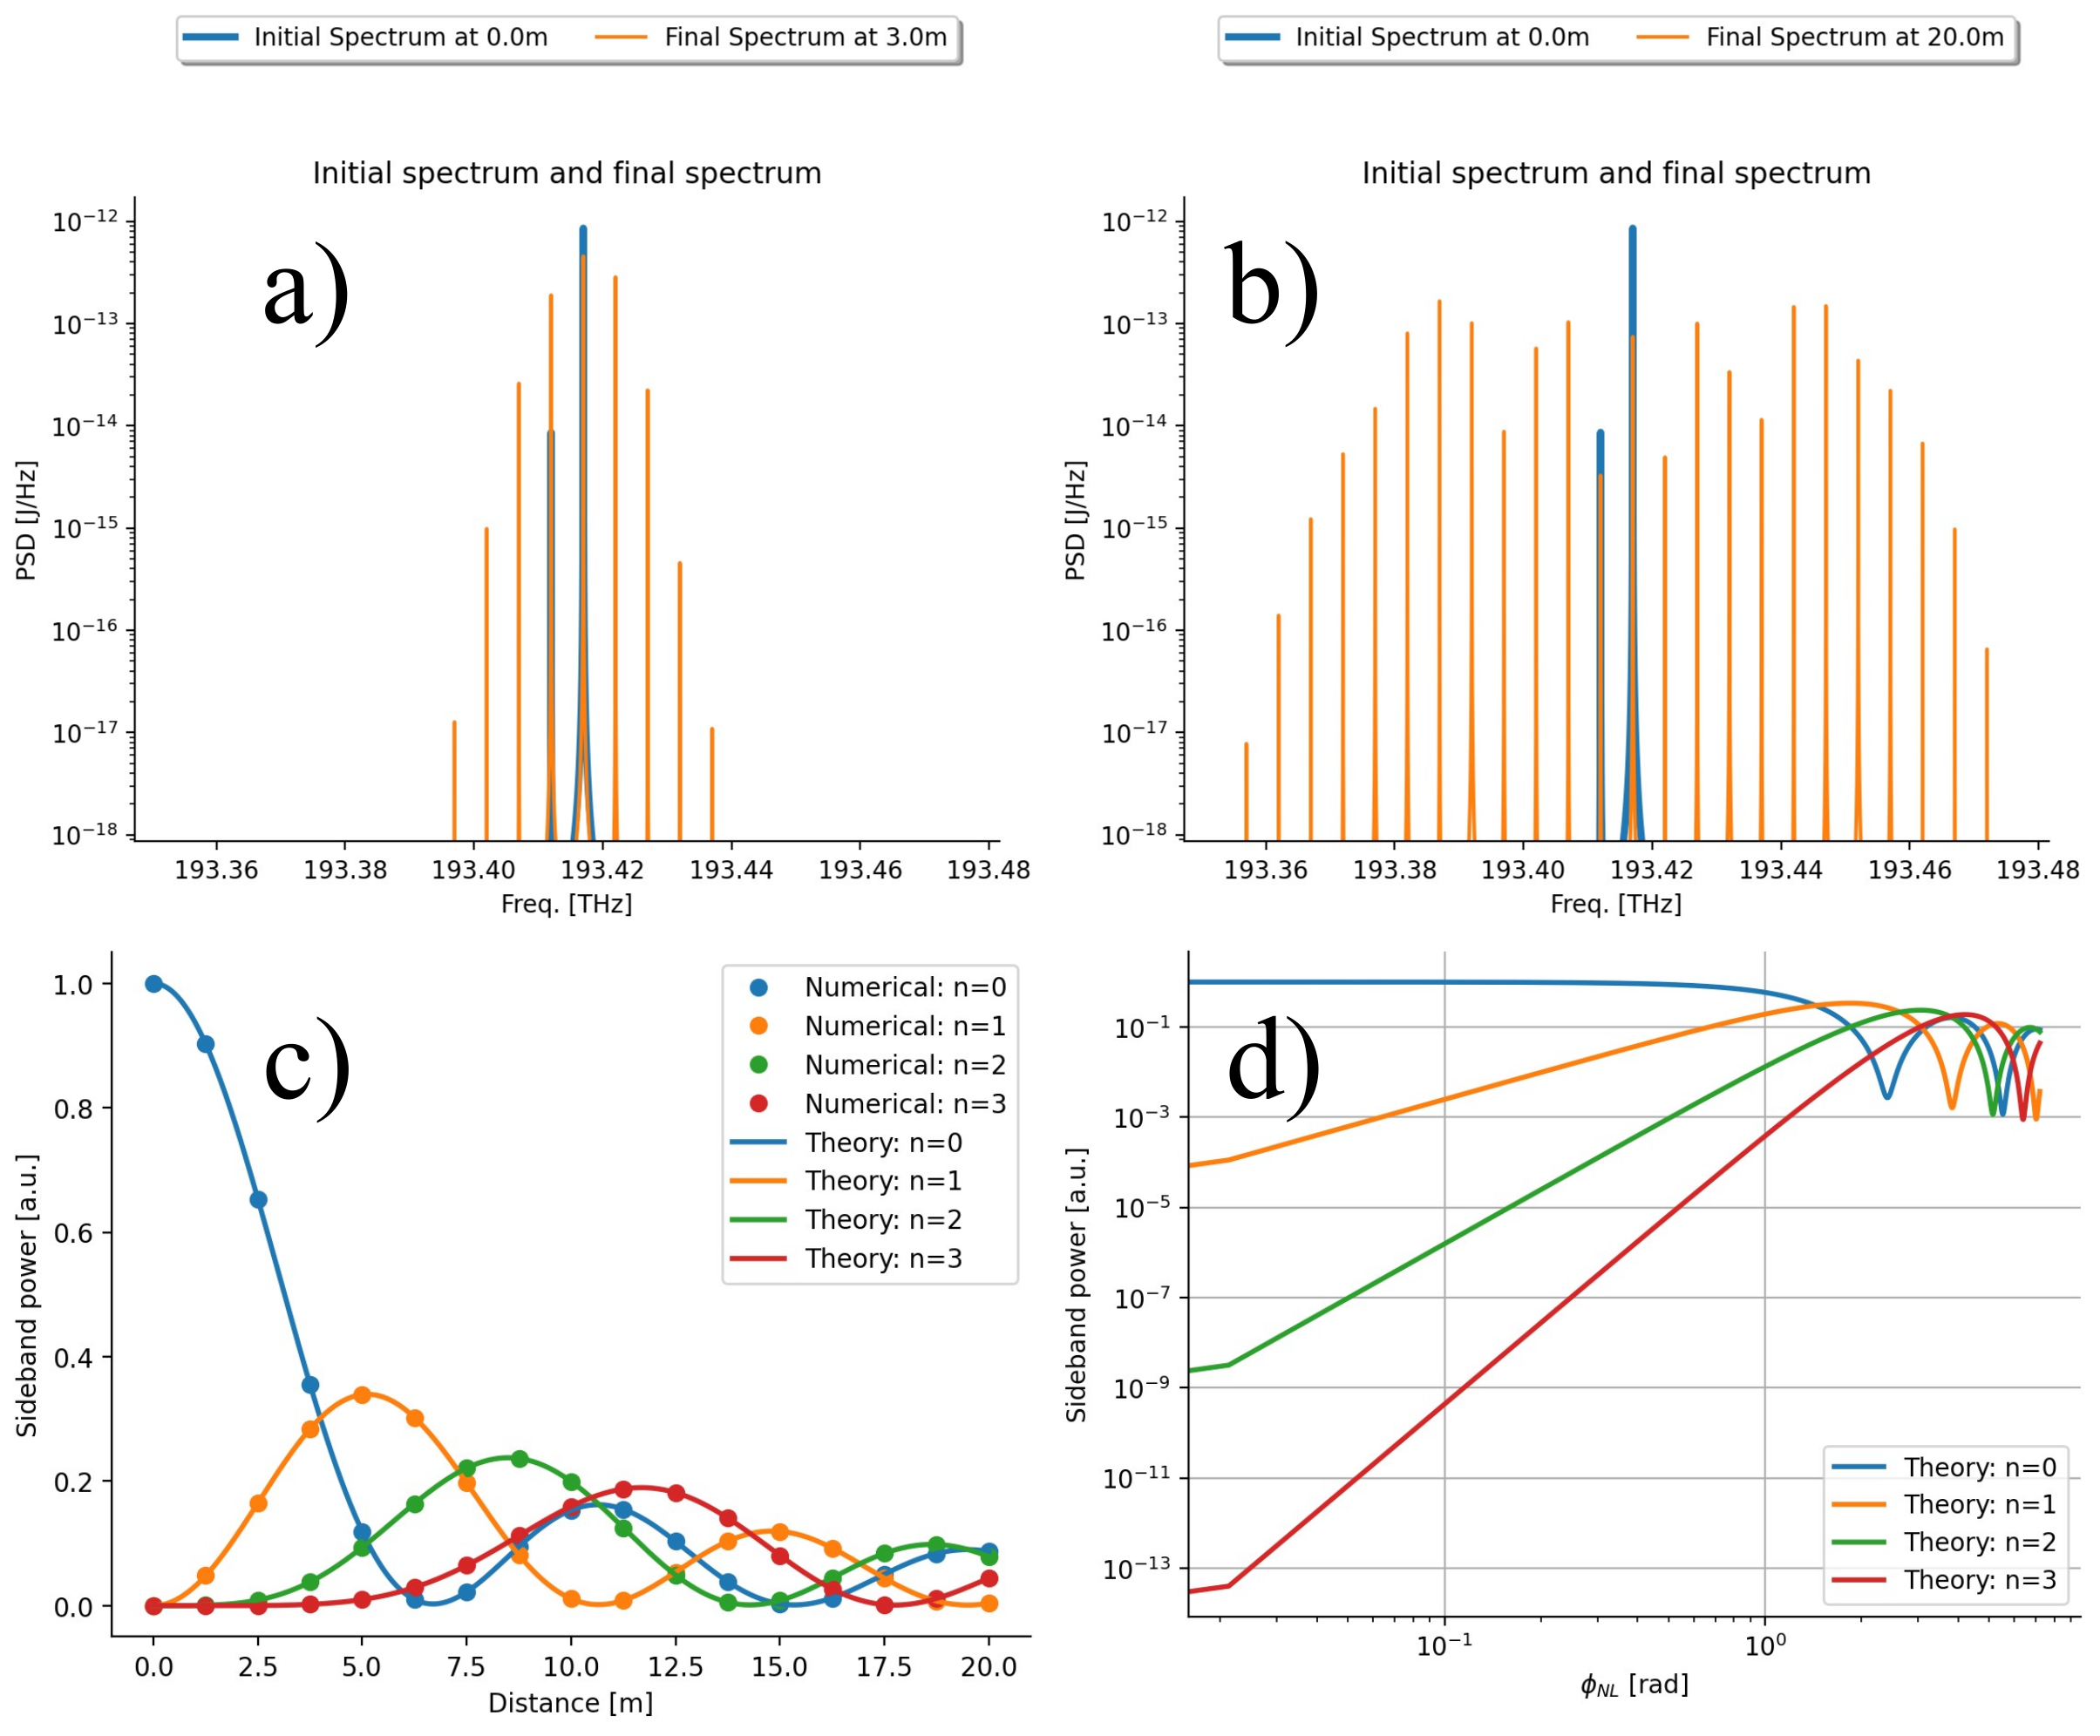
\includegraphics[width=1.0\linewidth]{figures/FWM_combined.png}
    \caption{a) Numerically calculated initial and final spectrum when two frequencies with $P_b=100P_a$ spaced 5~GHz apart  propagate through a medium where $\phi_{NL}=2\gamma L\sqrt{P_aP_b}=1.08$~rad. Note the transfer of power from the most intense frequency into neighbouring sidebands and the rapid decrease in power for increasing sideband orders as predicted by Eq.~\ref{eq:sideband_approx}. b) Same as a) but for $\phi_{NL}=2\gamma L\sqrt{P_aP_b}=7.2$~rad. c) Comparison of sideband power normalized to $P_b$ according to numerical simulations and Eq.~\ref{eq:sideband_power}. d) Similar to c) but plotted on a double-log scale versus $\phi_{NL}$ to demonstrate the scaling behavior predicted by Eq.~\ref{eq:sideband_approx}. Figures generated using \href{https://colab.research.google.com/drive/1l054EDg-50aK5GORN_md4_-tlFy4jwC5?usp=sharing}{this interactive notebook}, which the reader is encouraged to experiment with.   }
    \label{fig:FWM}
\end{figure} 

\section{Cross Phase Modulation (XPM)}
\label{Sec:XPM}
In Chapter~\ref{ch:SPM}, it was shown that the phase of a single-frequency optical field in a nonlinear medium increases linearly with the average power of that field. When two frequencies are present, the phase of one frequency component as a function of its own average power and the average power of the other can be calculated from Eq.~\ref{eq:FWM_general}. Choosing the $n=0$ component yields
\begin{align}
    \phi_0 &= \frac{\omega_d}{2}T+\gamma L [P_a+P_b]+\theta_0,
\end{align}
where
\begin{align}
\label{eq:theta}
    \theta_0 &= arg\left( i\sqrt{P_a}J_{1}\left(2\gamma L\sqrt{P_aP_b}\right)+\sqrt{P_b}J_0\left(2\gamma L\sqrt{P_aP_b}\right) \right) \\ \nonumber
    &= \arctan\left(\frac{\sqrt{P_a}J_{1}\left(2\gamma L\sqrt{P_aP_b}\right)}{\sqrt{P_b}J_0\left(2\gamma L\sqrt{P_aP_b}\right) } \right).
\end{align}
Using Eq~\ref{eq:Bessel_approx} allows Eq.~\ref{eq:theta} to be written as
\begin{align}
    \theta_0 &\approx\arctan\left(\frac{\sqrt{P_a}\gamma L\sqrt{P_aP_b}}{\sqrt{P_b} } \right) \\ \nonumber
    &\approx\arctan\left(\gamma LP_a\right) \\ \nonumber
    &\approx \gamma LP_a.
\end{align}
Thus, the phase of the $n=0$ frequency component is
\begin{align}
    \label{eq:XPM}
    \phi_0 &\approx \frac{\omega_d}{2}T+\gamma L [P_a+P_b]+\gamma LP_a \\ \nonumber
    &=\frac{\omega_d}{2}T+\gamma L [2P_a+P_b].
\end{align}
Note that $n=0$ is the frequency at $+\omega_d/2$, which initially had the average power $P_b$. Therefore, the term in Eq.~\ref{eq:XPM} containing $P_b$ corresponds to the impact of SPM, while the term containing $P_a$ corresponds to so-called "Cross Phase Modulation" (XPM). Interestingly, Eq.~\ref{eq:XPM} shows that XPM is "twice as strong" as SPM as demonstrated numerically in Fig.~\ref{fig:XPM}. See \href{https://youtu.be/aDXd13zLPC4}{this video tutorial} for an alternative derivation starting from Maxwell's Equations of the impact of XPM. See \href{https://www.desmos.com/calculator/vstlwgtlyb}{this interactive graph} for an illustration of the relative impact of SPM and XPM on two waves with different frequencies.

\begin{figure}
    \centering
    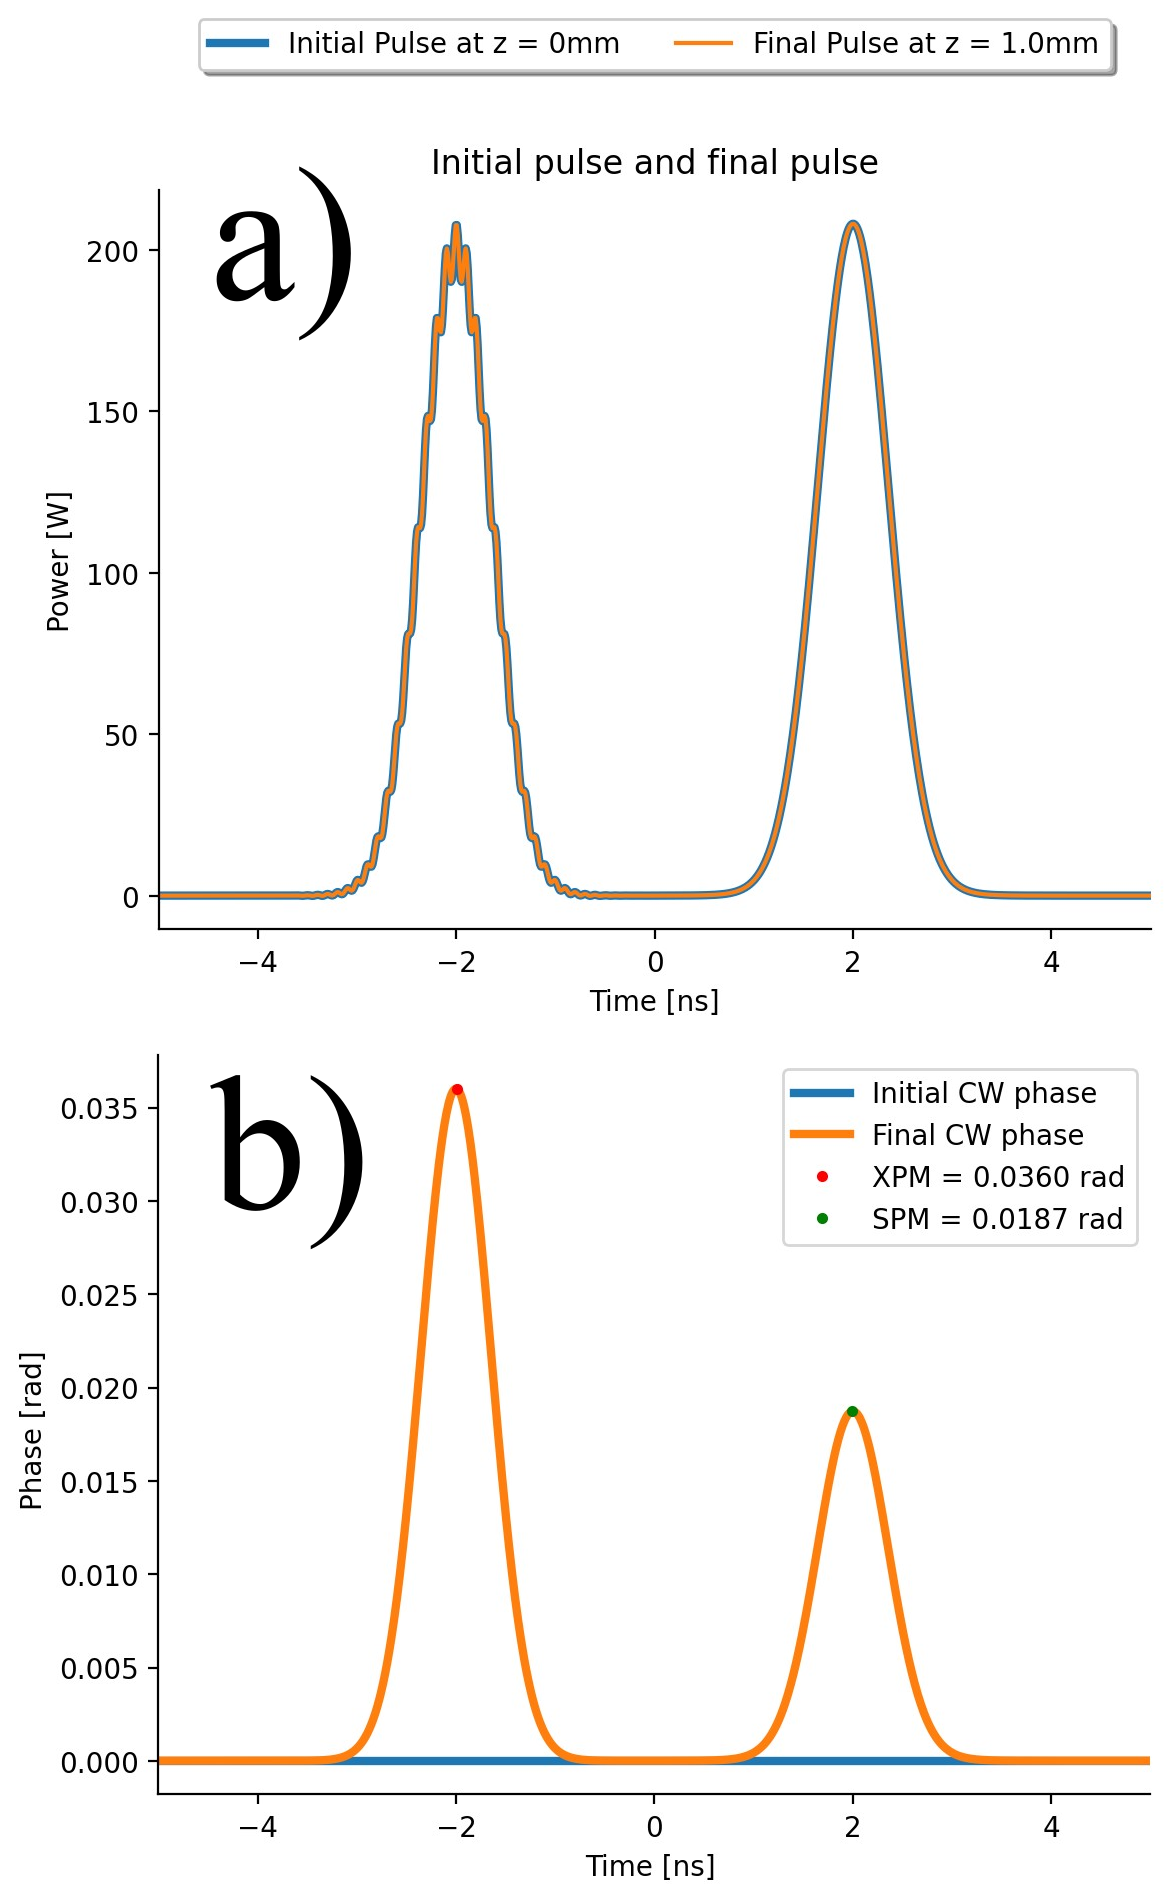
\includegraphics[width=0.8\linewidth]{figures/XPM_combined.png}
    \caption{Illustration of the disparate impacts of SPM and XPM on the phase of an optical signal. a) Time domain representation of a low power CW signal overlapped with two identical, high power Gaussian pulses that only differ by their carrier frequencies. The carrier frequency of the pulse on the left is 10~GHz below the carrier frequency of the CW light. b) After simulating the propagation through a nonlinear medium, the CW light obtains approximately twice the phase shift from XPM as from SPM as predicted by Eq.~\ref{eq:XPM}. The ratio of $0.0360/0.0187\approx 1.925\neq2$ is attributed to the approximations involved in Eq.~\ref{eq:XPM} and to the finite time resolution of the simulation. Figures generated using \href{https://colab.research.google.com/drive/1aIRradfOZGN7JYUhbtYJdVzJwAZoYoUe?usp=sharing}{this interactive notebook}, which the reader is encouraged to experiment with.}
    \label{fig:XPM}
\end{figure}






\section{Phase matching}
\label{sec:Phase_matching}
The derivation presented in Section~\ref{sec:sidebands} assumes negligible dispersion, which is the case for a small $\omega_d$ value and a carrier frequency close to the zero dispersion frequency explained in Subsection~\ref{subsec:ZDF}. The impact of dispersion on FWM is explained in \href{https://youtu.be/0SXPvO89jto}{this video tutorial}. It turns out that FWM is weak for positive values of $\betag_2$ and is most significant when
\begin{align}
\label{eq:phase_matching}
0&=\betag_2\omega_d^2+\gamma(P_a+P_b)    \\ \nonumber
\betag_2&=-\gamma(P_a+P_b)/\omega_d^2<0,    
\end{align}
assuming that $\omega_d$ is small enough for $\betag_2$ to be the only relevant term in Eq.~\ref{eq:beta_approx}. The reason is that FWM as a process involves the \emph{coherent} transfer of power from one set of electromagnetic waves into oscillating changes in the refractive index of the nonlinear medium and then into another set of electromagnetic frequencies. In short, the nonlinearity ensures that the incident electromagnetic waves will cause the tiny dipoles constituting the medium to oscillate at new temporal frequencies. If the corresponding spatial frequency of one of these temporal oscillations in the dipoles is the same as the spatial frequency of another electromagnetic wave, its power will increase with distance via constructive interference as explained in \href{https://youtu.be/bha8SzWzRc4}{this video tutorial}. The requirement in Eq.~\ref{eq:phase_matching} arises because the difference in spatial frequencies of the incident waves and the new wave should be small and because the increase in the refractive index due to the power of the initial fields makes the spatial frequencies larger than they normally would be. Thus, a negative values of $\betag_2$ is needed to compensate. This effect, where the spatial frequencies caused by the regular refractive index of the medium balance changes in the spatial frequencies due field power via nonlinearity, is referred to as "phase matching". The phase matching condition in Eq.~\ref{eq:phase_matching} is relevant for the special case of FWM and similar expressions can be derived for other nonlinear effects beyond the scope of this primer, such as \href{https://www.youtube.com/watch?v=UpuN0dS23Nw}{Second-Harmonic generation} , \href{https://youtu.be/bha8SzWzRc4}{Third-Harmonic generation} and \href{https://www.creol.ucf.edu/mir/wp-content/uploads/sites/7/2023/07/L22_-Stimulated-Brillouin-scattering.pdf}{Stimulated Brillouin Scattering}.  

\subsection{Modulation Instability}
As a consequence of FWM, a signal with a carrier frequency where $\betag_2<0$ for a particular nonlinear medium will get noisier as it propagates forward. The reason is that the interference between the carrier and tiny, ubiquitous fluctuations in the electromagnetic field will cause FWM to transfer optical power away from the carrier and into adjacent frequencies as explained \href{https://prefetch.eu/know/concept/modulational-instability/}{here} and illustrated in Fig.~\ref{fig:MI}. The process of particular noise frequencies being preferentially amplified due to phase matching is referred to as "Modulation Instability" (MI). See \href{https://youtu.be/VtaoPd0Fwj8}{this video tutorial} for further details on MI. 

\begin{figure}
    \centering
    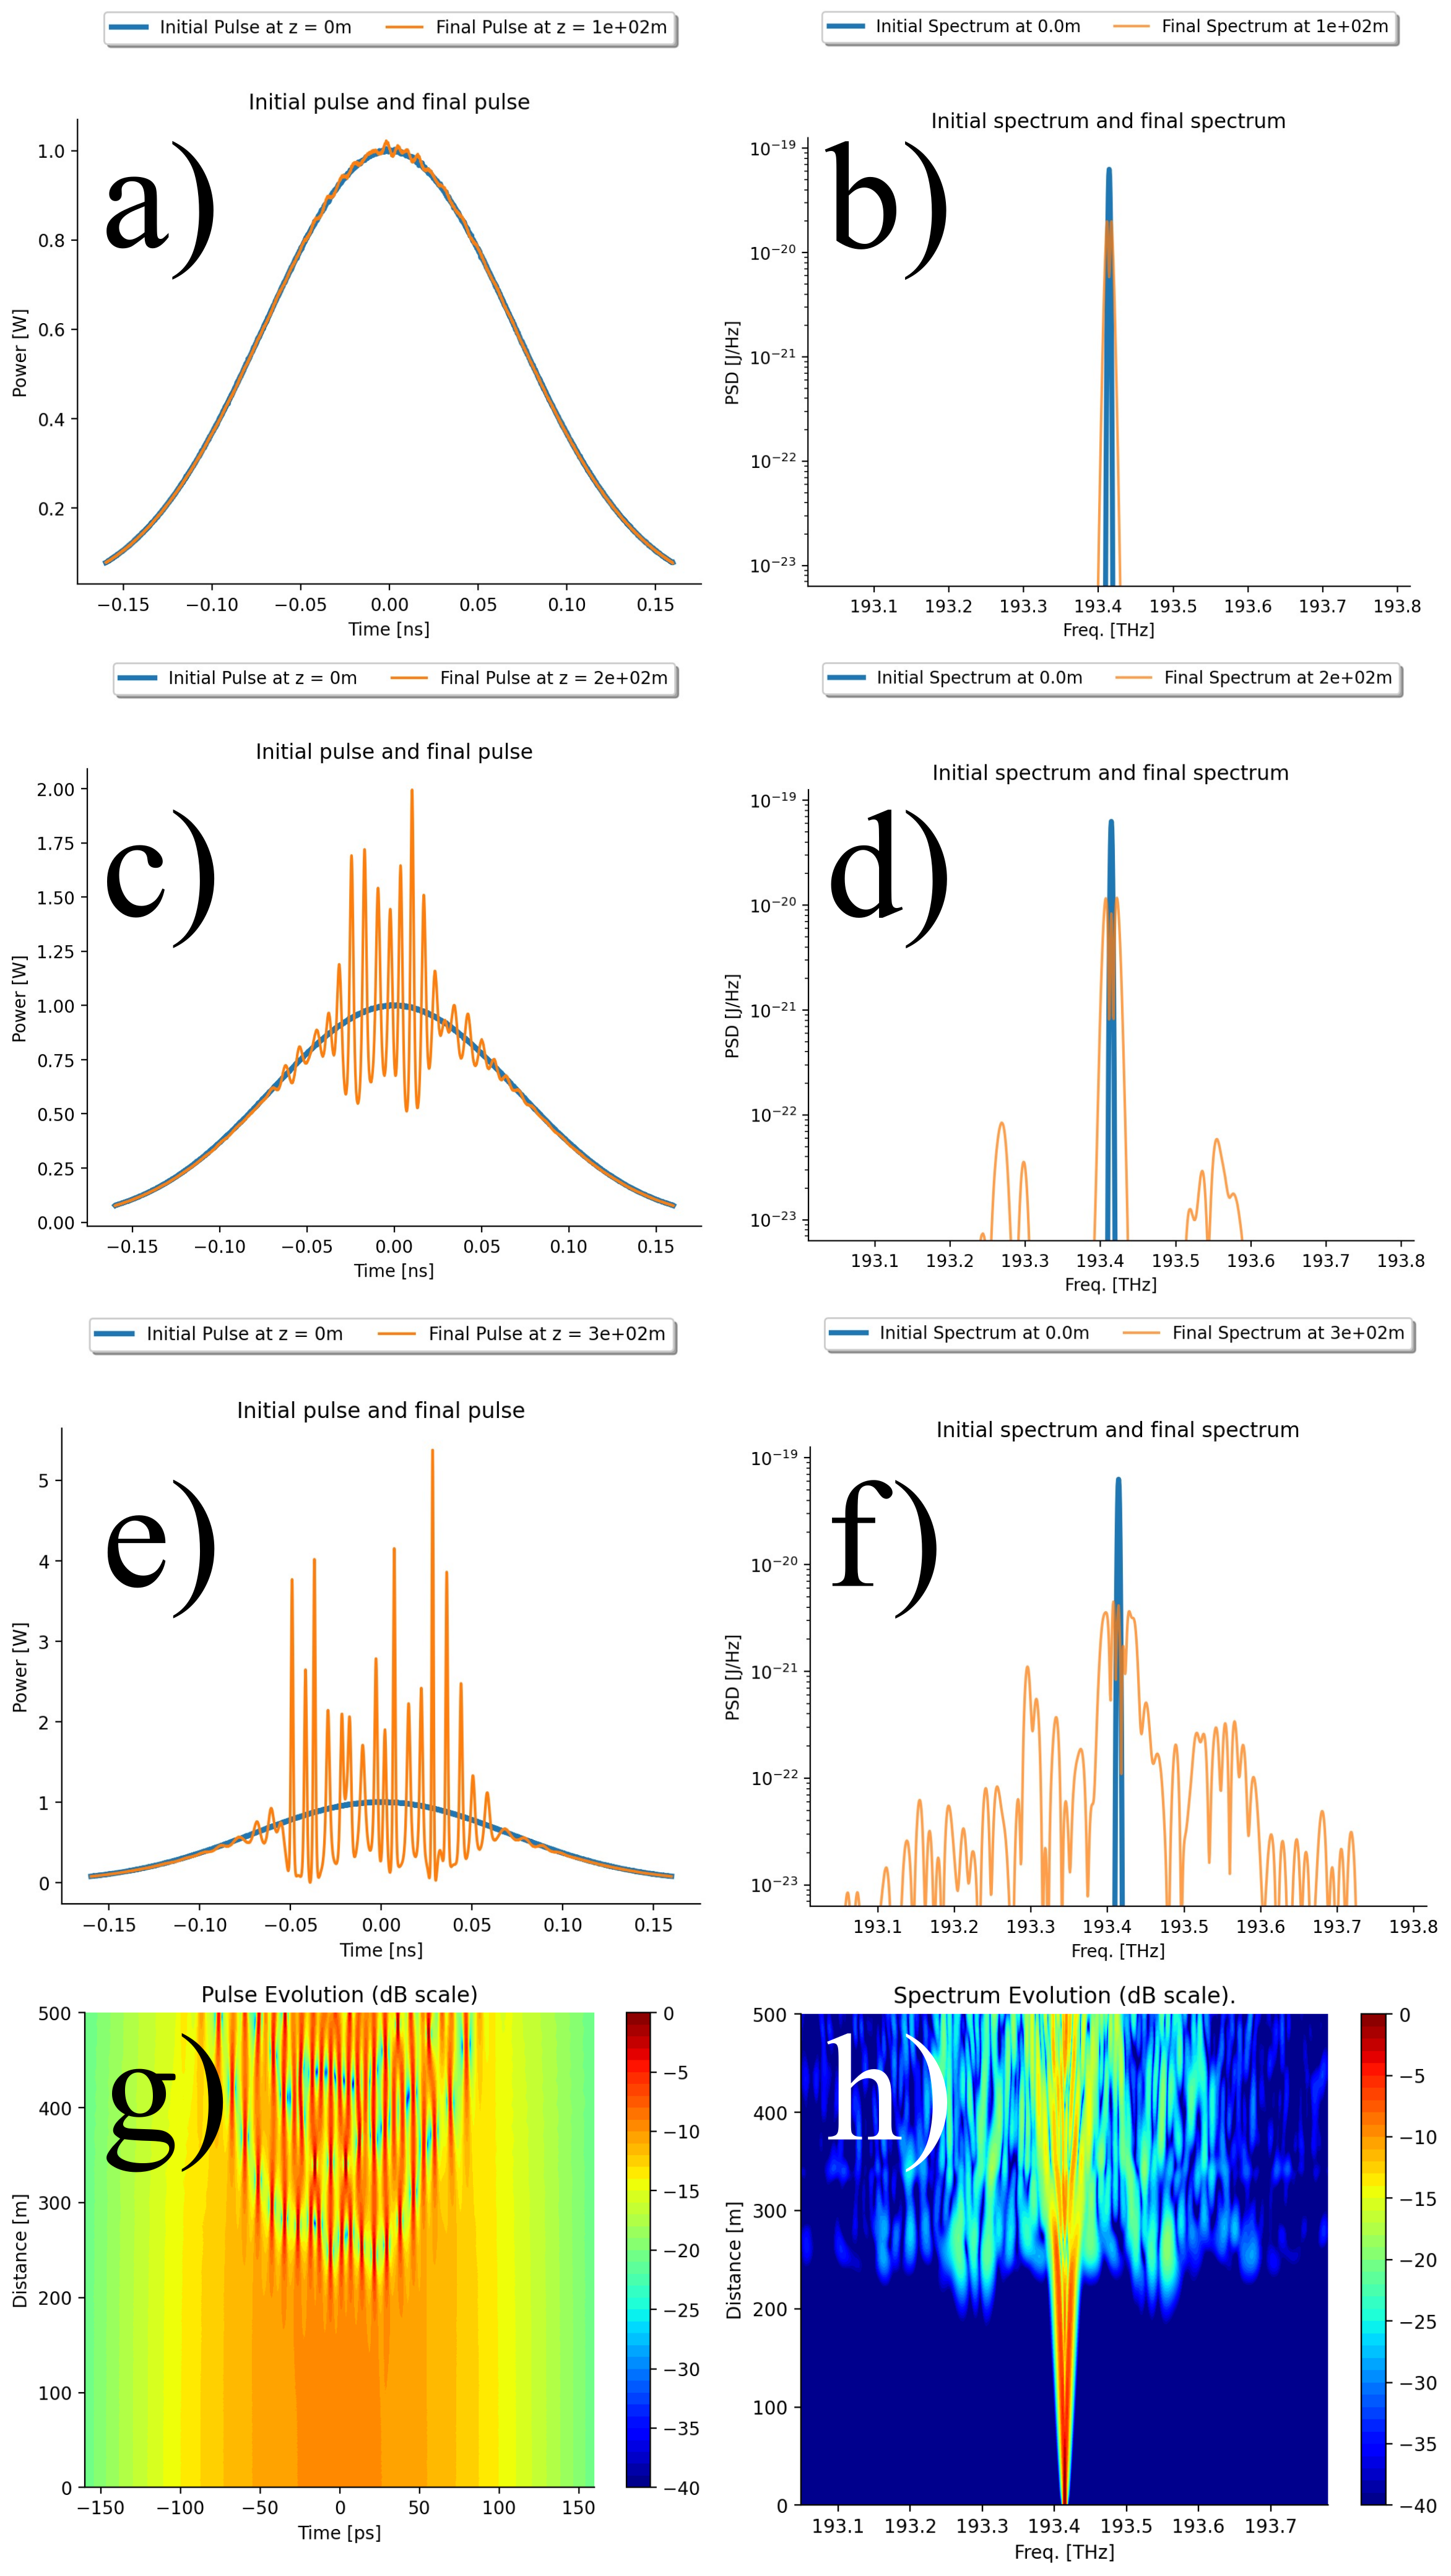
\includegraphics[width=0.75\linewidth]{figures/MI_combined.png}
    \caption{a) Initial and final time domain power of a signal consisting of a Gaussian pulse and random noise with an amplitude 1.000 times smaller than that of the Gaussian propagated through 100m of a nonlinear medium with $\betag_2<0$. b) Same as a) but showing the spectrum. c-d) Same as a-b) but for a distance of 200m. e-f) Same as a-b) but for a distance of 300m. g) full temporal evolution for 500m. h) Same as g) but for the spectrum. Figures generated using \href{https://colab.research.google.com/drive/1p2aQZ4zPPAIMplVxvlezdmpQt_j-rsY7?usp=sharing}{this interactive notebook}, which the reader is encouraged to experiment with.}
    \label{fig:MI}
\end{figure}




    \chapter{拉曼效应}
\label{ch:Raman}

当暴露在振荡电磁场中时,介质中的电子由于质量较小,几乎会立即做出反应。而这些电子绕其运行的原子核由于质量相对较大,反应速度要慢得多。因此,影响某一光纤段脉冲特定瞬间的非线性相移取决于两点: 该瞬间脉冲的光功率和过去影响该位置的光功率。材料晶格中原子核的延时机械振动对电磁场的非线性影响被称为 “拉曼效应”~\cite{Raman_original}。 


\section{拉曼响应函数}
在数学上,拉曼效应对光脉冲的影响可以用以下公式描述
\begin{align}
\label{eq:raman}
 \partial_z \A = i\gamma\left( 
\A \int_{0}^{\infty} R(T_{delay})|\A(z,T-T_{delay})|^2 dT_{delay} \right),
\end{align}
在忽略损耗、色散和自陡的情况下,它等价于公式 ~\ref{eq:GNLSE}。函数 $R(T_{delay})$ 是总响应函数,表示过去不同时间的功率对给定瞬间影响脉冲的非线性相移的贡献程度。它可以通过三角函数写成电子响应的瞬时贡献与晶格振动引起的延迟拉曼响应之和,即
\begin{align}
    \label{eq:response}
    R(T_{delay})&= (1-f_R)\delta(T_{delay})+f_Rh_R(T_{delay}),
\end{align}
其中,$0\leq f_R\leq 1$ 是一个标量,决定了两个贡献的相对大小。拉曼响应函数的确切函数形式 $h_R(T_{delay})$ 取决于材料,但通常类似于一个乘以阻尼项的正弦函数,并且必须满足 $\int_{-\infty}^{\infty}h_R(T_{delay}) dT_{delay}=1$,因为它本质上是 “权衡 ”过去不同时间的功率对当前非线性相移的贡献程度。 此外,必须要求 $h_R(T_{delay})=0$ for $T_{delay}\leq0$ 以防止该表达式违反因果关系,让 \emph{future} 功率影响当前的非线性相移。请参阅 \href{https://www.desmos.com/calculator/bdg6icprch}{此交互图},了解过去的功率对拉曼效应引起的相移的影响。
直观地说,函数 $h_R(T_{delay})$就像描述音叉、钢琴键或吉他弦突然被敲击后声波振幅的函数一样,是一种逐渐 “回落 ”的振荡。继续类比,如果把 $|\A(z,T-T_{delay})|^2$ 看作是在不同时间具有不同强度的瞬时击打的大集合,那么当前的振荡取决于过去的所有振荡就说得通了。 
将公式 ~\ref{eq:response}代入公式 ~\ref{eq:raman},并对三角函数进行积分求得
\begin{align}
    \label{eq:raman_split}
    \partial_z \A = i\gamma\A\left( 
(1-f_R)|\A(z,T)|^2+f_R \int_{0}^{\infty} h_R(T_{delay})|\A(z,T-T_{delay})|^2 dT_{delay} \right).
\end{align}
请注意,如果脉冲功率的变化与响应函数的持续时间相比非常缓慢,则可以近似地计算 $h_R(T_{delay})\approx \delta(T_{delay})$(或者,等价地计算 $|\A(z,T-T_{delay})|^2\approx|\A(z,T)|^2$),在这种情况下,公式~\ref{eq:SPM}就恢复了。换句话说,只有当脉冲持续时间接近分子晶格自然振荡的持续时间时,拉曼效应才会明显!假设脉冲持续时间明显长于 $h_R(T_{delay})$的持续时间,因此不同时间延迟下的功率可以通过将当前功率及其梯度线性外推到过去来找到,那么公式~\ref{eq:raman_split}中的积分可以写为 
\begin{align}
\label{eq:raman_approx}
    f_R \int_{0}^{\infty} h_R(T_{delay})|\A(z,T-T_{delay})|^2 dT_{delay} &\approx\\ \nonumber \quad\quad\quad f_R \int_{0}^{\infty} h_R(T_{delay})\left[ 
  |\A(z,T)|^2-T_{delay}\partial_T|\A(z,T)|^2 \right] dT_{delay} &=\\ \nonumber \quad\quad\quad  |\A(z,T)|^2f_R- \partial_T|\A(z,T)|^2 f_R\int_{0}^{\infty} T_{delay} h_R(T_{delay}) 
   dT_{delay}&=\\ \nonumber \quad\quad\quad  |\A(z,T)|^2f_R- \partial_T|\A(z,T)|^2 T_R &,
\end{align}
其中 $T_R$ 是拉曼响应函数的平均持续时间,用 $f_R$ 缩放。将公式~\ref{eq:raman_approx}的结果代入公式~\ref{eq:raman_split}可得
\begin{align}
    \label{eq:raman_approx_applied}
\partial_z \A = i\gamma\A\left( 
|\A(z,T)|^2-T_R \partial_T|\A(z,T)|^2\right),
\end{align}
其中包含与电流功率成比例的 “常规 ”SPM 项,以及取决于功率时间导数的附加项。对于二氧化硅,$T_R/approx 3$~fs,因此公式 ~\ref{eq:raman_approx_applied}将对超过约 600~fs 的脉冲有效。公式 ~\ref{eq:raman_approx}中应用的近似值可以扩展到包括 $|\A(z,T)|^2$ 的二阶导数,以提高精确度。从公式 ~\ref{eq:SPM_example} 和 Fig.~\ref{fig:chirp_profiles} 中回想一下,“常数 ”SPM 项会导致瞬时频率大幅下降,而此时功率的 \emph{derivative} 值非常正(原文如此)。根据同样的逻辑,公式 ~\ref{eq:raman_approx_applied}中的拉曼项会导致 “导数的导数 ”为负的瞬时频率大幅下降。换句话说,拉曼效应会在脉冲峰值处产生红移,而在其他地方不会产生等效的大蓝移,从而使整个脉冲 “更红”!从物理学角度来看,红移的产生是因为入射光子会激发介质晶格的机械振动,从而损失部分能量。
\subsection{$h_R(T_{delay})$的表达式}
假设分子振动以单一频率为主,二氧化硅中拉曼效应的近似表达式为 
\begin{align}
\label{eq:raman_basic}
    h_R^{basic}(T_{delay})&= \left(\frac{1}{\tau_1^{2}}+\frac{1}{\tau_2^{2}} \right)\tau_1\exp\left(-\frac{T_{delay}}{\tau_2}\right)\sin\left(\frac{T_{delay}}{\tau_1}\right),
\end{align}
其中 $f_R=0.18$,$\tau_1=12.2$~fs,$\tau_2=32$~fs。为了尊重因果关系,所有列出的 $h_R(T_{delay})$表达式都假定 $T_{delay}\leq0$ 为零。在数学上,这可以通过乘以 Heaviside 阶跃函数来确保。对于二氧化硅的振动行为,比公式 ~\ref{eq:raman_basic} 更精确的近似值是  
\begin{align}
\label{eq:raman_new}
    h_R^{better}(T_{delay})&= (1-f_b) h_R^{basic}(T_{delay})+f_b\frac{2\tau_b-T_{delay}}{\tau_b^2}\exp\left(-\frac{T_{delay}}{\tau_b}\right),
\end{align}
其中,$f_R=0.245$,$f_b=0.21$,$\tau_b=96$~fs。二氧化硅拉曼响应的精确表达式为
\begin{align}
\label{eq:Raman_exact}
    h_R^{exact}(T_{delay})&=c^{-1}_{norm}\sum_{n=0}^{12}C_n\exp\left(- g_nT_{delay}-0.25G_n^2T^2_{delay}  \right)\sin\left(2\pi \nu_nT_{delay} \right),
\end{align}
其中,$f_R=0.18$,参数$C_n$、$g_n$、$G_n$和$\nu_n$列于表 ~\ref{tab:raman_coeffs},$c_{norm}=3.75225$~ps,因此$\int_0^\infty h_R^{exact}(T_{delay}) dT_{delay}=1$。图 ~\ref{fig:raman_combined}展示了这三种二氧化硅拉曼响应模型的可视化及其对同一光脉冲的影响。图 ~\ref{fig:raman_combined}~b) 中绘制了 $h_R(T_{delay})$ 不同表达式的傅立叶变换虚部。从物理角度看,这些光谱意味着拉曼效应允许特定光学频率从其上方 13~THz 的频率 “窃取 ”功率,并迫使其向下方 13~THz 的频率 “捐赠 ”功率。由于与章节 ~\ref{sec:KK_relations}中所述的原因类似,光谱的实部(未显示)与拉曼效应引起的折射率变化有关,因此可以确定其引起的时间延迟。根据图 ~\ref{fig:raman_combined}~b) 中所示曲线的最大值,最大拉曼增益以及拉曼效应变得显著的特征长度可以表示为
\begin{align}
    g_{Raman} &= \frac{4}{3} \gamma f_R P_0 n(\omega_0)\cdot \text{max}( \text{Im} \{ \FT \{ h_R(T_{delay}) \}(\omega) \} )\\ 
    L_{Raman} &= \frac{1}{g_{Raman}},
\end{align}
其中,$P_0$ 是脉冲的最大功率,$n(\omega_0)$ 是介质的折射率(对于二氧化硅,折射率约为 $1.47$)。有关拉曼效应的更多信息,请参见 \href{https://www.youtube.com/playlist?list=PLdFybGSAoPnn6tnSmptR71zKAgcKsjIfi}{这些视频教程}。  
\begin{table}
\begin{center}
    \begin{tabular}{c|c|c|c|c}
    \label{tab:raman_coeffs}
        n  &$C_n$ & $g_n$ [fs] & $G_n$ [fs] & $\nu_n$ [THz]  \\ \hline
        0  &  1    &0.521       &1.562          &1.69   \\
        1  &  11.4 &1.163       &3.310          &3.00   \\
        2  &  36.67&1.749       &5.246          &6.93   \\
        3  &  67.67&1.624       &4.872          &10.87\\
        4  &  74   &1.352       &4.057          &13.88       \\
        5  &  4.5  &0.245       &0.734          & 14.90   \\
        6  &  6.8  &0.415       &1.244          & 18.33   \\
        7  &  4.6  &1.549       &4.647          & 20.74   \\
        8  &  4.2  &0.594       &1.784          & 23.79  \\
        9  &  4.5  &0.642       &1.928          & 25.05   \\
        10 &  2.7  &1.499       &4.497          & 27.88   \\
        11 &  3.1  &0.909       &2.728          & 32.38   \\
        12 &  3    &1.599       &4.797          &   36.42 
    \end{tabular}
    \caption{公式~\ref{eq:Raman_exact}中二氧化硅拉曼响应精确表达式的参数表,由 \cite{raman_exact}修改而来。  }
    \end{center}
\end{table}

\begin{figure}
    \centering
    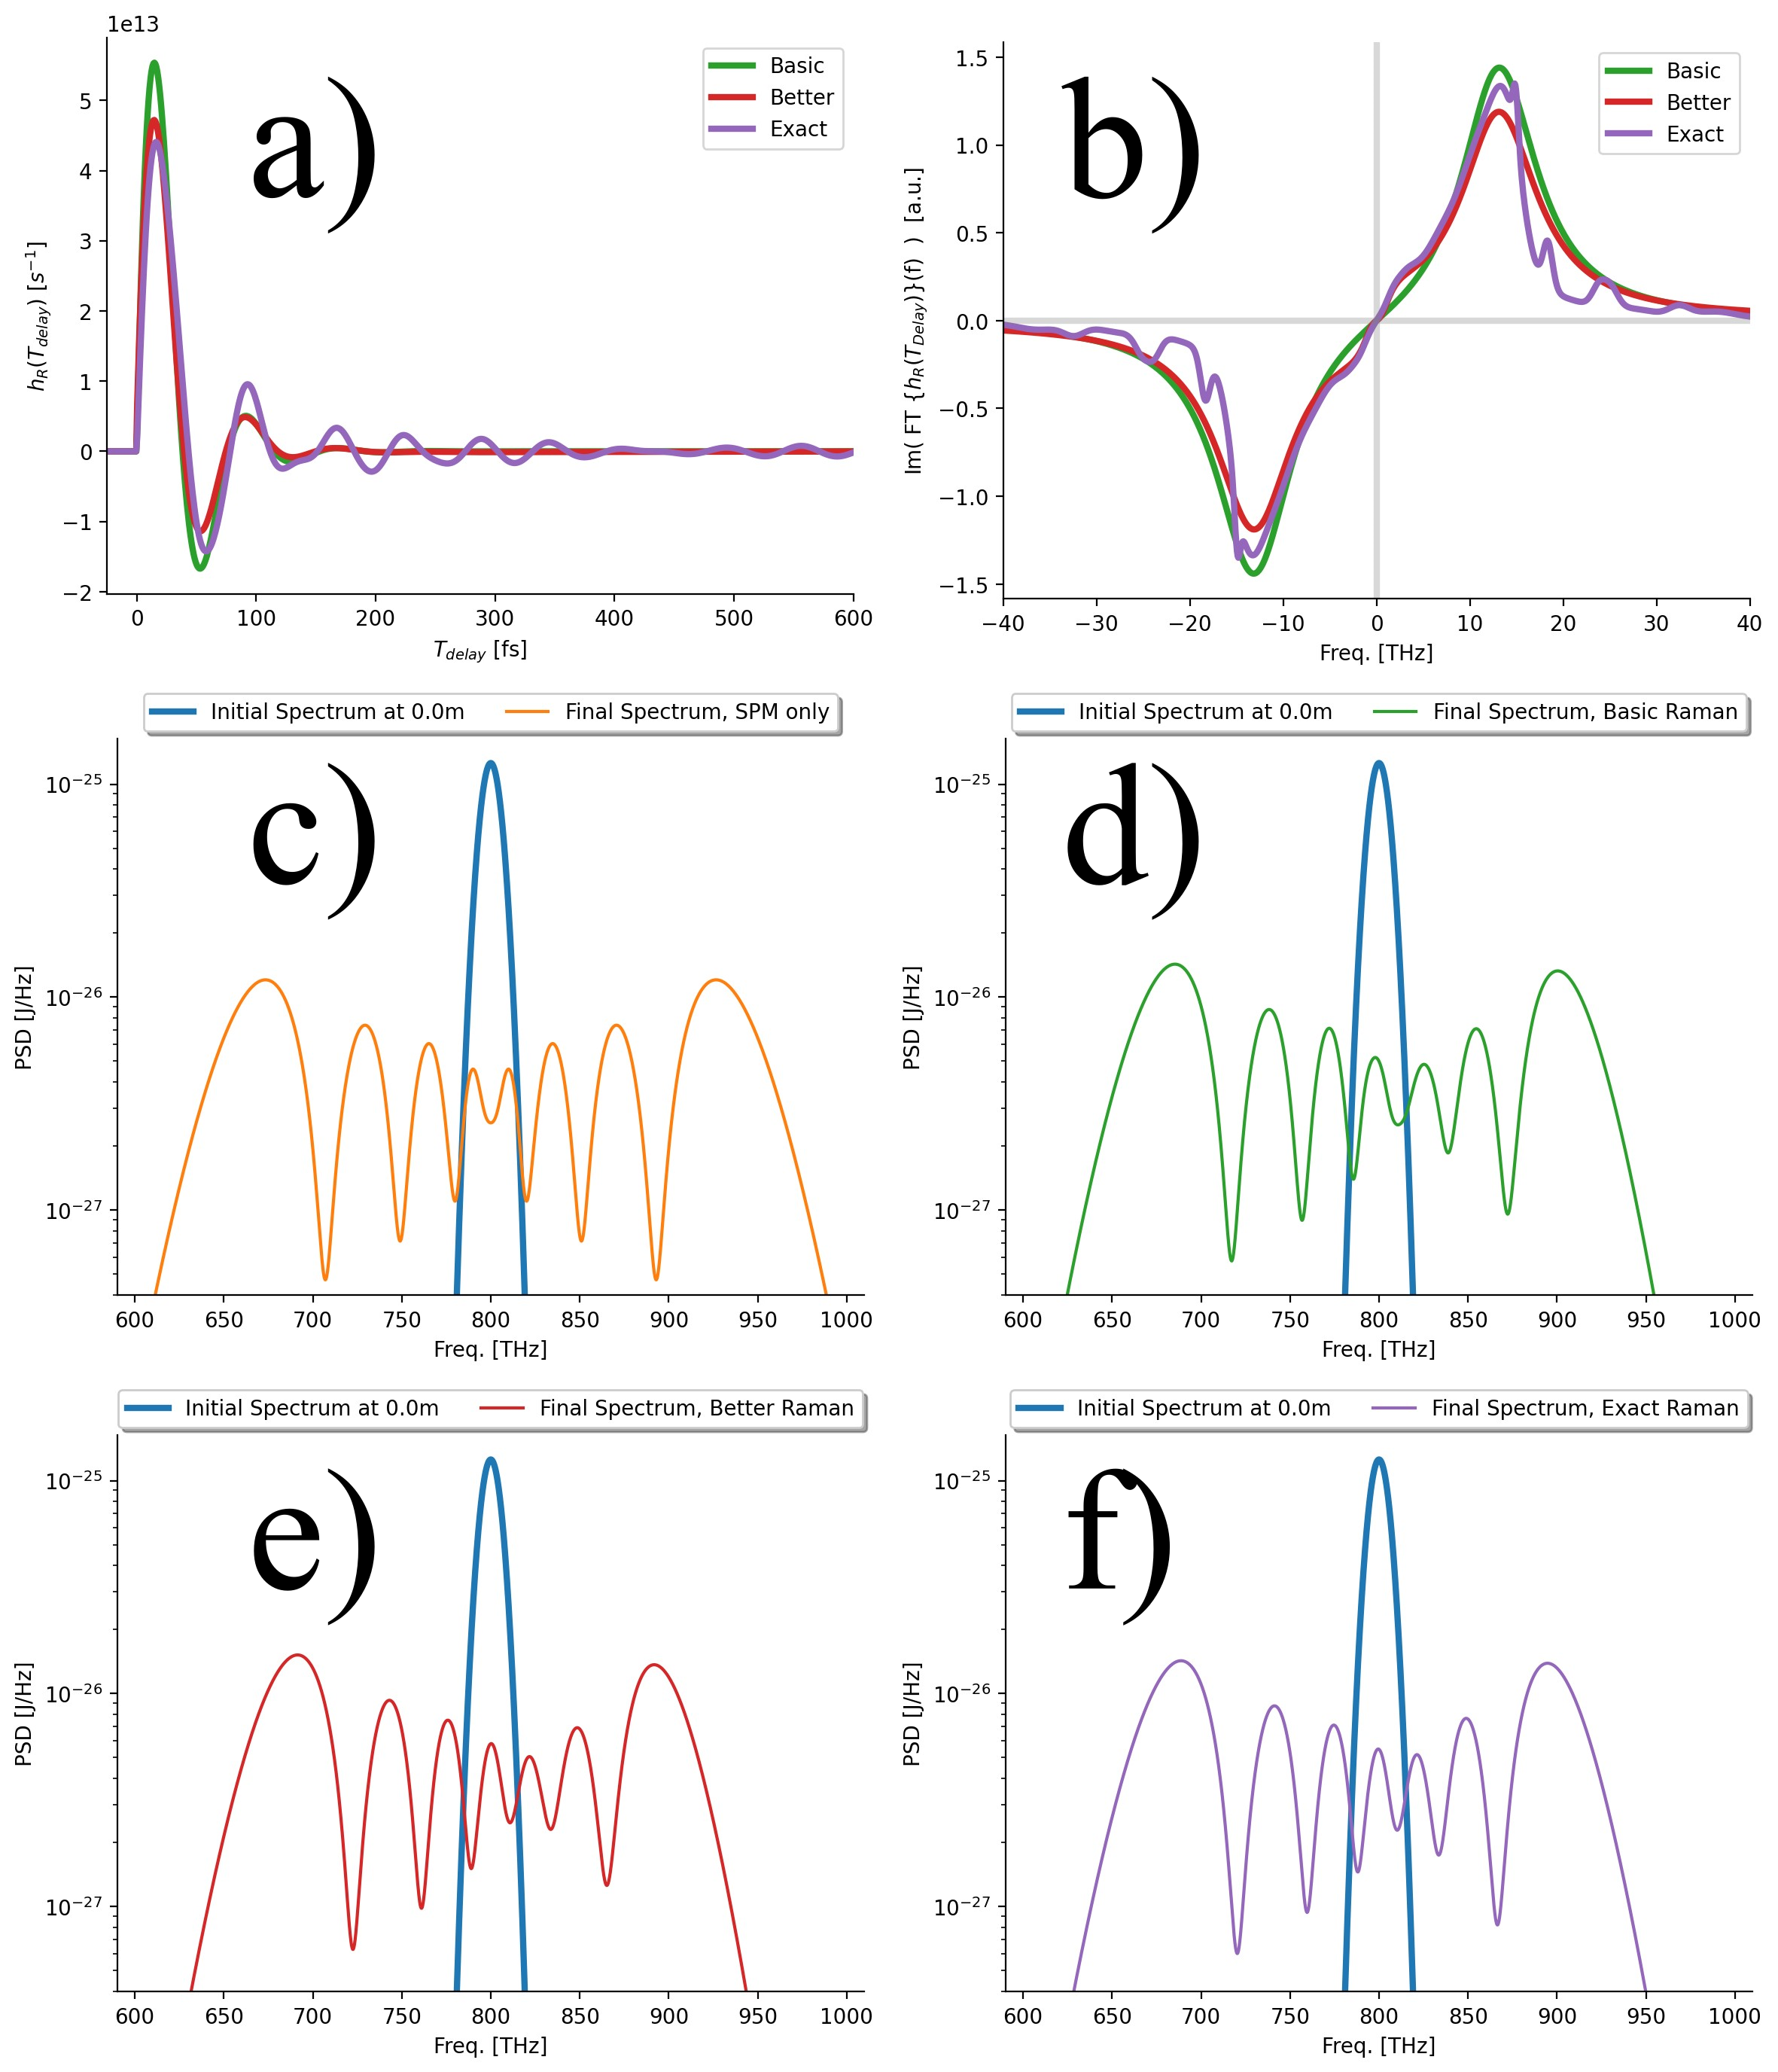
\includegraphics[width=1\linewidth]{figures/Raman_combined.png}
    \caption{a) Eq.~\ref{eq:raman_basic}(绿色)、Eq.~\ref{eq:raman_new}(红色)和 Eq.~\ref{eq:Raman_exact}(紫色)的时域图。) c) 仅受 SPM 影响的脉冲的初始和最终光谱。 d) 受公式 ~\ref{eq:raman_basic} 描述的拉曼效应影响的与 c) 中相同脉冲的初始和最终光谱。e) 与 d) 相同,但 Eq.~\ref{eq:raman_new} f) 与 d) 相同,但 Eq.~\ref{eq:Raman_exact}. 这些图是使用 \href{https://colab.research.google.com/drive/1TqixCGQ51DVwpB3VA6J1XQCpDcf4xwb4?usp=sharing}{这个交互式笔记本}生成的,鼓励读者尝试使用。}
    \label{fig:raman_combined}
\end{figure}






    \chapter{Exotic pulses}
\label{ch:Exotic}

For a fiber, where $\gamma\neq 0$ and $\betag_2\neq 0$, a pulse launched into it can evolve in a number of surprising ways. Essentially, the nonlinearity will change the local frequency of the pulse based on its power profile, while dispersion will cause different frequencies to advance or delay relative to the carrier frequency, which in turn, alters the power profile. This chapter explores the interplay between these two effects for different values of $\gamma$ and $\betag_2$. 


\section{The Fundamental Soliton}
\label{sec:soliton}
Consider a fiber for which $\gamma>0$. As illustrated in Fig.~\ref{fig:chirp_profiles}, this will cause leading(trailing) pulse edges to develop a red(blue) shift. As explained in Sec.~\ref{sec:GVD}, $\betag_2<0$ implies that blue light propagates faster than red light, thus causing the leading(trailing) edge of a pulse will become more blue(red). If $\gamma>0$ makes the front(back) of the pulse more red(blue) based on the instantaneous power profile, while $\betag_2<0$ makes the front(back) more blue(red) according to the 2nd time derivative of the field, it's natural to ask if there exists a pulse envelope, where the two effects balance exactly at every instant, so that the shape of the pulse is unaltered as it propagates forward. For such a pulse, the field envelope should be independent of distance, while the phase should be independent of time, such that
\begin{align}
    \A(z,T) &= V(T)e^{i\phi(z)}
\end{align}
solves 
\begin{align}
\label{eq:NLSE_soliton}
    \partial_z\A &=  -i  \frac{\betag_2}{2}\partial_T^2\A+i\gamma|\A|^2\A.
\end{align}
As explained in \href{https://github.com/OleKrarup123/NLSE-vector-solver/blob/main/TutorialVideos/Soliton-Video/Fundamental_soliton_derivation.pdf}{this derivation}, it can be shown that the solution is
\begin{align}
    \A(z,T) &= \sqrt{\frac{|\betag_2|}{\gamma T_0^2}}\cdot\text{sech}\left(\frac{T}{T_0}\right)\exp\left(i\frac{|\betag_2|}{2T_0^2}z\right),
\end{align}
where $T_0$ is the time at which the field of the pulse has decreased to 64.8\% of its peak value. This stable pulse characterized by a hyperbolic secant envelope is referred to as a "fundamental soliton". See Fig.~\ref{fig:gauss_sech} for a comparison of a Gaussian pulse to a hyperbolic-secant pulse. Note that the peak power of the hyperbolic-secant pulse, $\A_{max}$, must be chosen to exactly equal the characteristic amplitude, $\A_{char}=\sqrt{|\betag_2|/\gamma T_0^2}$, for stable propagation to occur!
\begin{figure}
    \centering
    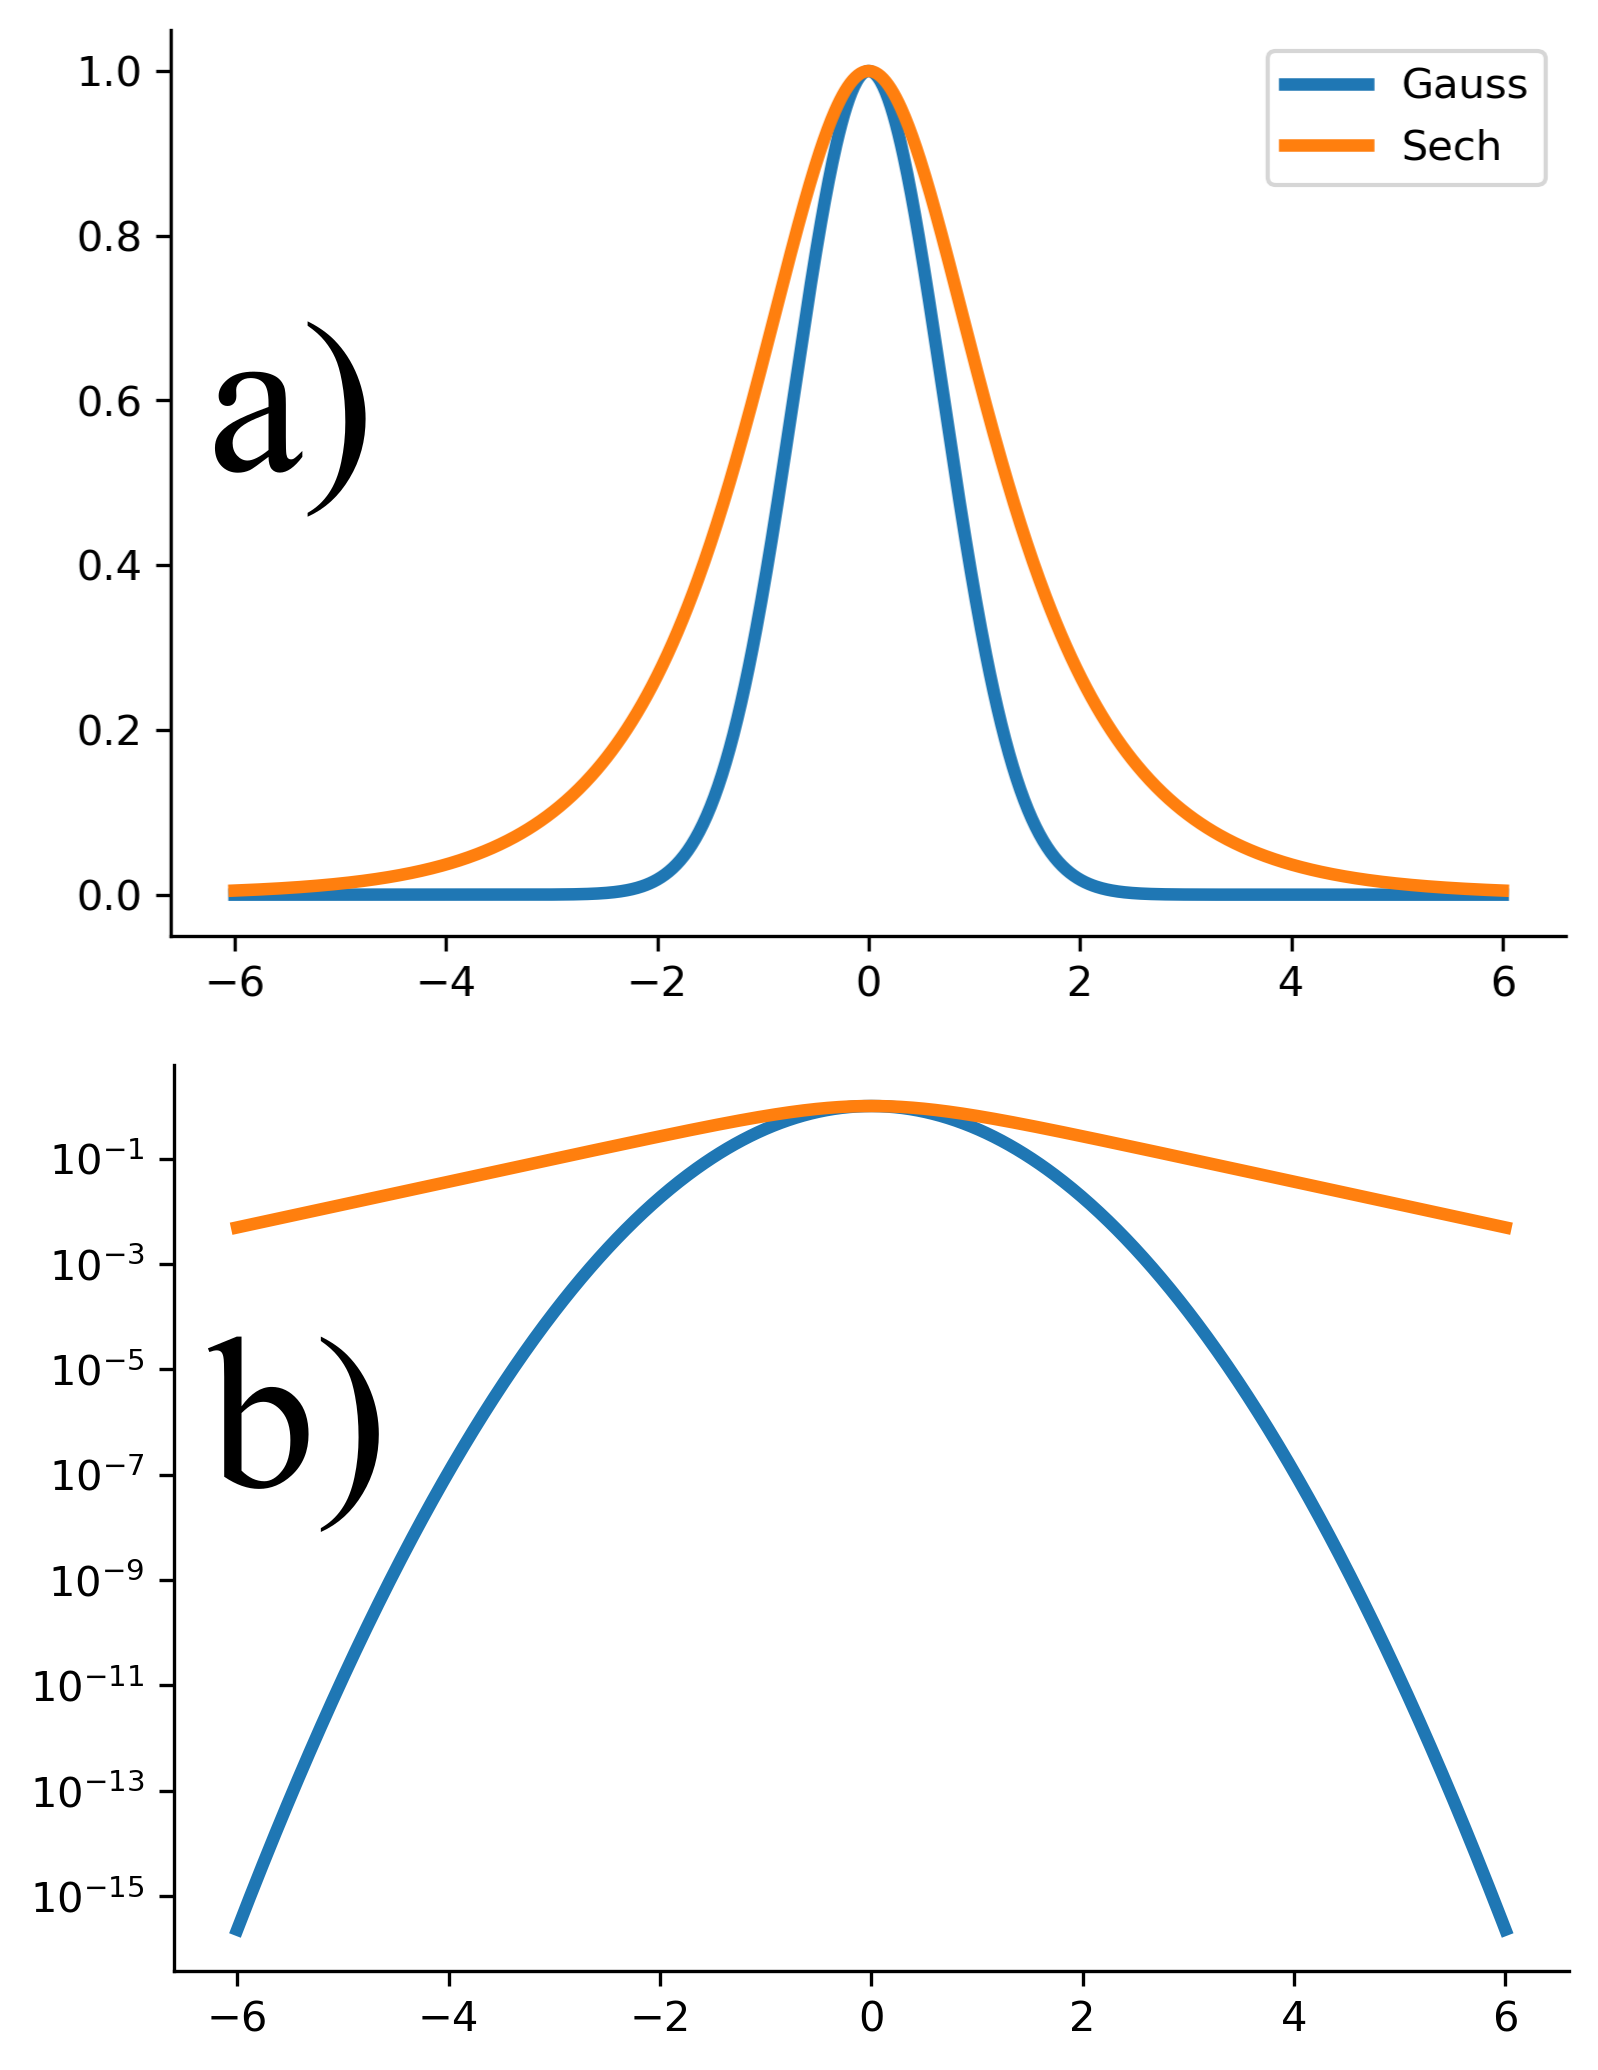
\includegraphics[width=1\linewidth]{figures/gauss_sech_comparison.png}
    \caption{Comparison of a Gaussian pulse to a hyperbolic-secant pulse on a linear scale in a) and a logarithmic scale in b), which emphasizes the comparatively more intense tails of the hyperbolic-secant.  }
    \label{fig:gauss_sech}
\end{figure}
\subsection{Solitons in telecommunications}
As $\gamma>0$ and $\betag_2<0$ in silica fibers for near-infrared frequencies close to 193~THz ($\approx$1550~nm), fundamental solitons were once of great interest in telecommunications because their resistance to dispersion and constant shape reduced inter-symbol interference. However, the same improvements in electronic dispersion compensation mentioned in Subsection~\ref{subsec:ZDF} have rendered the use of solitons for optical fiber communication obsolete. Instead, pulses with a so-called "\href{https://www.youtube.com/watch?v=hCk_cg-OfUQ}{root-raised-cosine}" field envelope are used.   


\section{Higher order Solitons}
If the peak power of the hyperbolic secant pulse smaller than $P_{char}=|\A_{char}|^2=|\betag_2|/\gamma T_0^2$, the nonlinear effect will be too weak compared to dispersion for a fundamental soliton to form. The pulse will thus simply broaden in the time domain as it propagates forward. If the peak power is increased beyond $P_{char}$, the pulse will exhibit "oscillations" as it evolves. For the special case of $\A_{max}$ being an integer multiple of $\A_{char}$, the oscillating soliton evolution will be particularly well-behaved. See Fig.~\ref{fig:Soliton_comparison}~a-b) for an example of the temporal and spectral evolutions of a soliton for which $\A_{max}=3\A_{char}$. See \href{https://youtu.be/KAZ7pCQ-x8Y}{this video tutorial} for more information on solitons in fibers. 

\subsection{Soliton fission}
\label{subsec:fission}
Fundamental- and higher order solitons can be seen as "fixed points" of Eq.~\ref{eq:NLSE_soliton}. However, Eq.~\ref{eq:NLSE_soliton} itself is only an approximation to Eq.~\ref{eq:GNLSE}, which provides a more general description of the physics affecting the propagation of an optical pulse in a dispersive and nonlinear medium. It turns out that the presence of effects other than $\gamma>0$ and $\betag_2<0$ will eventually disturb the evolution of an initially solitonic pulse. In Fig.~\ref{fig:Soliton_comparison}~c-d), the presence of $\betag_3>0$ causes a higher order soliton to "fission" into two less powerful ones at new frequencies due to FWM after propagating a distance of 0.5 meters. Other effects, such as Self-Steepening, the Raman effect or even Modulation Instability caused by optical noise propagating along with an otherwise ideal soliton pulse can similarly give rise to soliton fission. Thus, much like a pencil balanced on its tip, solitonic propagation should be viewed as an unstable equilibrium. See \href{https://youtu.be/tHpIR2Kuxp0}{this video tutorial} for more details on soliton fission.
\begin{figure}
    \centering
    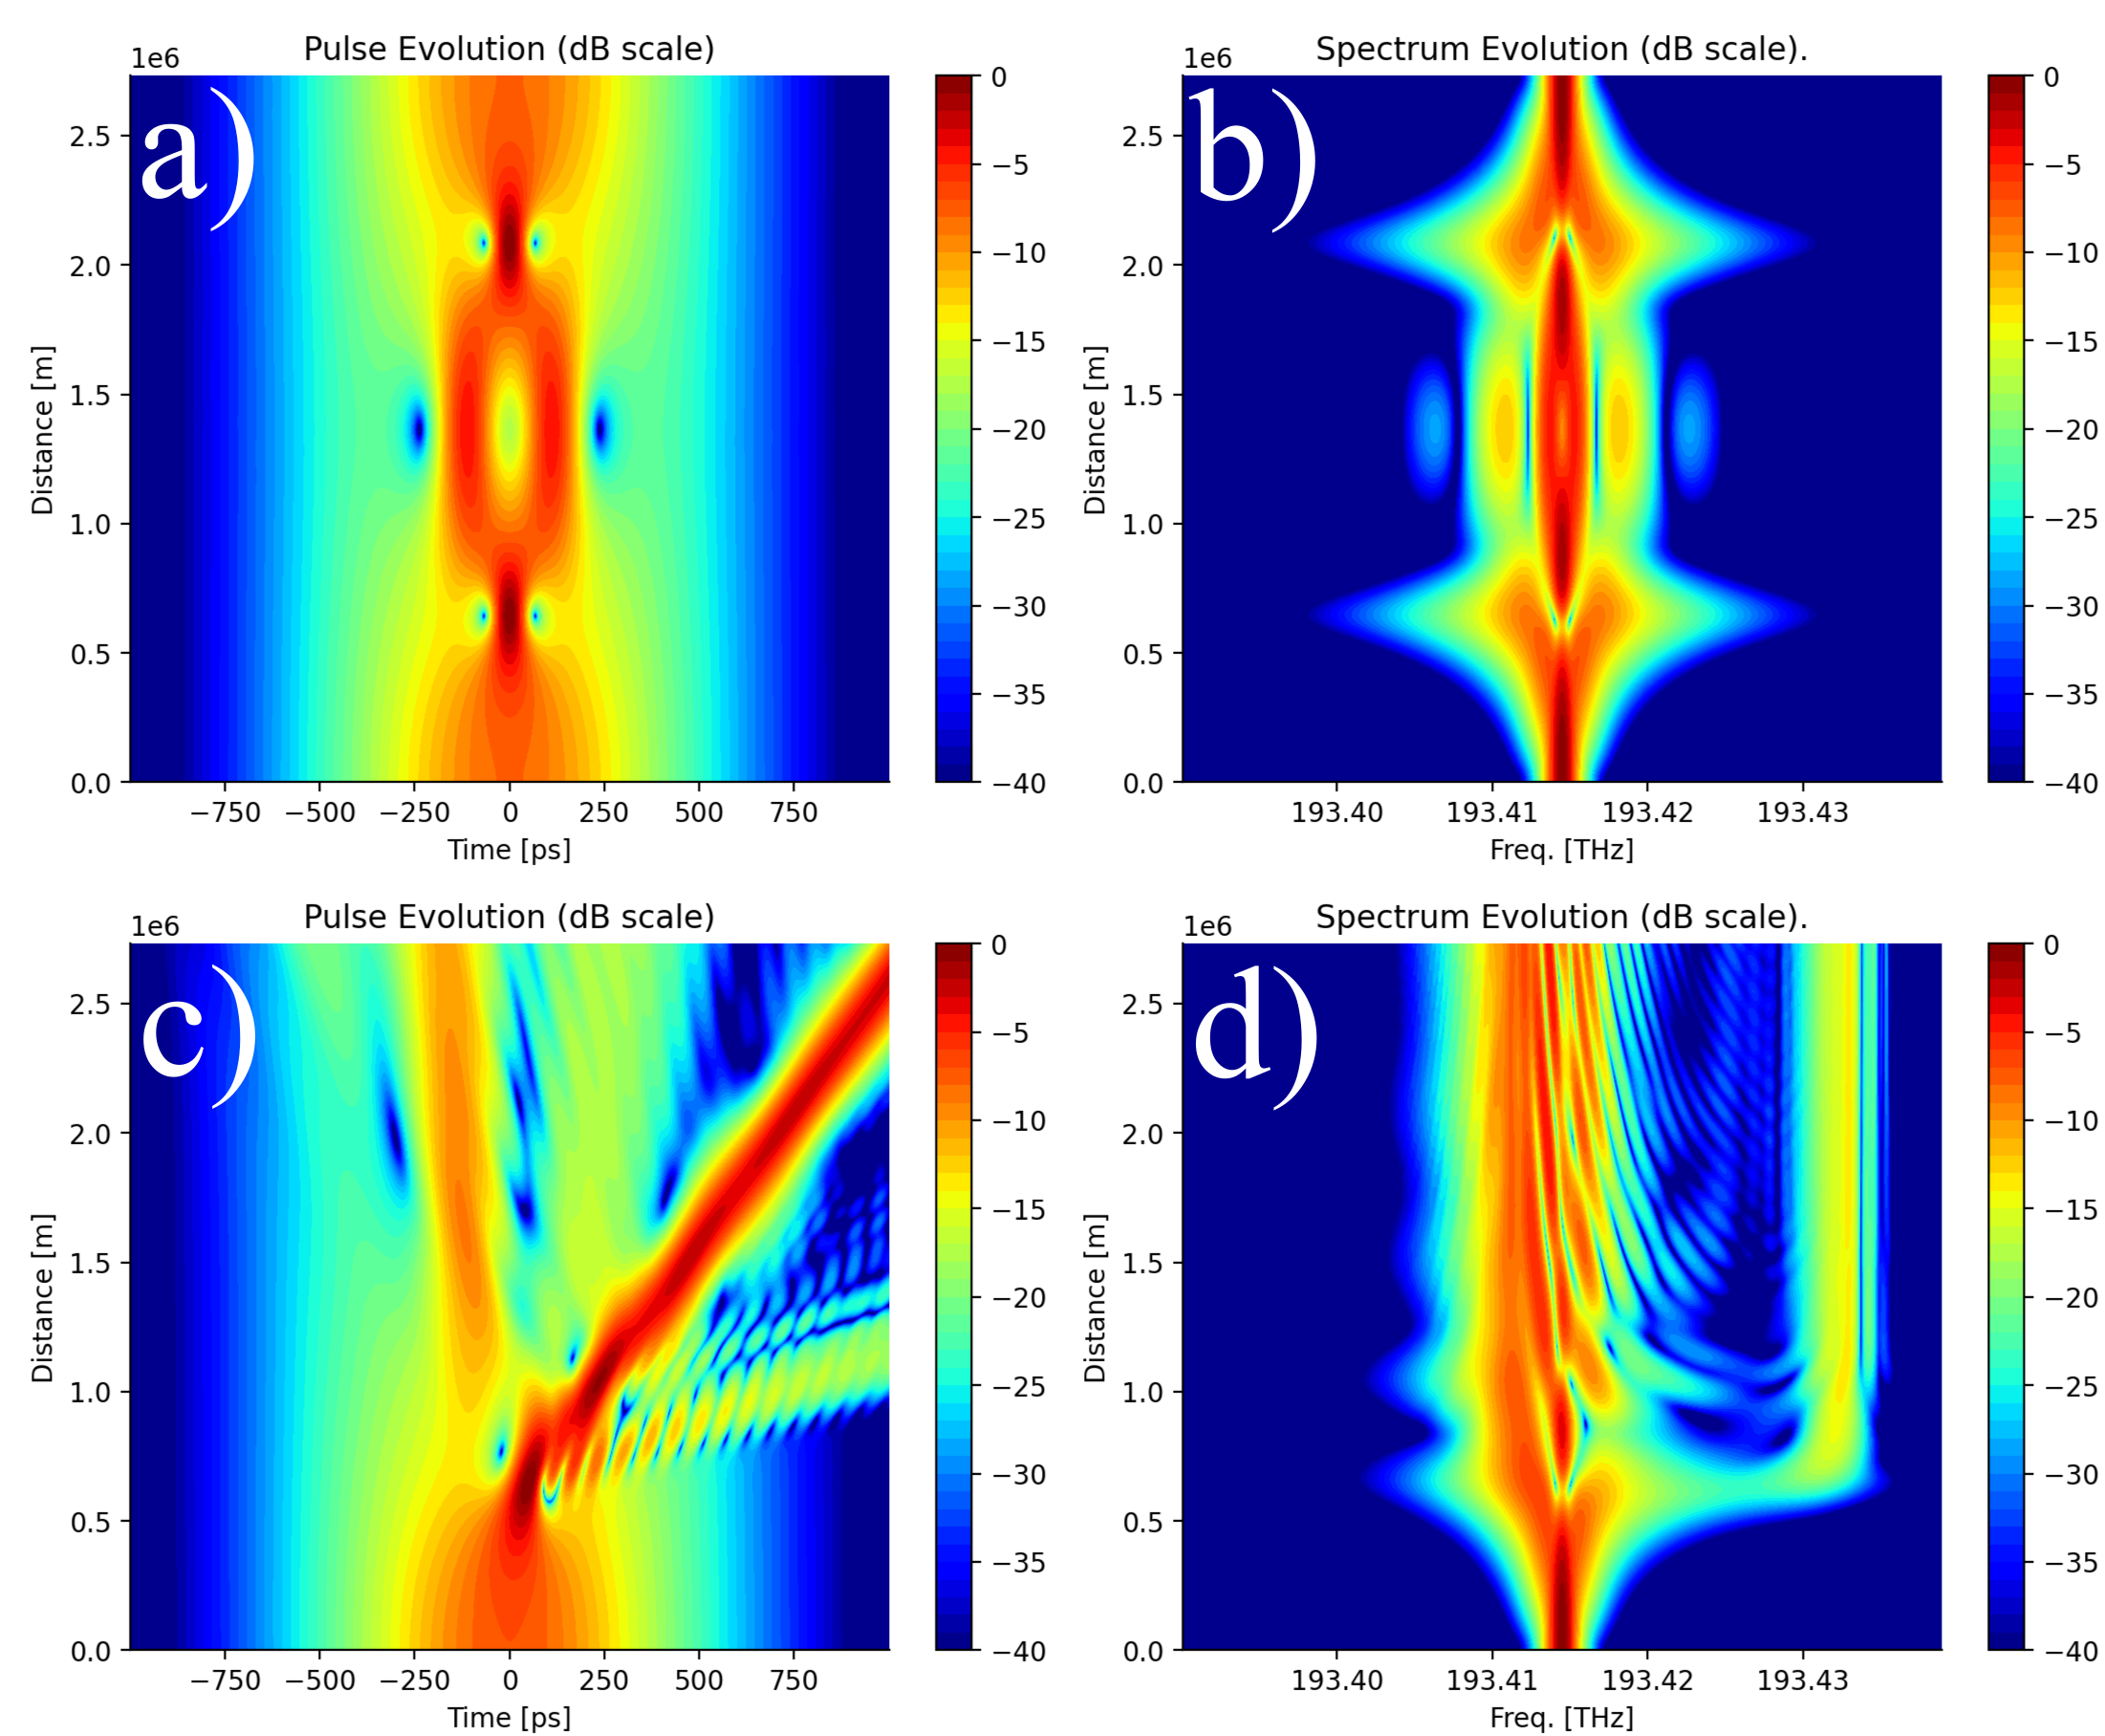
\includegraphics[width=1\linewidth]{figures/Soliton_comparison.png}
    \caption{a) Temporal evolution of an $N=3$ soliton for which $\A_{max}=3\A_{char}=3\sqrt{|\betag_2|/\gamma T_0^2}$. The length of the fiber has been chosen to equal the oscillation period of the soliton. b) Spectrum evolution of the $N=3$ soliton. c-d) Respectively, the temporal and spectral evolutions of the same $N=3$ soliton as in a-b), but where the fiber has $\betag_3>0$, causing the pulse to "fission", thereby illustrating the unstable nature of solitonic propagation. Figures generated using the numerical simulation in \href{https://colab.research.google.com/drive/123pT-IsLWIEZY9XW3-1WzkTXfg1IEkkD?usp=sharing}{this interactive notebook}, which the reader is encouraged to experiment with.}
    \label{fig:Soliton_comparison}
\end{figure}





\section{Optical Wave Breaking}
When an ocean wave approaches a beach, water begins to "pile up" on its leading edge, eventually causing the wave to "break" before crashing onto the shore. A similar phenomenon can be observed with optical waves in nonlinear fibers where $\gamma>0$ and $\betag_2>0$. Instead of the local color-changes from nonlinearity and dispersion balancing as in Sec.~\ref{sec:soliton} when $\betag_2$ was negative, they now "cooperate". The nonlinearity makes the front(back) of the pulse more red(blue) and dispersion causes red(blue) light to move faster(slower) than the carrier. The result is that any pulse will quickly broaden in the time domain. Often, this happens in such a way that power gradually "piles up" in both the front and back of the pulse, leading to steeper power slopes, which generate even larger chirps causing more rapid temporal broadening due to dispersion. When the slope steepness gets sufficiently large, dispersion will "launch" the newly generated frequencies away from the main pulse in a manner analogous to a crashing water wave. Figure~\ref{fig:OWB_and_similariton}~a-b) illustrates this effect called "Optical Wave Breaking" (OWB). While the changes to incident pulses induced by OWB can be detrimental, they can also be beneficial if one desires an optical pulse with steep slopes and approximately constant peak power. See \href{https://youtu.be/XEx6lOf6f40}{this video tutorial} for further details on OWB. 

\subsection{Similaritons}
When $\gamma>0$ and $\betag_2>0$, OWB broadens the pulse in the time domain, thereby reducing its peak power. If, additionally, $\alpha>0$, implying that the pulse is amplified as it moves forward, this loss of peak power is continuously replaced. It turns out that under these circumstances, any input pulse \emph{regardless of its initial shape} will evolve towards a parabolic power envelope as illustrated in Fig.~\ref{fig:OWB_and_similariton}~c) and a linearly changing chirp that goes from red in the front to blue in the back~\cite{Similariton_evolution}. Both the peak power and duration of such a "similarition" will continuously increase with distance as explained in \href{https://youtu.be/ZtWIRaj5VV4}{this video tutorial}. Similaritons can arise in certain optical amplifiers and their linearly changing chirps make them ideal candidates for generating pulses with extremely high peak powers through the Nobel-Prize winning method of chirped pulse compression explained in \href{https://youtu.be/Eh5CHRWFT-M}{this video tutorial}.   

\begin{figure}
    \centering
    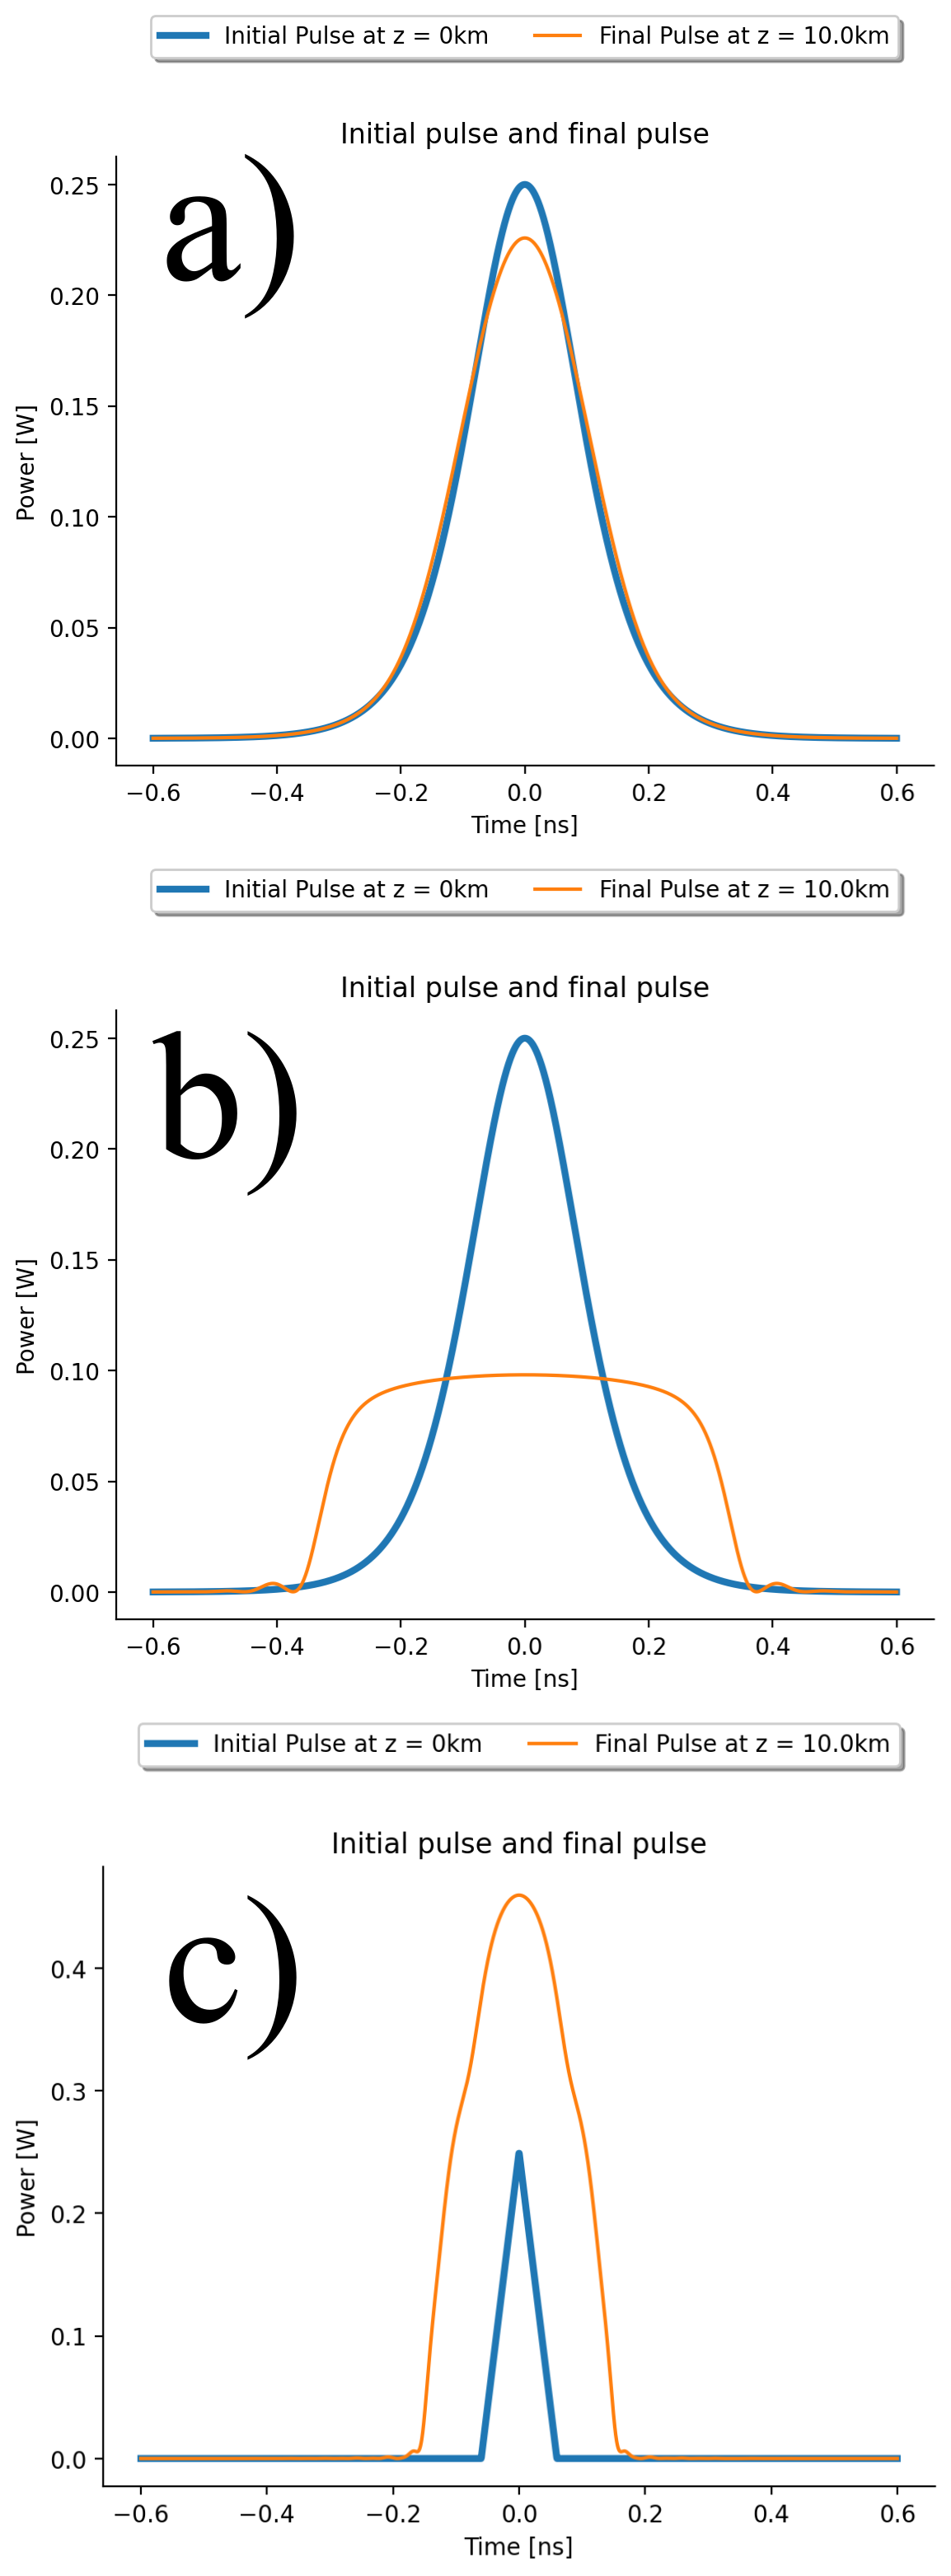
\includegraphics[width=0.5\linewidth]{figures/OWB_and_similariton.png}
    \caption{a) Evolution of a hyperbolic secant pulse through a medium where $\betag_2>0$. b) Evolution of the same pulse as in a) through a medium where $\betag_2>0$ and $\gamma>0$ cause power to "pile up" in the front and back of the pulse, leading to OWB. c) Same conditions as in b), but where $\alpha>0$ causes a triangular pulse to evolve towards a parabola. Figures generated using the numerical simulation in \href{https://colab.research.google.com/drive/1qtMcXElXn4VBntfCgXIGGkyDfiGicElx?usp=sharing}{this interactive notebook}, which the reader is encouraged to experiment with.  }
    \label{fig:OWB_and_similariton}
\end{figure}


\section{Novel Solitons}
\subsection{Dark Solitons} 
Typically, optical pulses consist of a sudden increase in laser power preceded and followed by long durations of zero power. To the naked eye, such a pulse would be a bright flash, like a lamp being briefly switched on in a dark room. Such pulses can propagate stably through a nonlinear medium if the conditions described in Sec.~\ref{sec:soliton} are satisfied. Consider instead what might be called an "anti-pulse" in a nonlinear medium; a high power CW signal, which experiences a brief dip in its power, analogous to a bright lamp that is briefly switched off before being reactivated. It will consist of a decreasing leading edge and an increasing trailing edge. If $\gamma>0$ and $\betag_2>0$, the leading(trailing) edge becomes more blue(red), causing the light there to slow down(speed up). Similarly to Sec.~\ref{sec:soliton}, one can calculate that the field envelope for which nonlinearity and dispersion cancel exactly is a hyperbolic tangent, thereby leading to a stably propagating "Dark Soliton" described by 
\begin{align}
    \A(z,T) = \A_{char}\tanh\left(\frac{T}{T_0}\right)\exp\left(i\frac{|\betag_2|}{T_0^2}z \right).
\end{align}
See \href{https://youtu.be/MrNfI1_eTZ0}{this video tutorial} for more information on Dark Solitons.


\subsection{Raman Solitons}
If the Raman effect, which shifts the spectrum of a pulse towards lower frequencies, is present in a nonlinear medium where $\betag_2<0$, a "Raman Soliton" can form. This soliton retains the shape of its envelope, but undergoes a constant red-shift and obtains an increasingly large time delay since $\betag_2<0$ implies that red light moves more slowly than blue light as illustrated in Fig.~\ref{fig:dark_and_raman}c-d). Raman solitons often arise after soliton fission of pulses with durations on the scale of tens of femtoseconds. See \href{https://www.youtube.com/watch?v=K33YUfegL1w}{this video tutorial} for an explanation of Raman solitons.

\begin{figure}
    \centering
    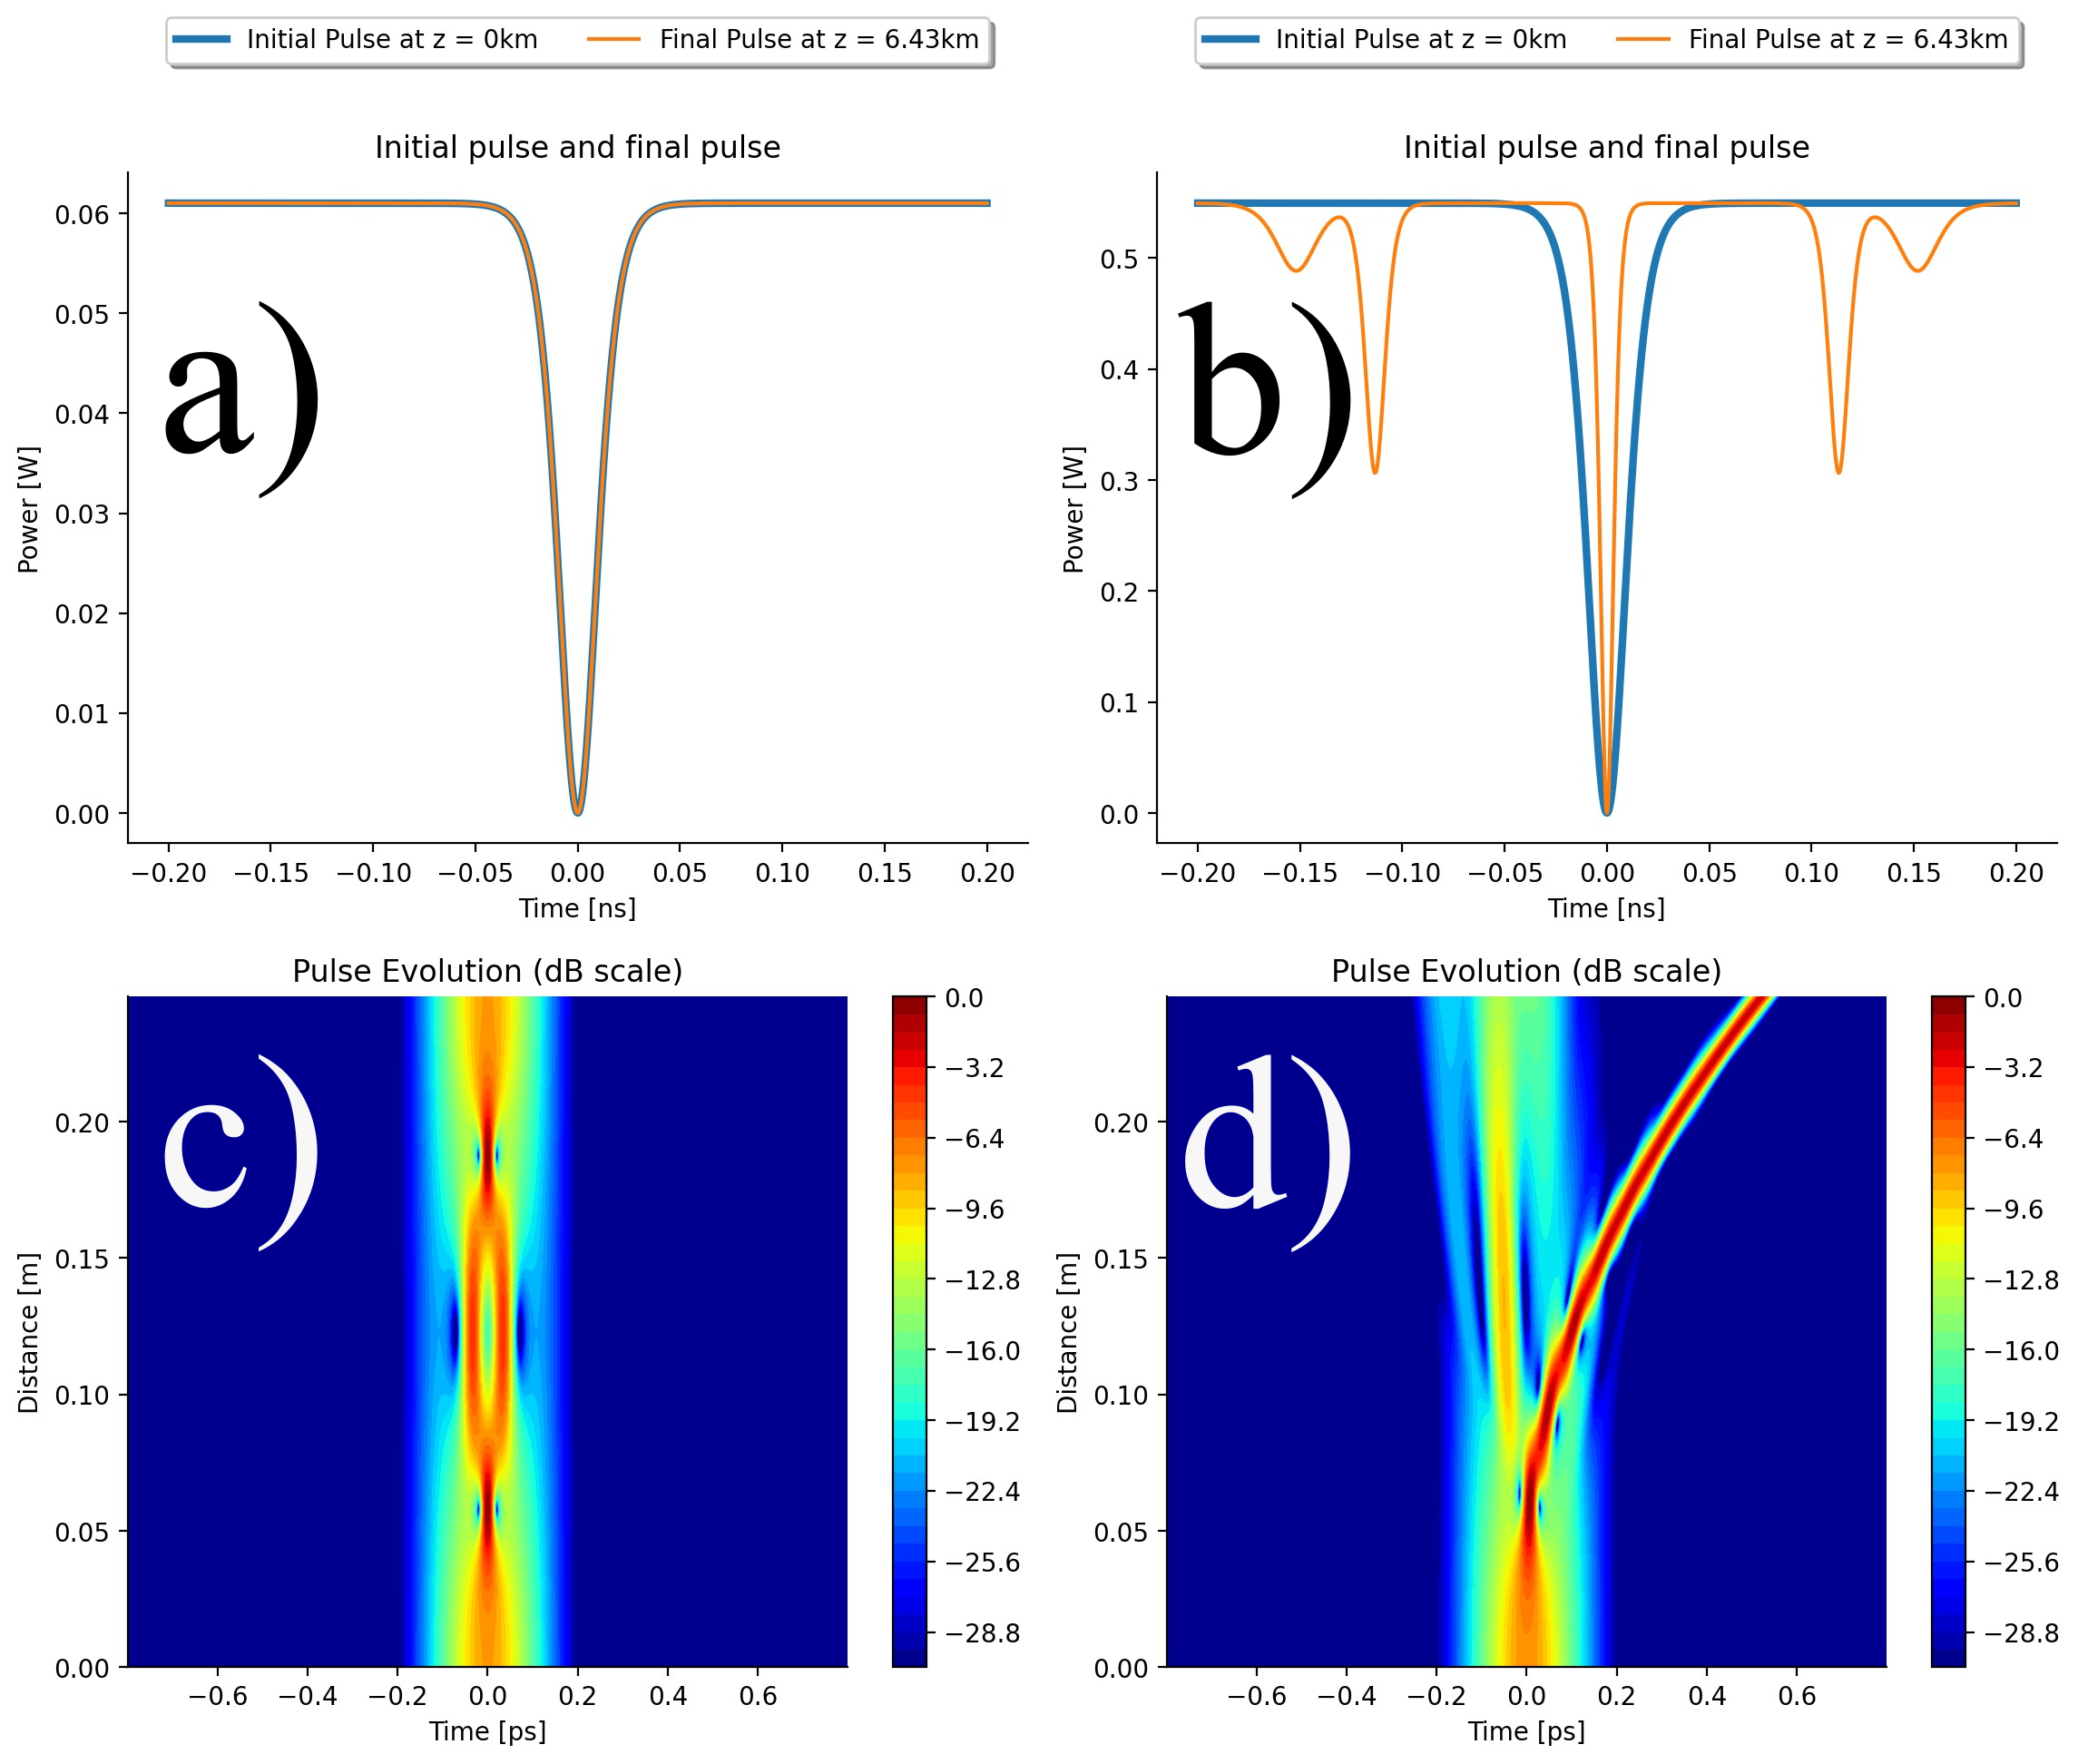
\includegraphics[width=1\linewidth]{figures/dark_and_raman_soliton_combined.png}
    \caption{a) Fundamental dark soliton propagating stably through a medium where $\betag_2>0$ and $\gamma>0$. b) An N=3 dark soliton propagating through the same medium as in a) Instead of stable propagation, the central dip gives rise to additional ones. c) An N=3 soliton propagating through a medium where $\betag_2<0$ and $\gamma>0$. d) The same pulse as in c) propagating through the same medium except the Raman effect described by Eq.~\ref{eq:raman_basic} is taken into account, causing soliton fission and a self-redshifting Raman soliton to arise. Figures generated using \href{https://colab.research.google.com/drive/1qtMcXElXn4VBntfCgXIGGkyDfiGicElx?usp=sharing}{this interactive notebook}, which the reader is encouraged to experiment with.}
    \label{fig:dark_and_raman}
\end{figure}

\subsection{Vector Solitons}
In Sec.~\ref{Sec:XPM}, it was shown that two distinct frequencies of light can affect each others phases through the nonlinearity. Similarly, two different polarizations of light propagating in a nonlinear medium can affect each other's phases. Using a vectorial version of Eq.\ref{eq:GNLSE} where $\gamma>0$, $\betag_2<0$, and where the refractive index is different for light polarized along the x- and y-axes of the medium, one can obtain analytical expressions for so-called "Vector Solitons". The special cases for which this is possible turn out to be circularly polarized light and light polarized linearly at $45^{o}$ to the x-axis~\cite{AGRAWAL_CH6_POL}.







    \chapter{Supercontinuum Generation}
\label{ch:supercontinuum}

Previous chapters explained individual linear and nonlinear effects and the interplay of a limited number of them. A summary of their impacts is provided in Tab.~\ref{tab:NL_summary}. For high power pulses with carrier frequencies where $\betag_2\lesssim 0$ and $\gamma>0$ for a given medium as well as durations below approximately 100~fs, all of the listed effects may be present simultaneously. In this case, the evolution of the pulse may be highly non-trivial and broaden its spectrum by ten to twenty times its initial bandwidth~\cite{supercontinuum_original_paper}. This chapter presents an example of supercontinuum generation and explains how this process can be understood in terms of the previously presented effects.   

\begin{table}[]
\begin{adjustwidth}{-2cm}{}
\begin{tabular}{ccccc}
\hline
\textbf{Effect}       & \textbf{Time domain}                                                                                      & \textbf{Spectrum}                                                                                           & \textbf{Significant for}                                                                           & \textbf{Relevance}                                                                                                       \\ \hline
$\alpha>0$            & Increase power.                                                                                           & Increase power.                                                                                             & Amplifiers                                                                                         & \begin{tabular}[c]{@{}c@{}}NL effects highly \\ power dependent.\end{tabular}                                            \\ \hline
$\beta_2<0$           & \begin{tabular}[c]{@{}c@{}}Broadening with \\ blue(red)  light in \\ front(back).\end{tabular}            & \begin{tabular}[c]{@{}c@{}}Quadratic change \\ in phase with \\ distance from \\ carrier freq.\end{tabular} & \begin{tabular}[c]{@{}c@{}}Short NIR pulses \\ in silica.\end{tabular}                             & \begin{tabular}[c]{@{}c@{}}NL effects significant \\ when $\beta_2+\gamma P\approx 0$.\end{tabular}                      \\ \hline
$\beta_3$             & \begin{tabular}[c]{@{}c@{}}Delays or advances \\ non-carrier freqs. \\ depending on sign.\end{tabular}    & \begin{tabular}[c]{@{}c@{}}Cubic change in \\ phase with distance \\ from carrier freq.\end{tabular}        & \begin{tabular}[c]{@{}c@{}}Carrier freqs. \\ close to ZDF.\end{tabular}                            & \begin{tabular}[c]{@{}c@{}}Different freqs. \\ overlapping in time \\ domain cause FWM. \\ Soliton fission.\end{tabular} \\ \hline
Self Phase Modulation & \begin{tabular}[c]{@{}c@{}}Red(blue)-shift on \\ leading(trailing)edges.\end{tabular}                     & \begin{tabular}[c]{@{}c@{}}Symmetric \\ broadening.\end{tabular}                                            & High power pulses                                                                                  & \begin{tabular}[c]{@{}c@{}}Most basic NL effect. \\ First to "kick in" as \\ power is increased.\end{tabular}            \\ \hline
Self Steepening       & \begin{tabular}[c]{@{}c@{}}Pulse peak delayed \\ to later times causing \\ steep back slope.\end{tabular} & \begin{tabular}[c]{@{}c@{}}Broadening skewed \\ towards higher \\ frequencies.\end{tabular}                 & \begin{tabular}[c]{@{}c@{}}Pulses with short \\ duration compared \\ to carrier freq.\end{tabular} & \begin{tabular}[c]{@{}c@{}}Small correction on \\ top of SPM.\\ Soliton fission.\end{tabular}                            \\ \hline
Raman                 & Red-shift at pulse peak.                                                                                  & \begin{tabular}[c]{@{}c@{}}Broadening skewed \\ towards lower \\ frequencies.\end{tabular}                  & \begin{tabular}[c]{@{}c@{}}Extremely short \\ pulses on the scale \\ of 10-100fs.\end{tabular}     & \begin{tabular}[c]{@{}c@{}}Raman red-shift can \\ exceed SPM \\ broadening.  \\ Soliton fission.\end{tabular}            \\ \hline
\end{tabular}
\caption{Summary of the impacts of different linear and nonlinear effects.}
\label{tab:NL_summary}
\end{adjustwidth}
\end{table}
\section{Case study}
To simulate the generation of a supercontinuum, the values in Tab.~\ref{tab:SC_params} were used. The resulting supercontinuum is presented in Fig.~\ref{fig:SC_combined}. The spectrum in Fig.~\ref{fig:SC_combined} c) indicates that the pulse undergoes SPM during the first 1~m of propagation, while Fig.~\ref{fig:SC_combined} b) indicates that soliton fission occurs immediately afterwards. The high-power pulse with a much smaller duration that walks off parabolically towards later times is a Raman soliton that continuously red-shifts itself. The low-power light that "walks off" linearly towards later times is most likely FWM generated when the fissioned soliton overlaps with the remnants of the initial pulse. See \href{https://youtu.be/-GDsMDpC3oA}{this video tutorial} for an in-depth analysis of the properties of this supercontinuum.

\begin{table}[]
\centering
\begin{tabular}{cc}
\textbf{Parameter}                      & \textbf{Value}                                  \\ \hline
N time points                           & $2^{14}$                                          \\
Time resolution {[}fs{]}                & 1.8                                             \\\hline
Pulse type                              & Sech                                            \\
Duration {[}fs{]}                       & 166.79                                          \\
Peak Power {[}W{]}                      & 50                                              \\
Carrier freq. {[}THz{]}                 & 282.823 (=1060~nm)                         \\\hline
$\alpha$ {[}dB/km{]}                    & 0                                               \\
$\betag_2$ {[}s\textasciicircum{}2/m{]} & -3.051721e-27                                   \\
$\betag_3$ {[}s\textasciicircum{}3/m{]} & 7.29029e-41                                     \\
$\betag_4$ {[}s\textasciicircum{}4/m{]} & -1.08817e-55                                    \\
$\betag_5$ {[}s\textasciicircum{}5/m{]} & 2.8941e-70                                      \\
$\betag_6$ {[}s\textasciicircum{}6/m{]} & 4.8348e-89                                      \\
$\betag_7$ {[}s\textasciicircum{}7/m{]} & -1.1464e-113                                    \\
$\betag_8$ {[}s\textasciicircum{}8/m{]} & 1.8802e-128                                     \\
$\betag_9$ {[}s\textasciicircum{}9/m{]} & -1.5054e-143                                    \\
$\gamma$ {[}1/W/m{]}                    & 0.09                                            \\
Self-Steepening                         & ON                                              \\
Raman model                             & Eq.~\ref{eq:raman_basic}
\end{tabular}
\caption{Simulation parameters used for generating a supercontinuum taken from~\cite{supercontinuum_paper}}
\label{tab:SC_params}
\end{table}

\begin{figure}
    \centering
    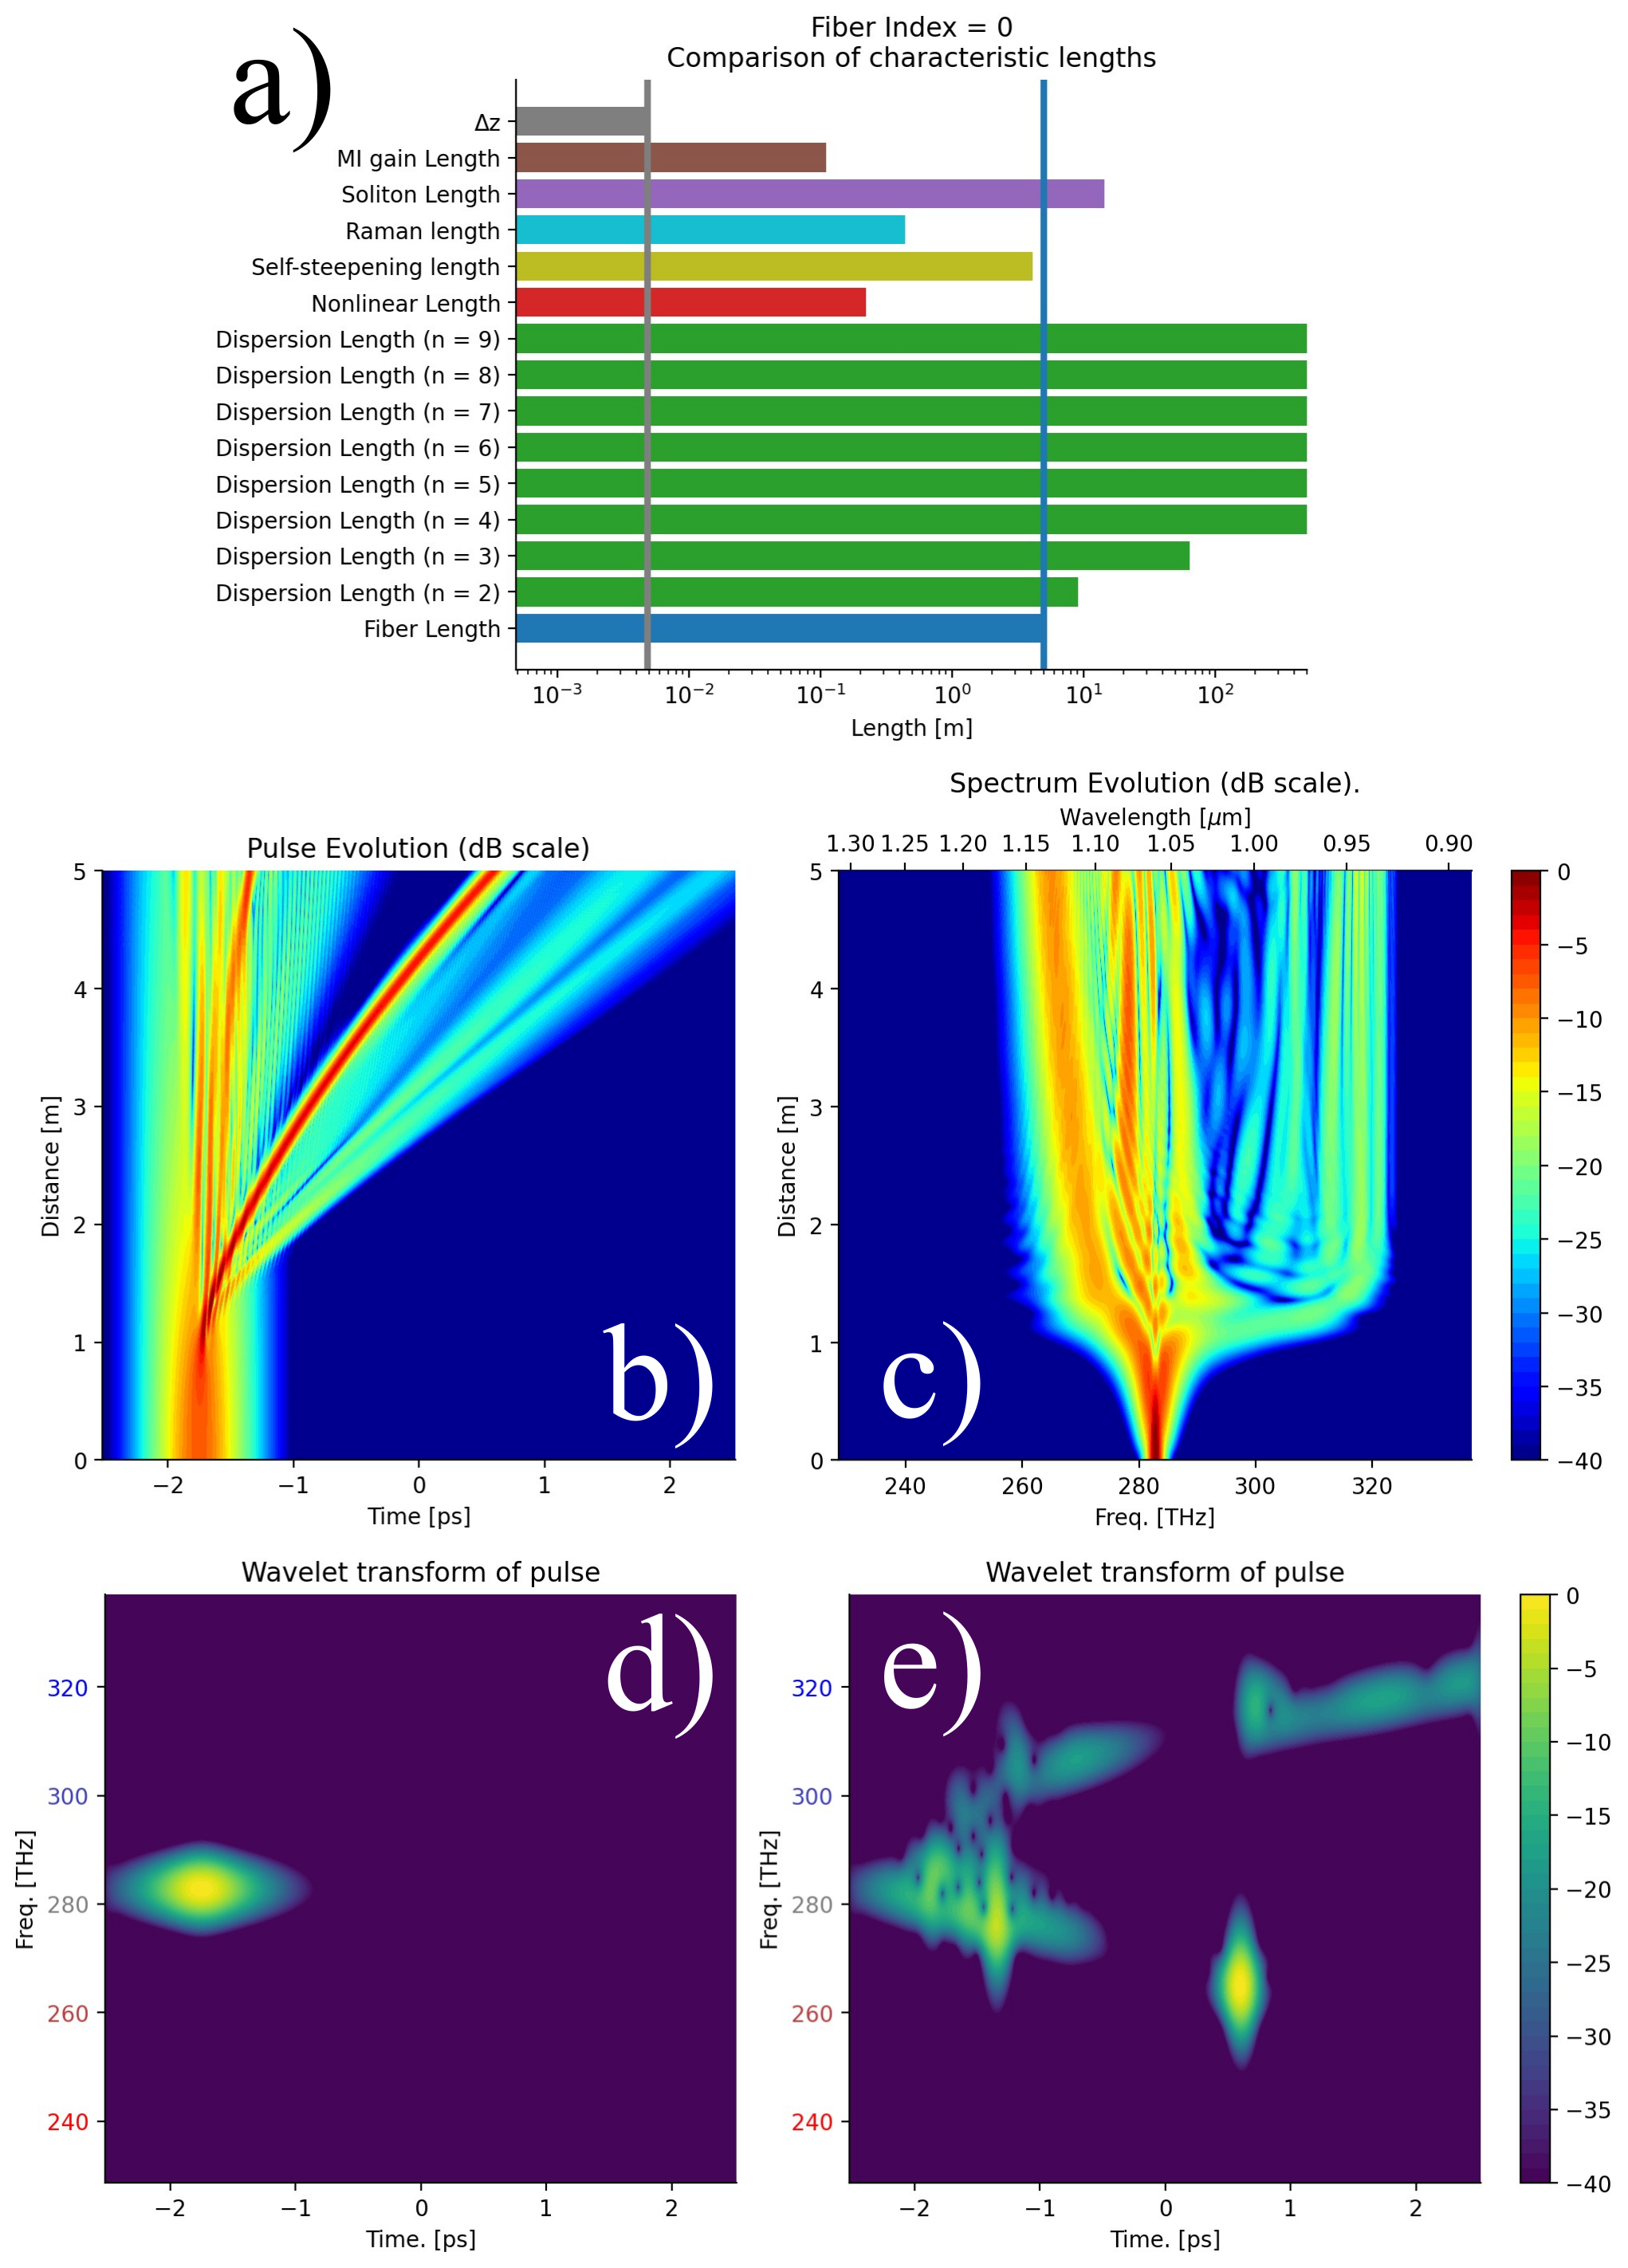
\includegraphics[width=0.9\linewidth]{figures/SC_combined.png}
    \caption{a) Comparison of the characteristic lengths resulting from the parameters listed in Tab.~\ref{tab:SC_params}. Effects with short characteristic lengths are expected to become significant first. b) Temporal evolution of the pulse showing soliton fission at a distance of around 1~m followed by FWM and the generation of a Raman soliton walking off to later times. c) Spectral evolution of the pulse. d) Initial spectrogram of the pulse at z=0m. e) Final spectrogram at z=5m. The "parabolic" shape arises because $\betag_3>0$ ensures that both red and blue light experience time delays compared to the carrier. The bright spot at (0.75~ps, 265~THz) is a Raman soliton. Figures generated using the numerical simulation presented in \href{https://colab.research.google.com/drive/1HvA8F8yzEq-9fahuI4z2KhT-YhdRAXgt?usp=sharing}{this interactive notebook}, which the reader is encouraged to experiment with. }
    \label{fig:SC_combined}
\end{figure}

\section{Your turn!}
To further explore the properties of the supercontinuum modelled in Fig.~\ref{fig:SC_combined}, open the \href{https://colab.research.google.com/drive/1HvA8F8yzEq-9fahuI4z2KhT-YhdRAXgt?usp=sharing}{notebook} used for generating it, try the following experiments and explain how/why the evolution of the pulse and its spectrum are different. Before starting any experiment, write down a prediction of how you expect the simulation result to be altered, so you can compare with the actual result. Note that you should "reset" the parameters to the default values before each experiment:

\begin{enumerate}

\item \textbf{No nonlinearity}. The presented simulation uses $\gamma>0$. Change this to $\gamma=0$. Does the result indicate that nonlinearity has a large impact on the time evolution of the pulse?

\item \textbf{No Self-Steepening}. The presented simulation models the impact of self-steepening. Turn this effect off and asses if doing so had a significant impact.

\item \textbf{Negative $\alpha$}. The presented simulation uses $\alpha=0$. Change this to $\alpha=-1$~dB/m. 



\item \textbf{Positive $\betag_2$}. The presented simulation uses $\betag_2<0$. Change the sign of $\betag_2$ so it becomes positive. 



\item \textbf{Only $\betag_2<0$}. The presented simulation uses $\betag_n\neq0$ for $n>2$. Set $\betag_n = 0$ for $n>2$, run the simulation and explain why the evolution of the pulse and its spectrum has changed. 

\item \textbf{Negative $\betag_3$}. The presented simulation uses $\betag_3>0$. Change the sign of $\betag_3$ so it becomes positive. Note that you may want to change the sign of the time offset from -1.75~ps to +1.75~ps to ensure proper graphing of the time evolution. Can you explain why a Raman soliton does not arise when $\betag_3<0$? HINT: Compute the zero dispersion frequency using Eq.~\ref{eq:ZDF} and consider how it changes when the sign of $\betag_3$ is flipped.


\item \textbf{Alter the Raman model}. The presented simulation uses Eq.~\ref{eq:raman_basic} to model the impact of the Raman effect. Follow the hints in the notebook and use Eq.~\ref{eq:raman_new}, Eq.~\ref{eq:Raman_exact} or $f_R=0$ instead.  
\end{enumerate}
    \chapter{推荐资料}
\label{ch:material}
以下是关于光学、电子学和通信领域的有用且易获取的资源列表。

\section{光学}

\subsection*{光子学要素}
这本由伊豆香敬教授编写的教科书,介绍了实际光学器件背后的理论,涵盖了广泛的话题。特别推荐其对掺铒光纤放大器(EDFA)增益和噪声特性的讨论,EDFA是现代光学和电信中不可或缺的工具。

\subsection*{现代光学讲座,帕尔塔·罗伊·乔杜里教授}
这系列\href{https://www.youtube.com/watch?v=2WiMeh1Dxl8&list=PLbRMhDVUMngePMuAGeAUeGVuZffTFY-5i}{60个免费视频讲座}涵盖了麦克斯韦方程、偏振和双折射等基础内容,还包括波导和电光调制器等器件的更高级主题。强烈推荐,因其结构良好且数学推导严谨,涵盖了所有描述的主题。

\subsection*{非线性光学讲座,萨穆德拉·罗伊教授}
这系列\href{https://www.youtube.com/watch?v=EiIDScj124Q&list=PLbRMhDVUMngfBwyonVP8VIsabtnsV3GVv}{60个免费视频讲座}首先讲解了线性光学中的基本概念,然后从麦克斯韦方程出发,详细推导了二阶和三阶非线性效应。讲解了二次谐波生成(SHG)、差频生成(DFG)、光学参量振荡器(OPO)以及一些超出本教材范畴的现象。特别推荐其对$\chi^{(2)}$和$\chi^{(3)}$非线性对称性和张量性质的解释。

\subsection*{非线性光纤光学}
这本由戈温德·P·阿格拉瓦尔编写的教科书详细解释了方程~\ref{eq:GNLSE}背后的数学原理,并且频繁参考实验结果。强烈推荐其对涉及偏振、受激布里渊散射和新型光纤的高级现象的深入讨论。

\subsection*{麻省理工学院“激光与光学演示”讲座系列}
由沙乌尔·以色基尔教授主讲的\href{https://www.youtube.com/watch?v=1cEXNLP5uE0&list=PL4E7FAAD67B171EBC}{49个免费视频讲座},包含了光学基本效应的实践演示,如偏振、干涉和衍射,演示内容基于自由空间光学。强烈推荐,因其系统的实验设计。

\subsection*{国际参数非线性光学学校讲座}
这系列\href{https://www.youtube.com/@ispnlo9041/videos}{44个免费视频讲座}由非线性光学领域的专家主讲。强烈推荐,因其涵盖了通常在普通课程中未涉及的高级主题。

\subsection*{Les' 实验室}
这个\href{https://www.youtube.com/@LesLaboratory/videos}{YouTube频道}专注于激光技术的实际演示,包括染料激光器、光谱仪、电光调制器、SHG以及超连续谱生成等。强烈推荐,因其对相关效应的直观演示和对操作光学器件所需电子学的详细解释。

\subsection*{YourFavouriteTA}
这个\href{https://www.youtube.com/@yourfavouriteta/videos}{YouTube频道}由本教材的作者主讲,通过实际实验、理论推导和数值模拟解释非线性光学。该频道旨在通过直观的解释,帮助观众理解通常由复杂方程描述的线性和非线性过程。

\section{电子学}

\subsection*{The Signal Path}
这个\href{https://www.youtube.com/@Thesignalpath/videos}{YouTube频道}专注于电源、信号发生器、探测器、示波器、频谱分析仪和其他常见的科学和工业实验室设备的实际实验、拆解和维修。特别推荐其关于射频(RF)设备的视频。

\subsection*{EMPossible}
这个\href{https://www.youtube.com/@empossible1577/playlists}{YouTube频道}聚焦于电磁理论的基础以及射频波导、半导体能带结构和有限元分析等高级话题。强烈推荐,因其覆盖了广泛的概念,并提供了优秀的插图和精简的教程。

\subsection*{Keysight 电子学教程}
Keysight电子设备公司的\href{https://www.youtube.com/@KeysightLabs/videos}{YouTube频道},包含了针对电信号测量的解释。特别推荐,因为该频道专注于示波器,这对于通过光电二极管测量功率随时间变化并可视化是常用工具。

\subsection*{Rohde\&Schwarz 电子学教程}
这个由电子设备公司Rohde\&Schwarz制作的\href{https://www.youtube.com/watch?v=rUDMo7hwihs&list=PLKxVoO5jUTlvsVtDcqrVn0ybqBVlLj2z8}{YouTube播放列表}提供了关于电气设备和信号的测量和表征的深入教程,涵盖了功率、相位噪声、放大器噪声因子等内容。许多这些概念可以很好地转移到光学领域。

\section{通信}

\subsection*{Ian Explains}
这个\href{https://www.youtube.com/@iain_explains/videos}{YouTube频道}解释了数字和模拟信号处理、通信和统计学的基本方法。强烈推荐,因其直观的示例和简明的推导。

\section{仿真工具}

\subsection*{Octave 光子学}
这个免费的互动\href{https://www.octavephotonics.com/nlse}{基于浏览器的工具}用于求解方程~\ref{eq:GNLSE},非常适合可视化色散、孤子形成和拉曼效应等基本现象的影响。强烈推荐,因其简洁易用的界面。

\subsection*{ssfm\_functions.py}
这个\href{https://github.com/OleKrarup123/NLSE-vector-solver/tree/main}{开源Python库}用于求解方程~\ref{eq:GNLSE},由本教材的作者创建并维护。它提供了高度的灵活性和可定制性,能够使用代码设置仿真。例如,可以使用for循环创建由多个具有不同属性(如不同拉曼模型、输入/输出增益或色散补偿)的光纤链路,仿真结果可以使用内建的绘图函数轻松可视化。该工具的可修改性使其非常适合非线性光学领域的研究生,尤其是当他们需要建模新型且高度特定的系统时。

\subsection*{gnlse-python}
这个\href{https://github.com/WUST-FOG/gnlse-python}{开源Python库}用于求解方程~\ref{eq:GNLSE},提供了出色的\href{https://gnlse.readthedocs.io/en/latest/index.html}{文档}和内建的可视化功能。有关实现的arXiv预印本也可用~\cite{redman2021gnlsepythonopensourcesoftware}。

\subsection*{GMMNLSE-Solver}
这个\href{https://github.com/WiseLabAEP/GMMNLSE-Solver-FINAL}{开源MATLAB库}允许求解方程~\ref{eq:GNLSE}的多模版本,并能模拟诸如多模孤子等异乎寻常的现象。它是一个高级工具,推荐用于极限应用,尤其适合已经非常熟悉本教材中所介绍的基本单模情况的用户。如果配置正确,它可以将计算并行化到GPU上,对于如此复杂的仿真来说,速度非常快。

    
    
    
    
    
    
    
    
    
  %\appendix
    %\input{ap-code}
  \backmatter
  \bibliographystyle{unsrturl}%plainurl
  \bibliography{refs.bib}
  
\end{document}
